\documentclass[a4paper,12pt]{report}
\usepackage{graphicx}  
%\usepackage{algorithm}
\usepackage[noend]{algorithmic}
\usepackage[lined, boxed]{algorithm2e} 
\usepackage{fancyhdr}
\usepackage{cite} 
\usepackage[square, sort]{natbib}
\usepackage{epstopdf}
\usepackage{epsfig}
%\usepackage{ieeetran}
%\usepackage[normal]{subfigure}
\usepackage{amsthm}
\usepackage{amsmath, amssymb}
\usepackage{amsfonts}
\usepackage{verbatim}
\usepackage{setspace}
\usepackage{listings} 
\usepackage{subfig}
\usepackage{multicol}
\usepackage{multirow}
\usepackage[table]{xcolor}
\usepackage{framed}
\usepackage{enumerate}
%\begin{comment}
\usepackage[colorlinks,breaklinks=true]{hyperref}% hyperref should be the last package to be included, and perhaps there  should be one line gap between entries of bibliography 
\hypersetup{
    hypertexnames=false,
    pdftitle={Learning Patterns of Expert Behaviour in Multi-Objective Design},
    pdfauthor={Kushledra Mishra},
    pdfkeywords={},
%   bookmarksnumbered,
    pdfstartview={FitH},
    colorlinks=true,
    urlcolor=black,
    linkcolor=black,%: Color for normal internal links
    anchorcolor=black,%: Color for anchor text.
    citecolor=black,%: Color for bibliographical citations in text
    filecolor=black,%: Color for URLs which open local files
%   pagecolor=blue,%: Color for links to other pages
}%
\usepackage[all]{hypcap}
%\end{comment}

\setlength{\topmargin}{-13mm}
\setlength{\headheight}{6mm}
\setlength{\headsep}{7mm}
\setlength{\textheight}{245mm}
\setlength{\oddsidemargin}{10mm}
\setlength{\textwidth}{150mm}
\setlength{\marginparwidth}{0.5in}
\renewcommand{\baselinestretch}{2}
\pagestyle{fancy}
\fancyhead{}
\fancyfoot{}
\renewcommand{\headrulewidth}{0pt}
\renewcommand{\footrulewidth}{0pt}
\setlength\fboxsep{1pt}
\setlength\fboxrule{0.25pt}
%\theoremstyle{definition}
\newtheorem{mydef}{Definition}[chapter]
\newtheorem*{conjecture}{Conjecture}

\renewcommand\lstlistingname{Program}%                     default is Listing
\renewcommand\lstlistlistingname{List of Programs}%        default is Listings

\begin{document}
\pagenumbering{roman}
\fancyfoot[CO]{\thepage}
%*******************************************************************************
%\begin{comment}
%\titlepage
\begin{center}
\noindent {\bf{\Large{\sc Learning Patterns from Multi-Functional Optimizaions}}}\\
\end{center}
\vspace{50mm}
\begin{center}
{\it by}\\
\vspace{5mm}
{\bf{\Large Kushlendra Mishra}}\\
\end{center}
\vspace{45mm}
%\begin{figure}[h]
%\centering
\begin{center}
\includegraphics[width=0.25\textwidth]{diagrams/iitklogo}
\end{center}
%\caption{}
%\end{figure}
\begin{center}
\vspace{3mm}
{\bf {\large {\sc Department of Computer Science and Engineering}}}\\
\vspace{2mm}
{\bf {\large INDIAN INSTITUTE OF TECHNOLOGY KANPUR}}\\
\vspace{3mm}
{\textbf{ May, 2010}}\\
\end{center}


      % Outer Cover
%\newpage
\lstset{language=[ANSI]C}
\lstset{% general command to set parameter(s)
basicstyle=\footnotesize\tt, % print whole listing small
identifierstyle=, % nothing happens
commentstyle=\color{blue}, % white comments
showstringspaces=false, % no special string spaces
lineskip=1pt,
captionpos=b,
frame=single,
breaklines=true
}
\lstset{classoffset=0,
morekeywords={},keywordstyle=\color{black},
classoffset=1,
classoffset=0}% restore default

\titlepage
\thispagestyle{empty}
\begin{center}
\noindent {\bf{\Large{\sc Learning Patterns of Expert Behaviour in Multi-Objective Design}}}\\
\end{center}\vspace{15mm}
\begin{center}
{\it{A Thesis Submitted}}\\
{\it{in Partial Fulfilment of the Requirements}}\\
{\it{for the Degree of}}\\

{\bf {\large Master of Technology (M.Tech)}}\\
\vspace{20mm}

{\it{by}} \\
{\bf{\large Kushlendra Mishra }}\\

\vspace{1cm}

{\it{Supervised By}} \\
%\vspace{.5cm}
%\hspace{.05cm} 
{\large \bf {Dr. Amitabha Mukerjee}}\\

\end{center}
\vspace{10mm}
%\begin{figure}[h]
%\centering
\begin{center}
\includegraphics[width=0.25\textwidth]{diagrams/iitklogo}
\end{center}
%\caption{}
%\end{figure}
\begin{center}
\vspace{3mm}
{\bf {\large {\sc Department of Computer Science and Engineering}}}\\
\vspace{2mm}
{\bf {\large INDIAN INSTITUTE OF TECHNOLOGY KANPUR}}\\
\vspace{3mm}
{\textbf{ January, 2011}}\\
\end{center}

       % First Inner Page
\newpage
%\phantomsection\addcontentsline{toc}{chapter}{Certificate}
 
%%%%%%%%\setcounter{page}{2}
%\vspace*{\fill}
\vspace*{1.0in}
\begin{center}
\begin{large}
{\bf CERTIFICATE}
\end{large}
\end{center}
\vskip 2cm
It is certified that the work contained in this thesis entitled 
\\``{{\textit{Learning Patterns of Expert Behaviour in Multi-Objective Design}}}'',\\ by 
{{\textit{Kushlendra Mishra (Roll No. Y8111018)}}}, has been carried out under my 
\\supervision and that this work has not been submitted elsewhere for a degree.
\vskip 1in
\begin{flushleft}
        \hspace*{5.8cm}{\hrulefill}\\
        \hspace*{5.8cm}(Dr. Amitabha Mukerjee)\\
        \hspace*{5.8cm}Department of Computer Science and Engineering,\\ 
        \hspace*{5.8cm}Indian Institute of Technology Kanpur\\
        \hspace*{5.8cm}Kanpur-208016
\end{flushleft}
January, 2011

%\vspace*{\fill}
 
\newpage

\phantomsection\addcontentsline{toc}{chapter}{Acknowledgements}
\begin{center}
\begin{large}
{\it{\bf ACKNOWLEDGEMENTS} }
\end{large}
\end{center} 

I would like to express my sincere gratitude to my thesis supervisor
Dr. Amitabha Mukerjee for giving me an opportunity to work with him. His
constant support, motivation, patience and insistence on exploring every
aspect of the problem have been instrumental in bringing this thesis to a
fruitful conclusion. I would like to take this opportunity to thank
Dr. S. P. Das for enlightening discussion and valuable suggestions.

I am grateful to my parents for their faith, love and values that have
always inspired me to walk upright. I would like to thank my brothers and
sisters for their unconditional love and support. Words fall far too short
of expressing what I want to for my Dadabhai, so I just thank him for being
my hero, embodiment of inspiration, pillar of strength, guide ...

I would like to thank Ankit, Anil, Rahul, Ankur, Preejesh and all other
friends for the long walks and endless non-technical discussions over
innumerable cups of chai. I would also like to thank Gaurav and Hashmi for
their friendship and support.

Finally, I would like to thank IIT Kanpur for providing  excellent
facilities and carefree learning environment.

\vskip 4mm
\begin{flushright}
\textit{\textbf{Kushlendra Mishra}}
\end{flushright}

\newpage


\vspace*{\fill}

\begin{center}
{\it Dedicated to}\\
{\it My parents and family.}
\end{center}

\vspace*{\fill}

\newpage




\tableofcontents
\newpage

\phantomsection\addcontentsline{toc}{chapter}{List of Figures}
\listoffigures
\newpage

\phantomsection\addcontentsline{toc}{chapter}{List of Tables}
\listoftables
\newpage
  

\phantomsection\addcontentsline{toc}{chapter}{Abstract}
\begin{center}
\begin{large}
{\it{\bf ABSTRACT}}
\end{large}
\end{center} 



For problems in their domain of expertise, human experts are known to
arrive at a few good solutions immediately without exhaustive search. It is
believed that such expertise depends on the learning of optimal chunks that
emerge during the routine exploration of the problem space, constituting a
dimensionally reducing representation for the task domain. Acquiring such
expertise in a task domain is based on discovering functional
interrelations among parameters in a decision space. In most situations,
function is captured through multiple performance objectives, as a result
of which no single optimum may exist.



% Any agent operating in a task domain is expected to acquire some expertise
% in executing repetitive tasks in the domain.  This process of acquiring
% expertise is based on discovering functional interrelations among
% parameters in the decision space.  In this process {\em function} is
% captured through the idea of multiple performance objectives, as a result
% of which no single optimum may exist.  Nonetheless, human experts are known
% to arrive at a few good solutions immediately without exhaustive search,
% while computational algorithms for multi-objective optimization are based
% on search.  It is believed that such expertise depends on the learning of
% optimal ��chunks�� that emerge during the routine exploration of the problem
% space, constituting a dimensionality reducing representation for the task
% domain.

In this work, we propose that the chunks arise as dimensionality-reducing
structures that reflect clusters in the pareto-optimal region. We propose
a {\em Chunk Dimensionality Conjecture}, by which for well-posed objective
functions, the dimensionality of the chunk may be of the order of the
number of objective functions.  We present some empirical studies on this
conjecture through the analysis of several well-known problems in
multi-objective design. We extend the work done in \citep{mukerjee09} to
problems whose pareto-front is not a single continuous manifold, but may
consist of several separate manifolds corresponding to clusters over the
non-dominated space. For this purpose, we develop a variant of DBSCAN that
obtains clusters on the non-dominated solutions obtained from
multi-objective optimization, and illustrate the process of learning chunks
as low-dimensional manifolds for each cluster. The design ramifications of
these chunks are also highlighted for a electromechanical design problem.
 
\vskip 4mm


\newpage

%%%%%%%%%\newpage




 




%\lstlistoflistings


%\end{comment}
%%%%%%%\newpage
\pagenumbering{arabic}
\fancyhead[RO]{\thepage}
\fancyhead[LO]{\slshape \leftmark}
\fancyfoot[CO]{}
\renewcommand{\headrulewidth}{0.5pt}
\noindent
%*********************************************************************
\chapter{Introduction\label{intro}}


\section{Expert behaviour}
\label{xbehaviour}

An expert in a task domain can think effectively about problems in that
domain. It is not only the general abilities such as memory and
intelligence or talent that lead to expertise, rather extensive practice
and exploration of the task domain are the more important factors
\citep{ericsson02}. The knowledge acquired during the exploration of the
problem domain enables the expert to perceive and understand the same
problem in a more effective way than a novice.

Although a novice and an expert may possess the same amount of relevant
knowledge in terms of facts and formulae, the superior abilities of experts
arise from the organization of the knowledge that happens as a result of
experience. Experts are able to retrieve important aspects of their
knowledge with little attention or effort. Their knowledge isn't just a
collection of facts and propositions, instead it reflects the context of
applicability, that is, knowledge is ``conditionalized'' on a set of
circumstances \citep{glaser99, bransford00}. For example an expert chess
player is able to recall meaningful board positions much more accurately
than average players, while recall ability for random board positions are
similar for both experts and non-experts \citep{degroot65, chase73}. These
evidences suggest that with experience and practice, people cognitively
chunk the available information in their task domain into larger units
based on their functional characteristics. The evidence for knowledge
chunking in experts has been observed in many fields, e.g. in the game of
bridge \citep{engle78}, in electronic circuitry \citep{egan79} and computer
programming \citep{ehrlich1984}.

A key aspect in chunking is abstraction. An expert is able to conceptualize
the most {\em important} principles pertinent to solution to a problem and
ignore the rest.  Chunks are formed based on the functional relation of the
individual elements, ignoring other less important issues. For example in
chess, given a valid board position, expert players are more likely to
recall only a set of ``good'' moves for the position, out of a very large
number of possible moves.


Although design problems are different from problems in other domains
\citep{schon88, goel92}, expert designers too rely on their experiential
knowledge to guide the design process. The experience helps the designers
to frame the problem and arrive at a principal solution early on, and
identify the aspects of the design problem that need attention. Later
they are able to change the early solution rather fluently and easily as
difficulties are encountered.

\subsection{A real design situation}
\label{expertInAction}
In this work, we are considering four design problems. For one of these,
the brush-less DC permanent magnate motor (BDCPMM) design problem, we were
able to talk to Dr. S. P. Das who has expertise in brush-less DC motors. The
problem is to design custom motors using off-the-shelf standard parts. The
two objectives of the design are to minimize the production cost and to
maximize the peak torque. The expression for torque produced in a BDCPMM is
\begin{align}
T_p = 87300 C_{tor} N R_{si} A_{wire} n_{l} 
\end{align}
where $C_{tor}$ is either $\frac{1}{3}$ or $\frac{2}{3}$ for $Y$ connection
and $\Delta$ connection respectively, $N$ is the number of laminations in
the stator, $R_{si}$ is the inner radius of the stator, $A_{wire}$ is the
cross-sectional area of the wire used in the stator winding and $n_l$ is
the number of turns in the stator coil.  For low cost motors, he said that
without any other constraints, designs with smaller radial dimensions and
thin wires for winding would be cost effective. For high end motors,
however, a design with larger radial dimensions would be better in terms of
cost, though the choice of wire for winding would require investigation.
In both the cases similar designs would tend to vary considerably in the
number of laminations in the stator. On the question of the connection
type for the windings he could immediately choose the $\Delta$ connection,
though the reasons for this choice were not so clear. We were surprised to
note that each of these observations directly follow from our results and
are discussed in section \ref{bdcpmDiscuss}.


% When the problem of designing a
% motor with a torque specification was presented to an expert, he said that
% without any other constraints, designs with laminations with smallest
% radial dimenions and thin wires for winding would be cost effective for low
% torque motors. For high end motors, however, a design with laminations with
% larger radial dimensions would be better in terms of cost, though the
% choice of wire for winding would require investigation.


\section{Modelling the chunking behaviour}
The endeavour to computationally model the human learning behaviour dates
back several decades. First attempts at modelling the chunking behaviour
such as the EPAM or CHREST \citep{feigen61, gobet93} tried pure and direct
implementation of chunking mechanisms based on discrimination networks. An
alternative approach employed in systems such as the Soar and ACT-R
\citep{anderson96} relies on a production-rule based representation of the
information. A further alternative is presented by non-symbolic
computational models \citep{elman05}, which propose that information should
be distributed across multiple units, and no units should be dedicated to
specific functions.

In the past automated design systems such as CADET \citep{sycara91} and
ARCHIE-II \citep{domeshek91} have focused on using the knowledge stored as
cases in new design problems, however they are limited in their ability to
incorporate new knowledge from design experience into their knowledge
base. Attempts to incorporate knowledge transfer in search oriented design
systems have bean made \citep{moss04}, however the learning is in terms of
concrete design components, and carries no knowledge of the context of
application. A methodology for automatically extracting innovative implicit
principles of optimal design from multi-objective optimization has been
proposed in \citep{deb10}. In \citep{mukerjee09} it is argued that human
flexibility in symbol usage is possible because they are grounded on
experience and any attempt at concrete definition will miss many of the
associations the symbol has. This work is based on this view, and we
propose the {\em chunk dimensionality conjecture} in the next section and
present the results of empirical work on this conjecture in the next few
chapters.

\section{Chunk dimensionality conjecture}
\label{cdc}

In many cases it has been observed that the dimensionality of the optimal
solution set manifold in the decision space is the same as its
dimensionality in the objective space \citep{mukerjee09}. In this work we
have tested five multi-objective optimization tasks and found that the
pareto-front for these problems could be divided into clusters, most of
which had manifold dimensionality comparable to the number of
objectives. This evidence led us to propose the following conjecture, which
we will not attempt to prove in this thesis since the constraints that the
conjecture imposes are not met by most practical multi-objective
optimization situations, but we will present the empirical evidence that
substantiate this conjecture.


\begin{conjecture}[Chunk dimensionality conjecture]\label{cdconjecture}
  Given a multi-objective optimization problem with a decision variable $x
  \in \Sigma$, where $\Sigma$ is the decision space,

% For
%   $d$-objective multi-objective optimization problem with a $D$ dimensional
%   decision space,

  \begin{enumerate}[(a)]
    \item chunks emerge from a high-dimensional decision space
      $\mathbb{R}^{D}$ as clusters among the better performing combinations,
    \item chunks reflect a lower dimensionality than the embedding space,
      i.e.  chunks are manifolds of dimension $d_{c}$, $d_{c} < D$,
    \item for multi-objective decision problems with $d+1$ objectives ($d
      \ll D$), the better performing combinations are to be found on the
      non-dominated (pareto) frontier which is a $d$-dimensional manifold
      in the objective space, and
    \item if the objective function that maps the decision space to the
      objective space is continuous and well-behaved, this would result in
      chunks that have a dimensionality $d_{c} = \textbf{o}(d)$,
      i.e. $d_{c} = kd$, where $k-1$ is vanishingly small.
  \end{enumerate}
\end{conjecture}

Claims a, b, and c of the conjecture are fairly well accepted, d requires
further comment. An objective function $f$ is a mapping from decision space
to objective space. Let $\Phi \subset \mathbb{R}^{d+1}$ be the objective
space then assuming $\Sigma$ and $\Phi$ are metric spaces, an objective function $f$ is a the mapping: \\
$f: \Sigma \mapsto \Phi$ \\
The vector function $f$ is continuous if and only if each component
(scalar) function is continuous. A component function $g$ of $f$ is
continuous iff:\\
$\forall x, x' \in \Sigma$ and $\forall \epsilon \in \mathbb{R}_{\geqslant 0}$, ;\\
$\exists \delta \in \mathbb{R}_{\geqslant 0}$ , such that \\
$|x - x'| < \delta \Rightarrow |g(x) - g(x')| < \epsilon$\\
i.e. two neighboring points $x$ and $x'$ in the decision space will map to
$y$ and $y'$ in the objective space, which are also {\em near} in the
objective space. Local neighborhood in the objective space may reflect
either a local neighborhood in the decision space, or a combination of such
neighborhoods. By well behaved we imply that the function does not
oscillate very wildly or exhibit other such undesirable behaviour.

In some optimization tasks, the objective mapping function is extremely ill
posed and such constraints may not hold. However in many common
optimization tasks, the objective functions are quite well behaved. Table
\ref{expSummary} shows that results from practical multi-objective
optimization support the conjecture. In most cases at most some of the 
decision variables are continuous. Despite this, we can observe that for
all the problems most of the clusters have a dimensionality $d_c = d$.

\begin{table}[!ht]
  \centering
  \begin{tabular}{|c|c|c|c|c|c|}
    \hline
    \multirow{2}{*}{Design problem} & \multirow{2}{*}{$D$} & \multirow{2}{*}{Cont. variables} & \multirow{2}{*}{$d+1$}  & \multicolumn{2}{c|}{Cluster dimensionality} \\
    \cline{5-6} 
    &&&&Dimensionality & No. of clusters \\
    \hline
    \multirow{2}{*}{BDCPM design} & \multirow{2}{*}{5} & \multirow{2}{*}{0} & \multirow{2}{*}{2} & 1 & 4 \\
    \cline{5-6} 
    &&&&2 & 1 \\
    \hline
    Gearbox design (A) & 11 &10 & 2 & 1 & 11 \\
    \hline
    Gearbox design (B) & 29 & 10 & 3 & 2 & 7 \\
    \hline
    Clutch brake design & 5 & 0 & 2 & 1 & 5 \\
    \hline
    Welded beam design & 4 & 4 & 2 & 1 & 5 \\

    % &&& 2 & 1\\
    \hline
    % \multicolumn{1}{|c|}{\multirow{2}{*}{\textbf{C}}} & 0.435 & 0.897 & -0.066 & -0.003 \\ \cline{2-5}
    % \multicolumn{1}{|c|}{}& 0 & 0.006 & 0.04 & 0.999\\
    % \hline
  \end{tabular}
  \caption{Summary of experiments.}
  \label{expSummary}
\end{table}


\section{Dimensionality reduction}
A variety of dimensionality reduction techniques are employed to find low
dimensional structures \citep{mph07}. Linear dimensionality reduction
techniques assume a linear relationship among the points in the data and
try to find a low dimensional embedding for the data-set, while non-linear
dimensionality reduction techniques assume that the points in the data-set
lie along a manifold in the high dimensional space and try to find a low
dimensional embedding for this manifold. For non-linear data-sets, the
linear algorithms map smallest convex subspaces encapsulating the manifold,
often of much higher dimension than the manifold itself. On the other hand,
non-linear techniques embed the data-set in the manifold dimensions, whose
relation to the original input dimensions may be difficult to unravel.

Principal component analysis (PCA) \citep{hotelling33, jolliffe02}is by far
the most popular unsupervised linear dimensionality reduction technique.
PCA constructs a low dimensional representation of the data that describes
as much of the variance in the data as possible. This is done by finding a
linear basis of reduced dimensionality for the data using singular value
decomposition techniques, in which the amount of variance in the data is
maximal. The amount of variance along a reduced dimension is its {\em
  explained variance}. We use PCA to uncover the implicit common principles
that the designs in a chunk share, and to obtain a low dimensional
representations of the chunks.

Nonlinear dimensionality reduction techniques fall in one of two
categories: (1) techniques that attempt to preserve the local properties of
the original data in the reduced dimensionality representation, and, (2)
techniques that aim to preserve the global properties of the data in the
low-dimensional representation. {\em Locally linear embedding} (LLE)
\citep{saul03} is a major representative of local techniques. LLE models
the manifold as a collection of linear patches and attempts to characterize
the geometry of these linear patches. To do so it attempts to represent
each point $x_i$ as a weighted, convex combination of its $k$ nearest
neighbors. A $d$ dimensional configuration is then found whose local
geometry is characterized well the weight matrix obtained earlier. LLE has
been used in \citep{mukerjee09} to obtain a low dimensional representation
for chunks of {\em good} designs.

Isometric feature mapping or Isomap \citep{tsl05} is a global technique for
manifold learning that first captures the intrinsic geometry of the data in
geodesic manifold distances between all pairs of data. Geodesic distances
are estimated by first constructing a nearest neighbor graph in which their
is an edge between every point and it's $k$ nearest neighbors or points
within $\epsilon$ radius. The geodesic distance between two points is then
assumed to be the shortest path distance between them in the graph so
constructed. The manifold distance matrix is then used to obtain distance
preserving low dimensional representation for the data using
multi-dimensional scaling. The error introduced in reverse-mapping an
Isomap embedding back to the original space is known as the residual
error. Comparing the residual error for Isomap embedding of different
dimensions gives a way of estimating the manifold dimensionality of the
input data \citep{martin05}. We use Isomap to estimate the dimensionality
of the chunk manifolds by comparing the residual variance for embeddings of
different dimension.

% \section{Experiments}
% In this work, we explore some well known design problems with respect to
% the {\em Chunk dimensionality conjecture}. Chapter 2 presents our method of
% extracting and analysing chunks of good design for a multi-objective
% optimization problem, accompanied by its application to the BDCPMM design
% problem introduced in \ref{xbehaviour}. For this problem the design
% implications for the obtained chunks and their corresponence to an expert
% designers intuition are also dicussed. Chapter 3 presents the analysis of
% the well known gearbox design problem \citep{agogino90}. In chapter 4 we
% analyse two small design problems, the clutch brake design and the welded
% beam design problem. The clutch brake design problem is a dicrete
% optimization problem and the welded beam design problem has a continuous
% decision space.


\chapter{Proposed Methodology}

In this chapter we present the methodology that we are proposing for
learning chunks of good designs. We give the multi-objective formulation
for the the brush-less DC permanent magnet motor design problem which was
discussed in section \ref{expertInAction} earlier, and apply our procedure
on this problem as we elucidate each step.  The brush-less DC permanent
magnet design problem was first analyzed in \citep{chidam99} as discrete
optimization problem to illustrate catalog-based customization. The same
problem was analyzed in \citep{deb08} to discover innovative design
principles from the optimization results. We borrow the same problem
formulation as in \citep{deb08} for our study.

\section{Overview of the chunking process}
Figure \ref{overview} shows the steps of our proposed chunking process. The
first stage in the process is obtaining a set of optimal solutions using
multi-objective optimization. The second step is the manifold estimation of
the optimal solutions obtained in the first step. The next step, clustering
the optimal solutions, is the most important step in chunking procedure. In
this step the optimal solutions are clustered using a density based
partitioning algorithm in the combined objective-parameter space
space. Finally we model the clusters into manifolds which represent the
chunks of similar optimal solutions.
 
\begin{figure}[ht]\begin{center}
 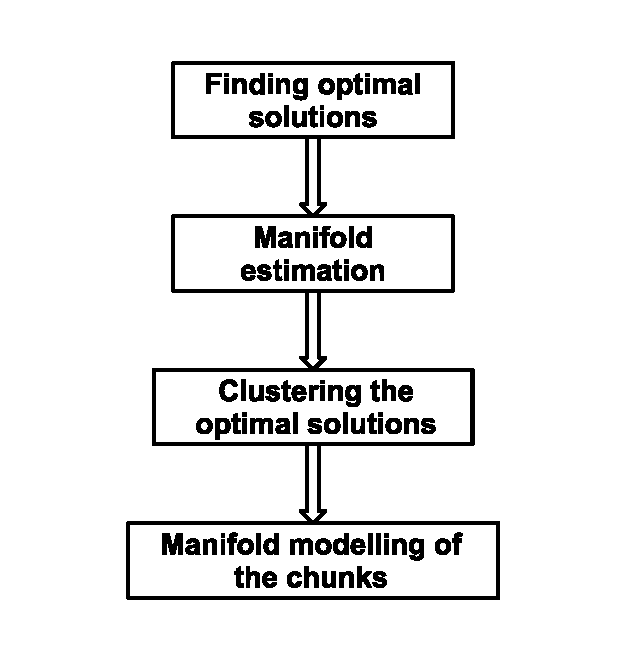
\includegraphics[width=75mm, height=75mm]{dia/overview.eps}
 \caption{Overview of the chunking process.}
 \label{overview}
\end{center}\end{figure}



\section{Obtaining set of optimal designs}
Since we want to learn chunks of ``good" solutions we must have a way of
characterising good solutions. In context of design, only the best possible
designs may be considered as good, a designer who produces feasible but
sub-optimal designs can not be called an expert. A human designer during
her routine exploration of a design problem comes across some designs that
are superior to all others. These are the designs that she is more likely
to retain in her memory as a chunk. In effect, she is searching for optimal
designs which when found are retained. The first step of our procedure to
learn patterns of good designs is to obtain a representative set of such
optimal designs.  In this section, we discuss the possible techniques of
obtaining such representative optimal solutions set.

\subsection{Conventional multi-objective optimization techniques}
In classical multi-objective optimization techniques the objectives are
combined to form one single objective using some knowledge of the problem
being solved. The optimization of the single objective-results in a single
pareto-optimal solution.

One of the classical methods of multi-objective optimization is the method
of objective weighting \citep{deb01,deb94}.  Multiple objectives are
combined into an overall objective by assigning fractional weights to the
individual objective functions which sum to one. The optimal solution is
controlled by the weight vector.

In the method of distance functions, the single objective is derived from
multiple objectives using a demand level vector $\overline{\textbf{y}}$ as
follows:\\
\begin{align}
  Z = \left[ \displaystyle\sum\limits_{i=1}^N {|f_i(\textbf{x} - \overline{y_i})|}\right] ^{1/r}, \quad &1 \leqslant r < \infty 
\end{align}\\
where $\textbf{x} \in \textbf{X}$, the feasible region. An arbitrary demand
level vector may result in a objective that doesn't have an optimal
solution, hence the decision maker must have a thorough knowledge of
individual optima of the objectives prior to the selection of the demand
level vector.

The Min-Max formulation method is different in principle from the above two
methods in that it attempts to minimize the relative deviations from the
individual optima, that is to say, it tries to minimize the objective
conflict.

The most important drawback of these classical multi-objective optimization
methods with respect to our objective is that they yield only one
pareto-optimal solution in a single run. Secondly, all of them require some
knowledge of the problem, such as the weight vector or demand
vector. Moreover it is not possible to find all pareto-optimal solutions in
some non-convex multi-objective optimization problems.

\subsection{Evolutionary algorithms for multi-objective optimization}
Evolutionary approaches to multi-objective optimization are much more
suited to the purpose of generating a representative optimal solution set,
as they can search the solution space in parallel for optimal solutions,
and produce a set of pareto-optimal solutions in a single run.

Evolutionary algorithms try to mimic the process of natural selection,
whereby only the specimens most adapted to the environment survive and
evolve. All the algorithms start with randomly chosen population of
feasible solutions and search and reproduce the best solutions in the
population. This search and reproduce procedure is repeated for many
generations, until the next generation doesn't result in significant
improvements. The first practical evolutionary multi-objective optimization
algorithm was the Vector Evaluated Genetic Algorithm (VEGA)
\citep{schaffer85}. One of the problems with VEGA is its bias towards some
pareto-optimal solutions. A non-dominated sorting procedure was proposed by
Goldberg to overcome this drawback, in which a ranking selection method is
used to emphasize good points and a niche method is used to maintain stable
sub-populations of good points.  One algorithm that that implements this
non-dominated sorting procedure is the NSGA \citep{deb94}.

This algorithm was further improved upon, and a new algorithm NSGA-II
\citep{deb02} was proposed which had better and faster convergence towards
the true pareto-front due to a fast non-dominated sorting approach. Since
it was first proposed, the NSGA-II has found application in a wide variety
of engineering optimizations and design problems. Several studies have been
published illustrating the versatility of NSGA-II in a wide variety of
situations. All these advantages that NSGA-II has over other algorithms,
and its proved versatility make it an ideal candidate for the purpose of
generating a set of pareto-optimal solutions

\subsection{The BDCPM motor design problem}
We now introduce the mulit-objective optimization formulation for the BDCPM
(brush-less DC permanent magnet motor) design problem and derive a set of
pareto-optimal solutions using NSGA-II. A BDCPM motor comprises of an outer
stator assembly with windings on a frame and inner rotor assembly having
permanently mounted magnets, shown in Figures \ref{bdcpmStator} and
\ref{bdcpmRotor}. Several variants of this basic design exist. The original
study \citep{chidam99} considered 24 slots 4 pole machine.


\subsubsection{The multi-objective optimization problem}
Figure \ref{bdcpmRotor} shows the rotor assembly of a BDCPM motor. A
ring-magnet is bonded onto a stepped shaft that fits in the bore of the
stator assembly. The total length of the motor is $L_{sh}$. The shaft
length is equal to the sum of stack length and the side clearances, $
L_{sh} = L + 2L_{cl}$. The side clearance values $L_{cl}$, and other parameters for
different lamination types are listed in Table
\ref{ltypeDimTable}.

\begin{figure}[ht]\begin{center}
 \fbox{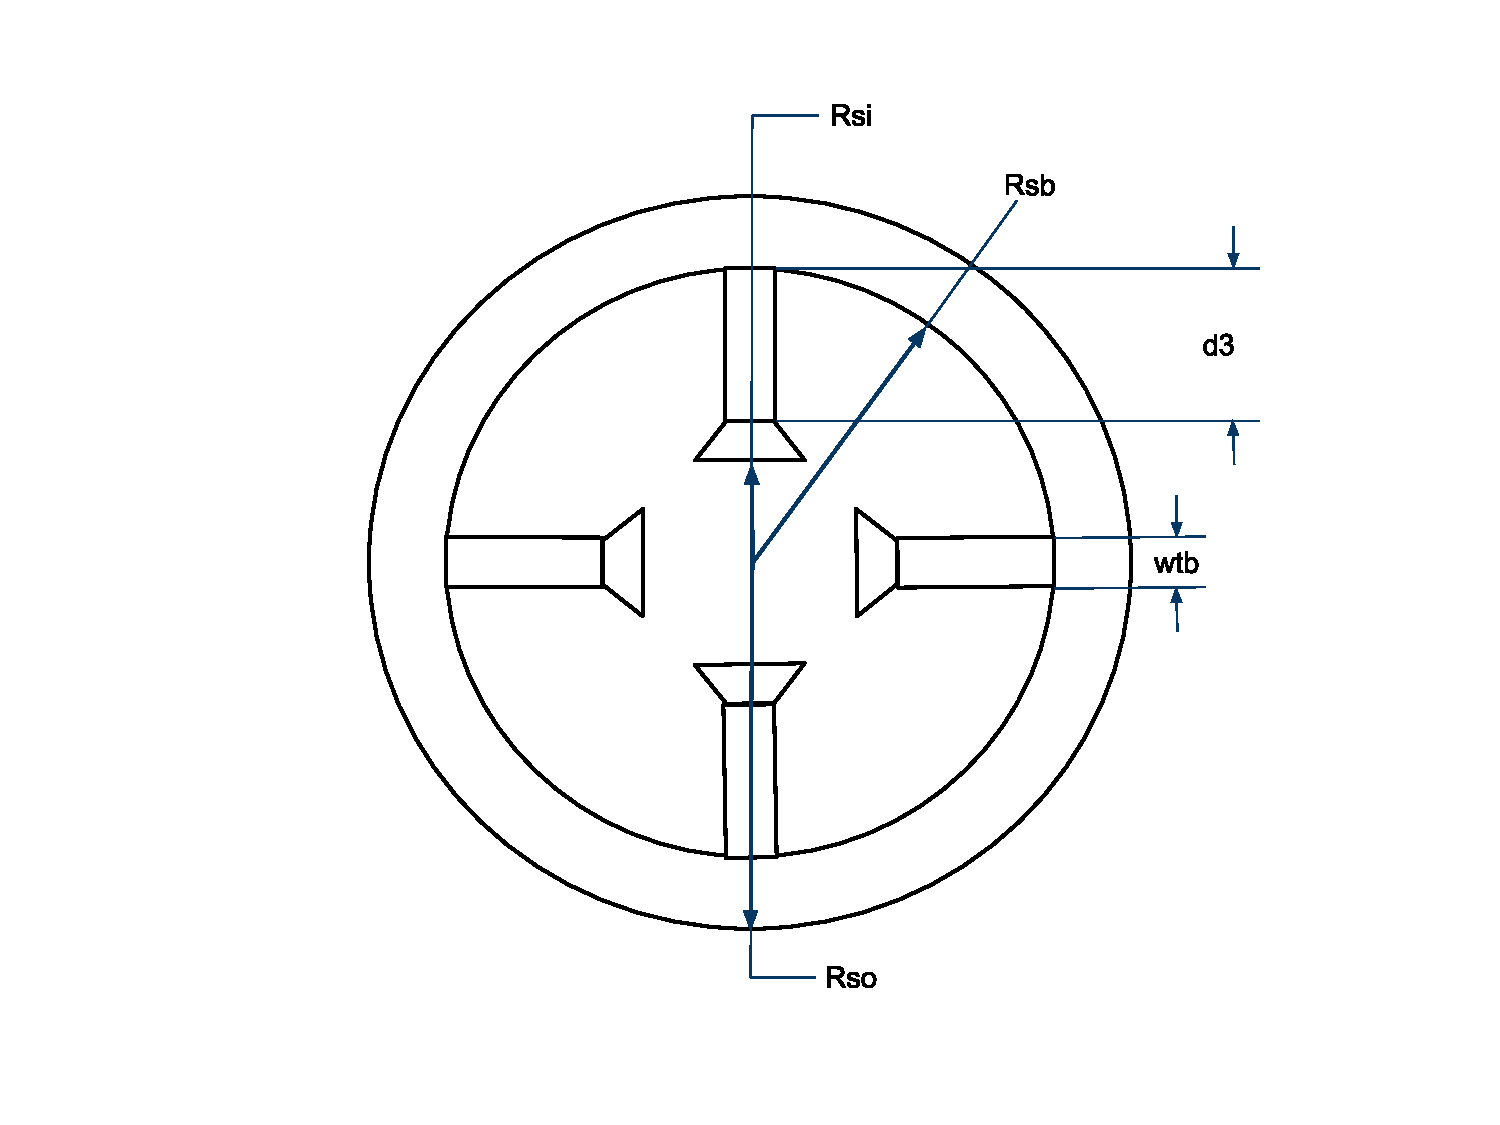
\includegraphics[width=88mm, height=65mm]{dia/bdcpmStator.eps}}
 \caption{BDCPMM Stator assembly.}
 \label{bdcpmStator}
\end{center}\end{figure}

\begin{table}[!ht]
  \centering
  \begin{tabular}{|c|c|c|c|c|c|c|c|}
    \hline
    $L_{type}$ & $R_{si}$ (mm.) & $d_3$ (mm.) & $w_{tb}$ (mm.) & $w_{bi}$ (mm.) & $L_{cl}$ (mm.)& $R_{sh}$ (mm.) & $R_{st}$ (mm) \\
    \hline
    X & 21.90 & 12.0 & 2.39 & 5.23 & 4.215 & 4.11 & 0.016 \\
    \hline
    Y & 22.22 & 15.1 & 2.39 & 5.23 & 4.265 & 4.11 & 0.016 \\
    \hline
    Z & 25.40 & 15.1 & 2.80 & 5.50 & 4.775 & 4.45 & 0.019 \\
    \hline
  \end{tabular}
  \caption{Dimensions of the BDCPM motor family}
  \label{ltypeDimTable}
\end{table}

\begin{figure}[ht]\begin{center}
 \fbox{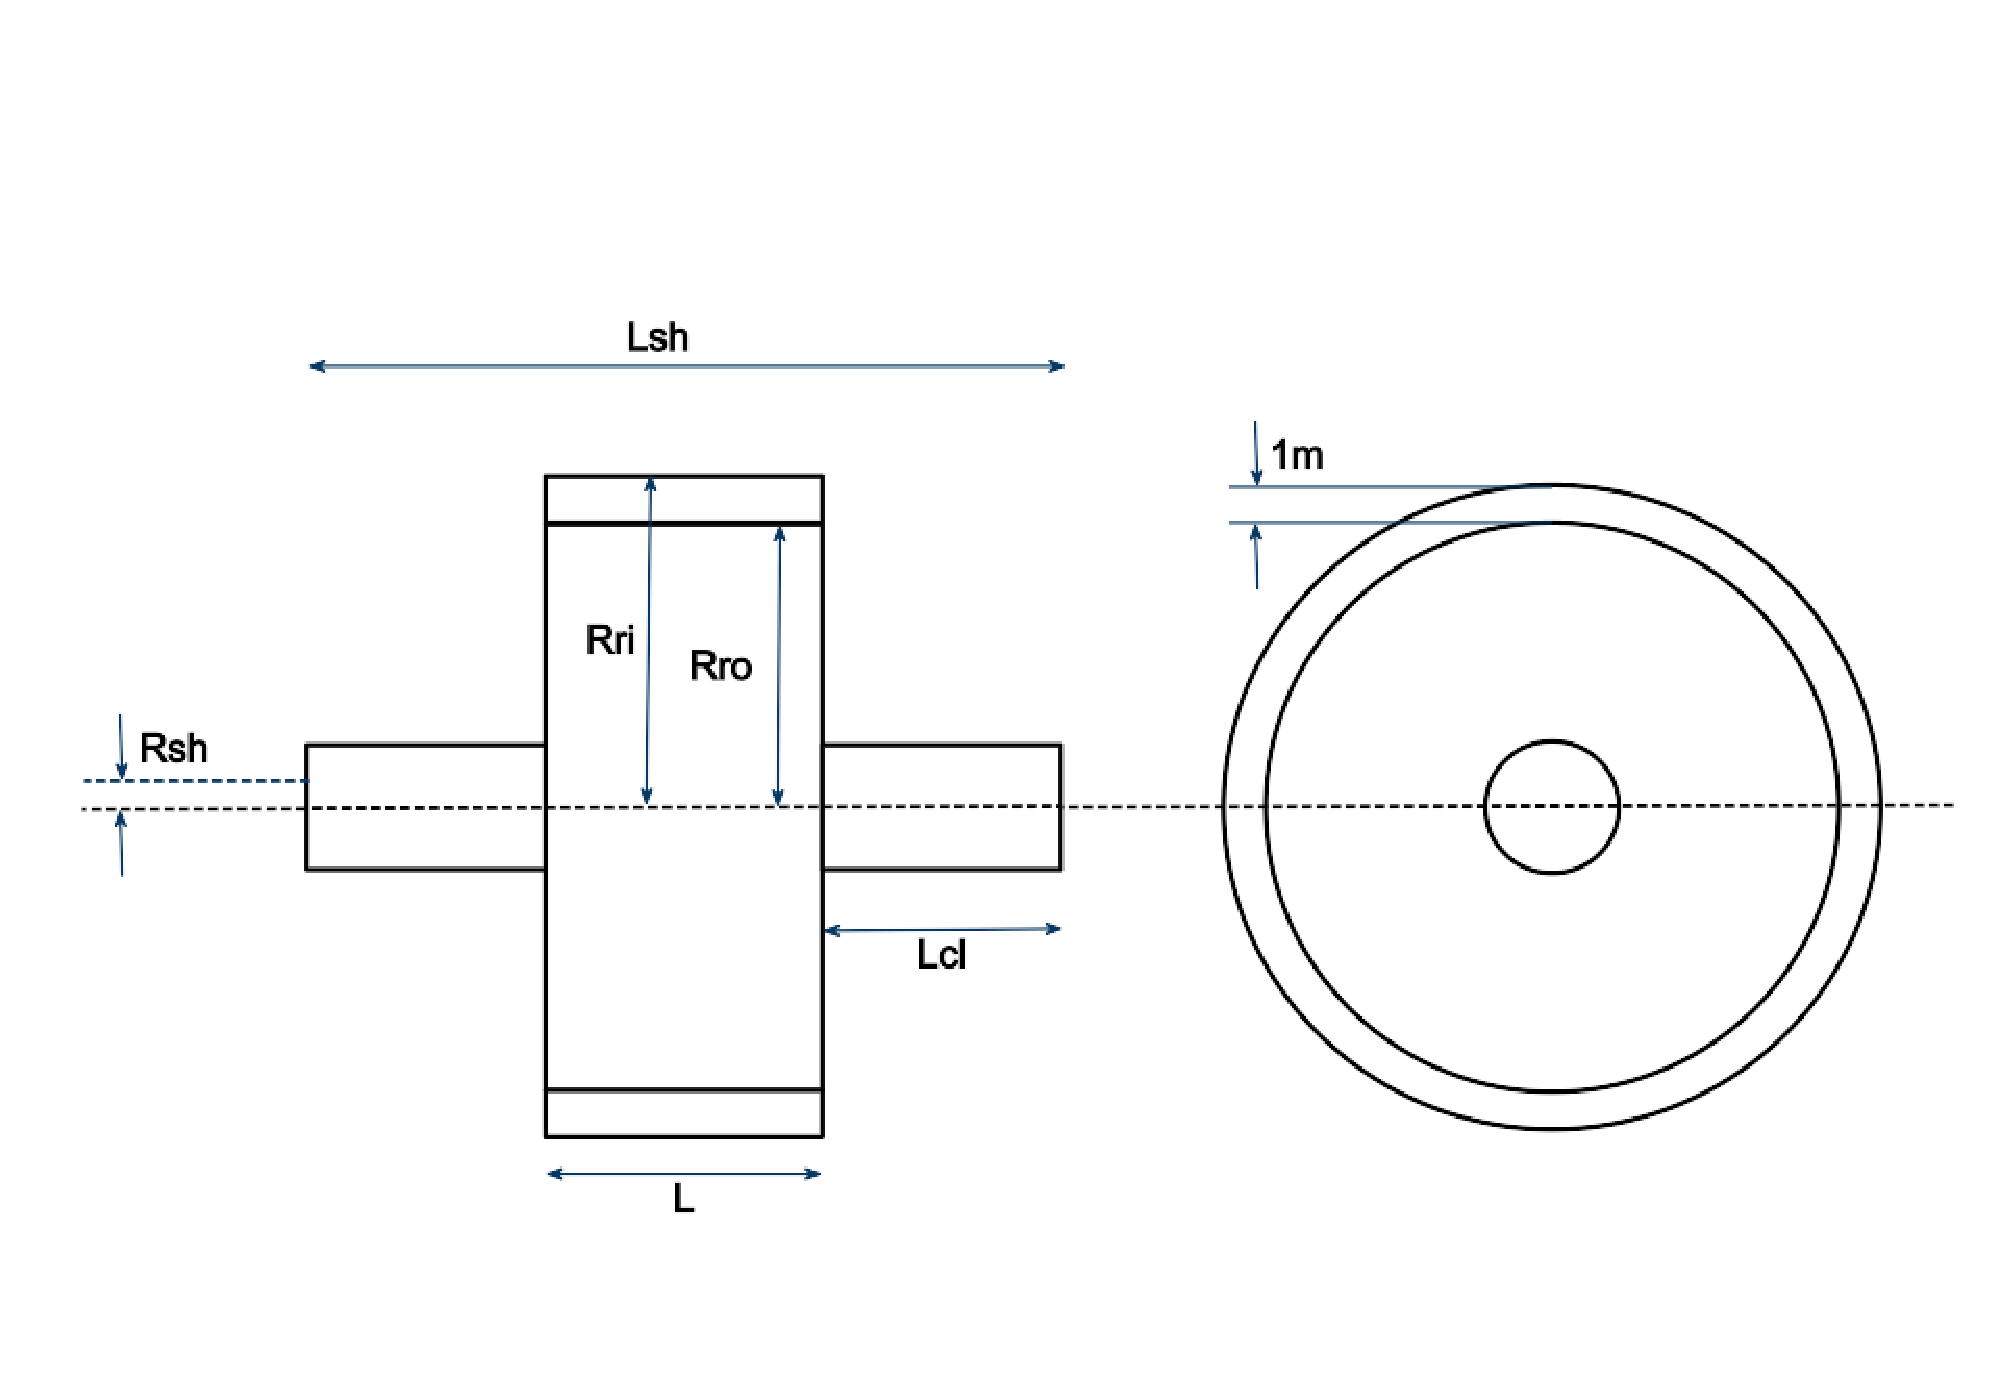
\includegraphics[width=83mm, height=59mm]{dia/bdcpmRotor.eps}}
 \caption{BDCPMM Rotor Assembly.}
 \label{bdcpmRotor}
\end{center}\end{figure}

Five design variables are considered for the design process, other design
parameters are fixed to values that are convenient for the
manufacturer. The design variables are:

\begin{enumerate}
\item Number of laminations $n_l \in [44, 45,\dots ,132]$
  
\item Number of turns in each coil  $N \in [20, 21, \dots, 80]$

\item $L_{type} \in [\textsf{X, Y, Z}]$ is one of the three types of 
laminations allowed to build the motor

\item $M_{ph} \in [Y, \Delta ]$ is one of the two types of elctric 
connections and

\item $A_{gauge} \in [16, 16.5, 17, \dots , 23.5]$ is one of the 16 
wire gauges used in the windings.
\end{enumerate}

All the design variables are discrete in nature, of which $L_{type}$ 
and $M_{ph}$ take 3 and 2 values respectively. $n_l$ and $N$ are 
integer valued variables while $A_{gauge}$ takes 16 equally spaced 
values in its domain.

The cost expression for the first objective includes the material and
estimated production cost. Each term in the expression is obtained from the
regression analyses of data obtained from practice. The detailed procedure
discribing the derivation of the cost terms and torque expressions can be
found in \citep{chidam99}.

The actual multi-objective optimization problem is formulated as follows:

%%%%%Cost function begins here%%%%%


\begin{singlespacing}

\begin{flushleft}



Minimize:   \\
$ C_{total} (n_{l}, N, L_{type}, M_{ph}, A_{wire}) = 
\begin{cases}
\quad 2.6(\frac{n_{l}}{44})^{0.25}, & \text{for $L_{type} =$ \textbf{X}} \\
\quad 0.38 + 2.42(\frac{n_{l}}{44})^{0.37}, & \text{for $L_{type} =$ \textbf{Y}} \\
\quad 1.07 + 1.83(\frac{n_{l}}{44})^{0.58}, & \text{for $L_{type} =$ \textbf{Z}} 
\end{cases} $ \\

$
+  [ \left\{0.026, 0.028, 0.03\right\}n_{l} \cong L_{type} = \{ \textbf{X}, \textbf{Y}, \textbf{Z} \} $\\
$
\, + \, \dfrac{n_{l}}{44} \, + \,   9.8 \times 10^{5} A_{wire} N [ 5.8  \times  10^{-4} n_{l}
   +  \dfrac{\pi}{2} \{ w_{tb} + \dfrac{5\pi}{12}(R_{si} + \dfrac{d_{3}}{2}) \}]
$ \\

$
+ \, 0.3035 \, + \, 0.876 N [ 5.8 \times 10^{-4} n_{l} \, + 
 \dfrac{\pi}{2} \{ w_{tb} \, + \, \dfrac{5 \pi}{12}(R_{si} \, + \, \dfrac{d_{3}}{2})\}]
$\\

$
\, + \, \pi \left[ \left\{ 31.2( R_{si} + d_{3} + w_{bi}) + 0.0312 \right\} \left\{ L_{sh} - 5.08 \times 10^{-3} \right\} \right]
$\\
$
\, + \, 
\begin{cases}
\quad 0.7(\frac{5.8 \times 10^{-4} n_{l} + 0.0792}{0.1047})^{1.21},  & \text{for $L_{type} = $ \textbf{X}} \\
\quad 0.54 + 0.26( \frac{5.8 \times 10^{-4} n_{l} + 0.0802}{0.1057})^{3.74}, & \text{ for $L_{type} =$ \textbf{Y}} \\
\quad 0.58 + 0.32( \frac{5.8 \times 10^{-4} n_{l} + 0.0905}{0.1160})^{4.23}, & \text{ for $L_{type} =$ \textbf{Z}} \\
\end{cases}
$\\
$ \, + \, 9 \, + \, \begin{cases}
\quad 1.3(\frac{5.8 \times 10^{-4} n_{l} + 0.0792}{0.1047})^{0.38} (\frac{n_{l}}{44})^{0.18}, & \text{for $L_{type} =$ \textbf{X}} \\
\quad 1.6(\frac{5.8 \times 10^{-4} n_{l} + 0.0802}{0.1057})^{0.38} (\frac{n_{l}}{44})^{0.40}, & \text{for $L_{type} =$ \textbf{Y}} \\
\quad 1.8(\frac{5.8 \times 10^{-4} n_{l} + 0.0905}{0.1160})^{0.41} (\frac{n_{l}}{44})^{0.52}, & \text{for $L_{type} =$ \textbf{Z}}
\end{cases}
$\\
$
\, + \, (1.536 R_{st} - 6.26 \times 10^{-3}) n_{l} \, + \, (2.014 R_{si} \, - \, 8.21 \times 10^{-3}) n_{l}
$\\
$
\, + \, \pi \{29.4(R_{si} - 7.25 \times 10^{-3})^{2} n_{l} \, + \, 1.014 \times 10^{5} R_{sh}^{2} L_{cl}\} 
$\\
$
\, + \, 0.1862 \, + \, 5.31 \times 10^{4} \pi [ R_{st}^{2} L_{st} \, - \,  2 R_{sh}^{2} L_{cl} 
\, - \, 5.8 \times 10^{-4} n_{l}(R_{si} - 7.25 \times 10^{-3})^{2}] 
$\\
$
 \, + \, 0.01 \, + \,0.1473 \pi (R_{si} - 7.25 \times 10^{-3}) n_{l} \, + \, \begin{cases}
\quad 1.2, & \text{for $T_{p} \le 3.5$} \\
\quad 1.6, & \text{for $T_{p} > 3.5$} 
\end{cases}
$\\
$
\, + \, \left[ \left\{ 0.5, 0.55, 0.60 \right\} \cong L_{type} = \{ \textbf{X}, \textbf{Y}, \textbf{Z} \} \right]
$\\
$
\, + \, \begin{cases}
\quad 3.2(\frac{5.8 \times 10^{-4} n_{l} + 0.0792}{0.1047})^{-1.92}(\frac{n_{l}}{44})^{0.92}, & \text{for $L_{type} = $ \textbf{X}} \\ 
\quad 3.4(\frac{5.8 \times 10^{-4} n_{l} + 0.0802}{0.1057})^{-1.92}(\frac{n_{l}}{44})^{1.06}, & \text{for $L_{type} = $ \textbf{Y}} \\ 
\quad 3.7(\frac{5.8 \times 10^{-4} n_{l} + 0.0905}{0.1160})^{-3.25}(\frac{n_{l}}{44})^{1.60}, & \text{for $L_{type} = $ \textbf{Z}} 
\end{cases}
$
\\[\baselineskip]

%%%%Torque function%%%%

Maximize: \\
$ T_p = 87300 C_{tor} N R_{si} A_{wire} n_{l} $\\
where \\
$ C_{tor} = \{ \frac{2}{3}, \frac{1}{3} \} \cong M_{ph} = \{ \textbf{Y}, \Delta  \} $ 
\\[\baselineskip]


Subject to \\
$g_1: T_{p} \geqslant 0.83$ \\

$g_2: T_{p} \leqslant 5.27$ \\

$g_3: A_{wire}N \leqslant \{150, 240, 280\} \times 10^{-7} \cong L_{type} = \{ \textbf{X}, \textbf{Y}, \textbf{Z} \}$

\end{flushleft}

\end{singlespacing}

Constraints $g_1$ and $g_2$ bound the peak torque in the desired
range. Constraint $g_3$ represents the winding constraints that prevent
magnetic saturation and demagnetization.

\subsubsection{NSGA-II formulation and the pareto-front}
Since all the variables are discrete, we use binary representation for them
in NSGA-II. We modify the population initialization routine and the EA
operators (recombination and mutation) to maintain the discrete nature of
the variables. For the two integer valued variables, $n_l$ and $N$,
discrete version of the Simulated Binary Crossover (SBX) and Polynomial
Mutation \citep{deb01} are used. Since $M_{ph}$ and $L_{type}$ take two
and three values only, they are only subjected to mutation. Using this
representation NSGA-II yields 199 non-dominated solutions, plotted in
figure \ref{nsplsp} in red circles.


\begin{figure}[ht]\begin{center}
 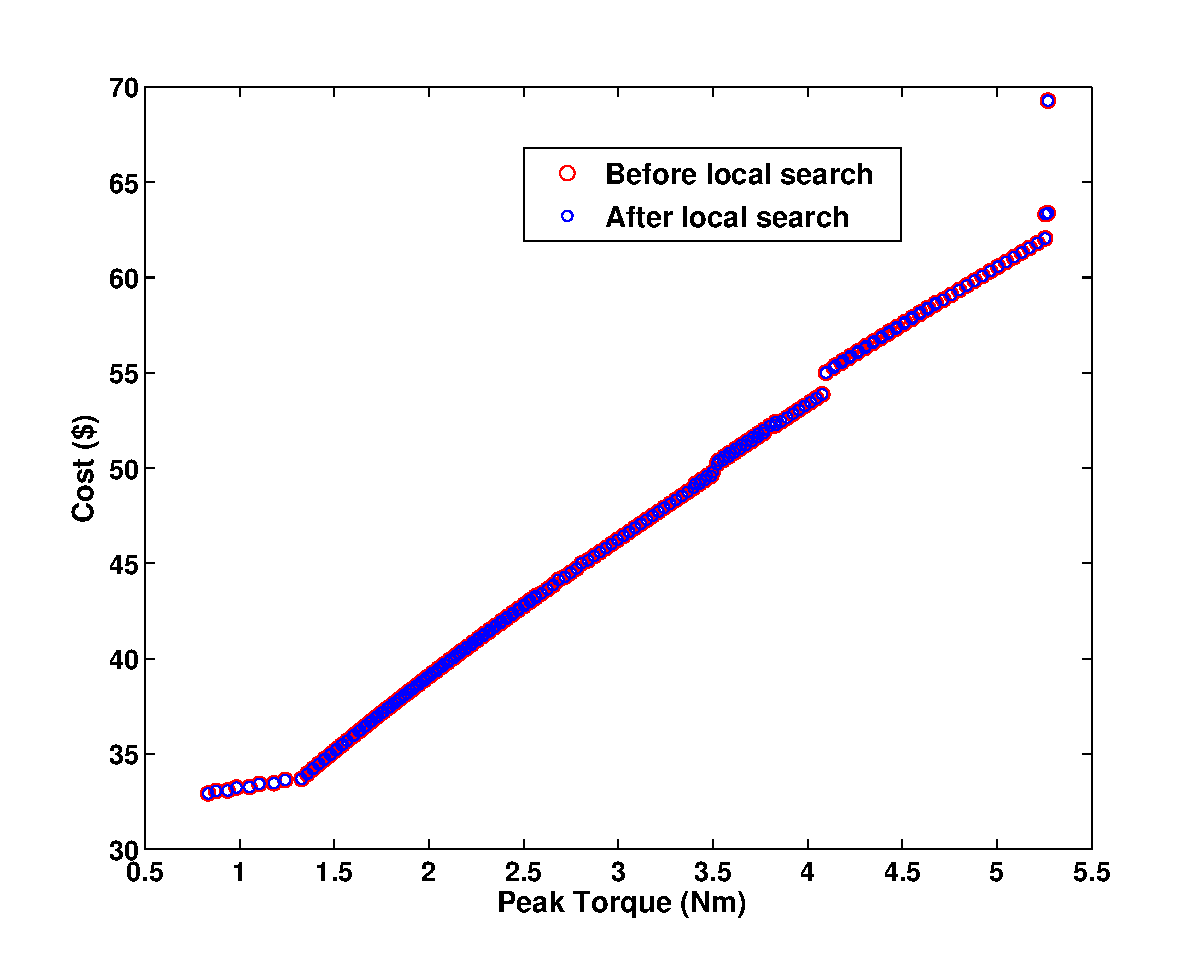
\includegraphics[width=90mm, height=75mm]{dia/nsplsp.eps} 
 \caption{Pareto-front for the BDCPMM design problem. The red circles represent the design results of NSGA-II and the blue circles represent the design results of the local search. Pareto-front obtained after the local search overlaps with the NSGA-II result.}
 \label{nsplsp}
\end{center}\end{figure}


\subsection{Local search procedure}
Although an evolutionary procedure may find a set of near optimal solutions
quickly, the convergence to the true pareto-front might take indefinitely
long. To improve convergence characteristics of the evolutionary
multi-objective algorithms they are often complemented with a local search
procedure. Local search is more important in case of multi-objective
optimization problems which involve discrete variables.  We have used a
generic local search procedure which evaluates random solutions in the
vicinity of the near-optimal solution under consideration. The input for
local search are the set of near optimal solutions $S$, number of local
search iterations to perform $n$, number of local solutions to evaluate for
each near optimal solution $h$, and the search width factor
$\sigma$. Algorithm \ref{localsearch} gives the pseudo-code for our local
search procedure.

\begin{algorithm}
  \SetKwInOut{Input}{input}\SetKwInOut{Output}{output}
  \Input{($S$, $n$, $h$, $\sigma$)}
  \Output{Set of optimal solutions $P$}
  $P = \phi$;\\
  \For{$i = 0$ to $n$}{
    \For{each $s \in S$}{
      add $s$ to $P$;\\
      find $k$ nearest neighbors of $s$;\\
      find the range of values each variable takes in the $k$-neighborhood;\\
      \For{$j = 0$ to $h$ }{
        generate a candidate random solution $p$ having variable values in the 
        neighborhood range scaled by $\sigma$;\\
        add $p$ to $P$;
      }
    }
    perform non-dominated sorting on $P$ and discard dominated solutions;\\
    $S$ = $P$;
  }
  return $P$;
  \BlankLine
  \caption{Local search procedure.}
  \label{localsearch}
\end{algorithm}

For the BDCPMM design problem, however, local search doesn't result in much
improvement since we ran NSGA-II for a large number of generations(3000)
which would have been sufficient for convergence to the actual
pareto-front. Performing local search on the NSGA-II output for BDCPMM
design problem increases the number of optimal solutions to 201 from 199.

\section{Estimating the pareto-front manifold}
We apply Isomap and PCA to estimate the dimensionality of the pareto-front
manifold and learn global properties of the set of the good designs. After
clustering this process will again be applied to the obtained chunks to
elicit the chunk local properties and capture their semantics.

% If $k$ conflicting objectives have to be optimised simultaneously in a
% multi-objective optimization, the resulting pareto-front would be a $k-1$
% dimensional manifold in the obejctive space. Modelling the pareto-front as
% a manifold may reveal how the objectives are related to each other, whether
% they are mutually conflicting in which case we will get a $k-1$ dimensional
% manifold, or some of them vary directly with each other, then the manifold
% will be of dimension less than $k-1$.  Similarly a linear dimensionality
% reduction analasys using PCA may reveal the relative importance of the
% decision variables in the optimal solutions.
  
\subsection{Isomap Residual Variance for the Pareto-front}
On performing Isomap on the pareto-front data of BDCPMM design we obtain a
residual variance plot shown in figure \ref{isoRVbdcpmAll}.  Since the
residual variance shows a sharp decline going from one dimensional
embedding to two-dimensional embedding, we can expect the pareto-front to
be composed of sub-manifolds of one or two dimensions.  There is an
unexpected increase in the residual variance for three dimensional
embedding, though it drops down to the previous level for four dimensional
embedding.

\subsection{PCA explained variance}
The PCA analysis of BDCPMM pareto-front gives four principal
components. The explained variance for principal components of the BDCPMM
pareto-front data are plotted in figure \ref{pcaEVbdcpmAll}.  The first
principal component has explained variance of more than 0.95, while the
second principal component has explained variance of 0.021.  The third and
fourth principal components have negligible explained variances. Table
\ref{first2BDPCs} shows the first two principal component vectors which
reveal that the pareto front is a manifold embedded in the plane of first
two design dimensions, namely number of laminations and number of turns in
the stator windings.
 

\begin{figure}[ht]\begin{center}
    \subfloat[Isomap Residual Variance.]{
      \label{isoRVbdcpmAll} 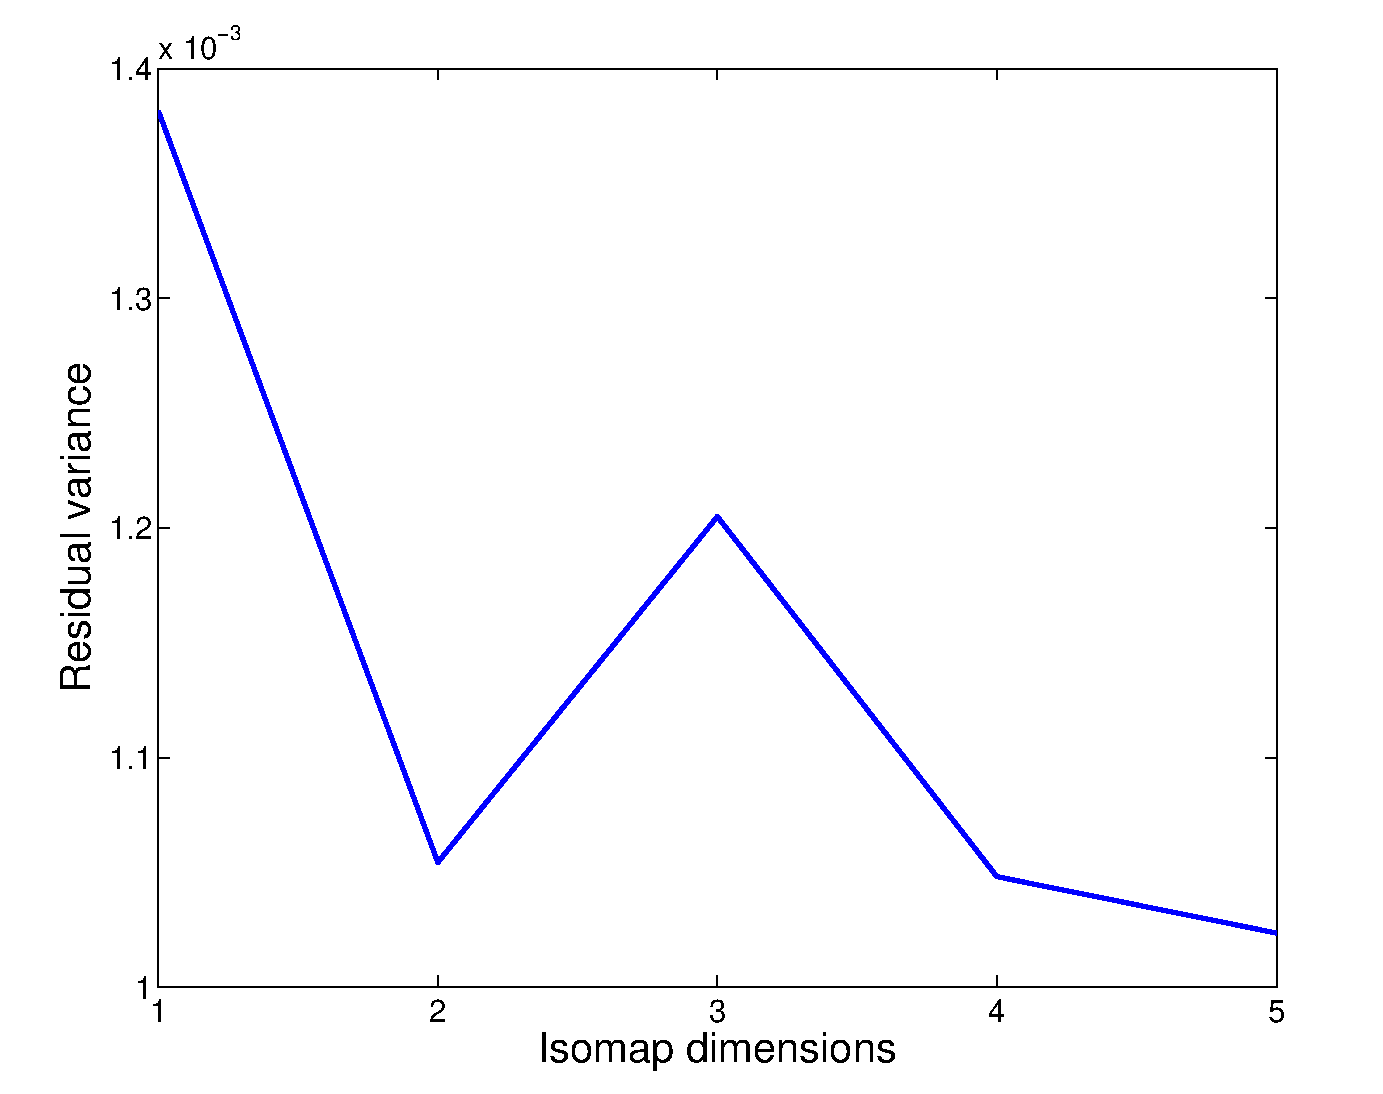
\includegraphics[width=62mm, height=52mm]{dia/isoRVbdcpmAll.eps}}
    \subfloat[PCA Explained variance.]{
      \label{pcaEVbdcpmAll} 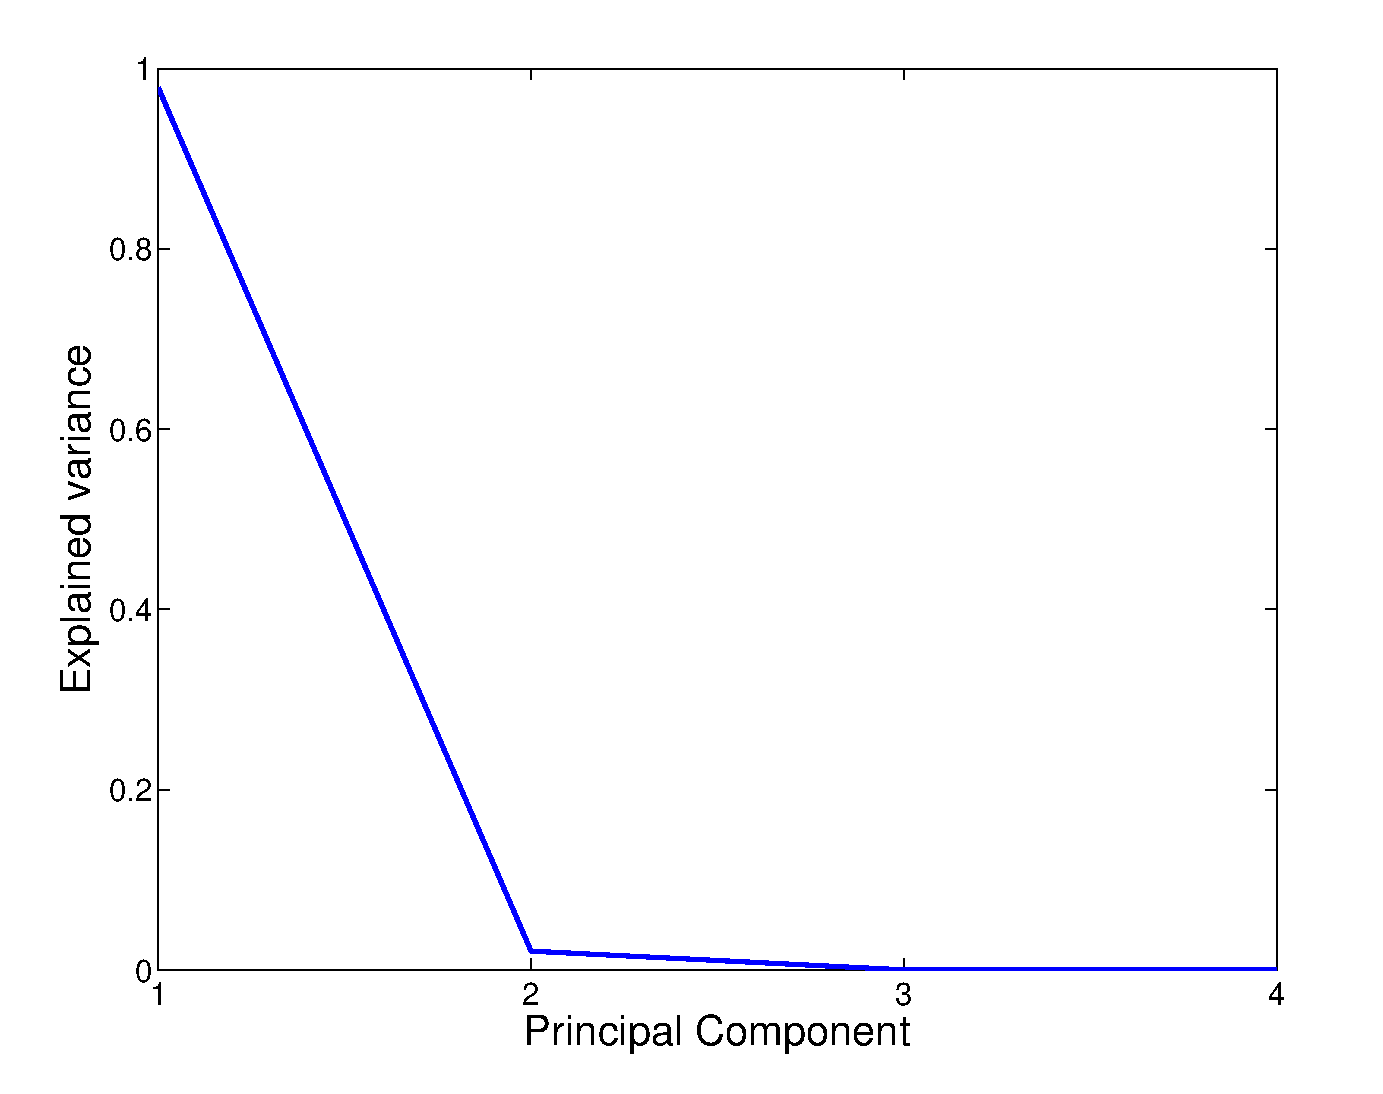
\includegraphics[width=62mm, height=52mm]{dia/pcaEVbdcpmAll.eps}}
    \caption{Isomap and PCA results. The residual variance plot shows the
      largest drop for the second dimension indicating a manifold of
      dimension one. First principal component has an 95\% explained
      variance indicating a linear dimensionality of one.}
    \label{bdcpmmVar}
  \end{center}
\end{figure}

\begin{table}[!ht]
  \centering
  \begin{tabular}{c|c|c|c|c|c|}
    \cline{2-6}
    & $n_l$ & $N$ & $ L_{type} $  & $ M_{ph}$ & $a_{gauge}$ \\
    \hline
    \multicolumn{1}{|c|}{First PC} & 0.9993 & 0.0370 & 0.0072 & 0 & -0.0024\\
    \hline
    \multicolumn{1}{|c|}{Second PC} & -0.0367 & 0.9943 & 0.0165 & 0 & 0.0985\\
    \hline
  \end{tabular}
  \caption{First two principal components of the BDCPM data. Number of laminations is the dominant variable in the first principal component.}
  \label{first2BDPCs}
\end{table}


\section{Clustering the pareto-front}
Our chunking process aims to identify solutions with similar
characteristics and group them together. Those solutions of a
multi-objective optimization which are close together in the combined
objective-decision variables space, can be expected to have some shared
characteristics. Clustering the pareto-front is a way to group similar
solutions together.

\begin{figure}[ht]
  \begin{center}
    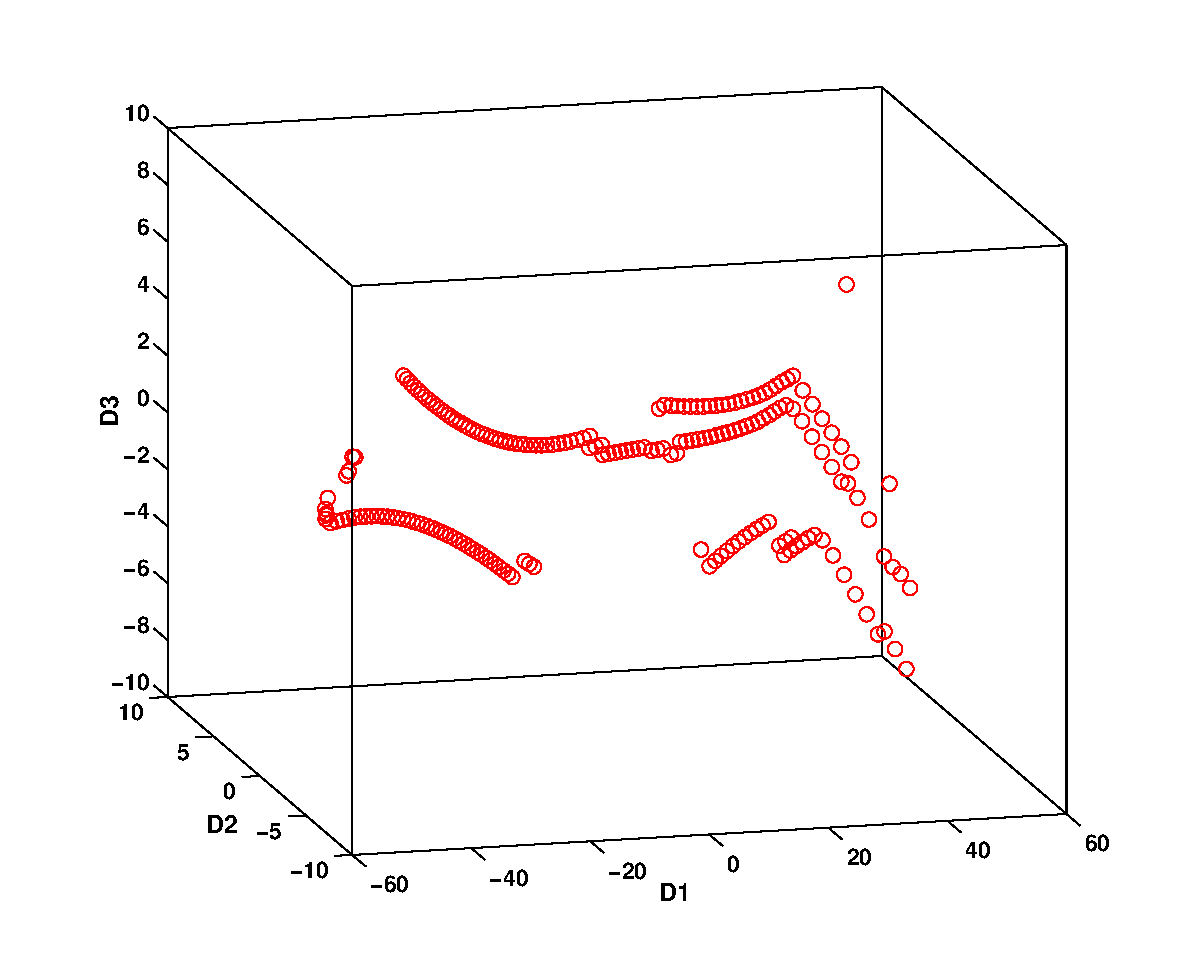
\includegraphics[width=90mm, height=75mm]{dia/bdcpmiso3.eps} 
    \caption{3-dimensional Isomap Embedding of the BDCPMM problem
      pareto-front, showing several one-dimensional manifolds.}
    \label{bdcpmiso3}
  \end{center}
\end{figure}

Figure \ref{bdcpmiso3} shows the 3-dimensional Isomap embedding of the
BDCPMM pareto-front. The embedding algorithm used in the Isomap is the
classical multi-dimensional scaling (cMDS), which aims to preserve the
inter-point distances in the reduced dimension. The 3-dimensional Isomap
embedding is thus an approximate modelling of the data set in the original
parameter space, with distances along the manifold preserved. This figure
clearly suggests that the BDCPMM pareto-front is composed of
one-dimensional manifolds, some of which run parallel to each other. Our
aim in clustering the pareto-front is to recover these lower dimensional
sub-manifolds.

We use an algorithm that is based on concepts of density-based partitioning
to cluster the pareto-fronts. One advantage of density based clustering is
that it is able to discover clusters of arbitrary shapes. DBSCAN is a major
representative of density based clustering.  DBSCAN works by identifying
\emph{core objects} in the data, those points in the data-set that have
at least $MinPts$ points within their $\epsilon$-neighborhoods. Two points
$x$ and $y$ have \emph{density connectivity} between them if there exists a
sequence of core objects between $x$ and $y$ such that each next belongs to
an $\epsilon$-neighborhood of its predecessor. Two points with density
connectivity between them belong to the same cluster. $MinPts$ and
$\epsilon$ are the only two parameters that this algorithm requires.

Our variant utilizes the concept of density connectivity, but we do not
attempt to explicitly identify the core objects. Instead, density
connectivity between points is determined by building a graph based on
density. Initially, all the points in the data-set are nodes in the
graph. We start by finding $n_{max}$ nearest neighbors of each point in the
data-set and sort these lists of nearest neighbors in the increasing order
of their distances from the point. At the beginning of each iteration, the
average edge weight ($ad_c$) and edge weight standard deviation
(${\sigma}_c$) are calculated for each component.  We connect each point
$p$ with the first point in its nearest neighbor list only if its distance
from the point is within $k{\sigma}_c + ad_c$ for the component $c$ to
which $p$ belongs, or else if average edge weight in the component is zero
($p$ is not connected to any other node), then average global inter-point
distance is used in place of $ad_c$. If an edge is added then the nearest
neighbor is popped from the list, otherwise we don't process $p$ in
subsequent iterations, as it means that either $p$ is an outlier or a
boundary point of the cluster. This process is repeated for $n_{max}$
iteration, by which time all the nearest neighbors lists will be empty. The
pseudo-code of the algorithm is shown in the listing \ref{clusteralgo}.

Our variant differs from DBSCAN in two important aspects. First, our
algorithm allows for clusters with different intra-cluster point densities,
since the decision that a point belongs to a cluster is based on its
distance from the nearest point in the cluster, and the average edge weight
within the component.  DBSCAN may fail to identify a cluster with lower
point density because of a low $\epsilon$ parameter. Secondly in place of
the $\epsilon$ parameter we have $n_{max}$ parameter giving the number of
nearest neighbors that must be found for each point. The number and size of
clusters depends on the parameter $k$.


\begin{algorithm}
  \SetKwInOut{Input}{input}\SetKwInOut{Output}{output}
  \Input{($D$, $n_{max}$, $k$)}
  \Output{A cluster labelling for each data-point}
  \BlankLine
  find $n_{max}$ nearest neighbors of each point arranged in non-decreasing
  order of the distance;\\
  $ad_{g} =$ average inter-point distance in the data set;\\
  ${\sigma}_g =$ standard deviation of distances in the data set;\\
  $G =\{V, E\}$ be a graph where $V$ is the set of all data-points and $E = \phi$;\\ 
  \For{$i = 1$ to $n_{max}$}{
    \For{each connected component $c$ in $G$}
    {
      find out the average and standard deviation of edge weights in $c$;\\
    }
    \For{each point $p$ in the data set}
    {
      \If{ $p$'s nearest neighbor list is empty}
      {
        continue;\\
      }
      $c =$ component label of the component $p$ belongs to; \\
      $q =$ the first point in the nearest neighbor list of $p$;\\
      $d =$ distance to first point in ordered nearest neighbors list of $p$;\\
      \eIf{i = 0}
      {
        $thresholdDistance = ad_g + k {\sigma}_g$ ;\\
      }
      {
        $thresholdDistance = ad_c + k {\sigma}_c$ ;\\
        \tcc{$ad_c$ and ${\sigma}_c$ are the average and standard deviations of edge weights in $c$}
      }
      
      \eIf{$d > thresholdDistance$}
      {
        \tcc{if $i = 0$ then $p$ is either an outlier or boundary}
        remove all points from the ordered nearest neighbors list of $p$;\\
      }
      {
        \If{ $(q, p) \notin E$}
        {
          add ($p$, $q$) to $G$;\\
          remove $q$ from ordered nearest neighbors list of $p$;\\
        }
      }
    }
  }
  label points in $V$ with the component they belong to; \\
  return $V$;\\
  
  \caption{Clustering algorithm to obtain low-dimensional clusters}
  \label{clusteralgo}
\end{algorithm}


The clustering of the BDCPMM pareto-front results in five clusters which
are shown in the objective space plot in figure \ref{bClustersO}.  Figure
\ref{bClustersP} shows the clusters with respect to the number of
laminations ($n_l$) and the number of turns ($N$) in the stator windings.
Other design variables are indicated alongside the clusters.

\begin{figure}[ht]
  \begin{center}
    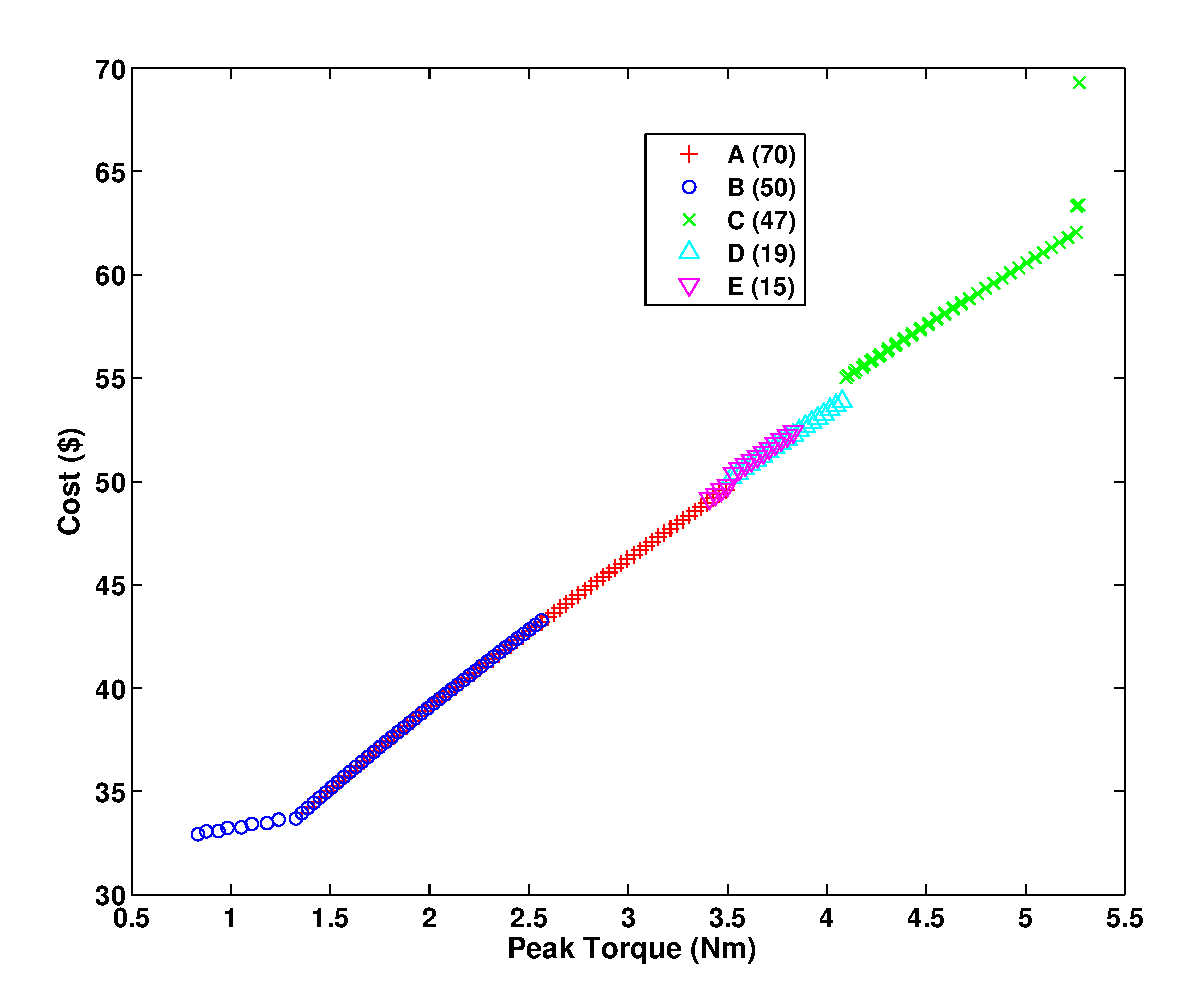
\includegraphics[width=100mm, height=80mm]{dia/bClustersO3.eps} 
    \caption{Clusters in the BDCPMM pareto-front. Clusters \textbf{A} and
      \textbf{B} are composed of low power and cost designs while Cluster
      \textbf{D} as the high-power and cost designs.}
    \label{bClustersO}
  \end{center}
\end{figure}

\begin{figure}[ht]
  \begin{center}
    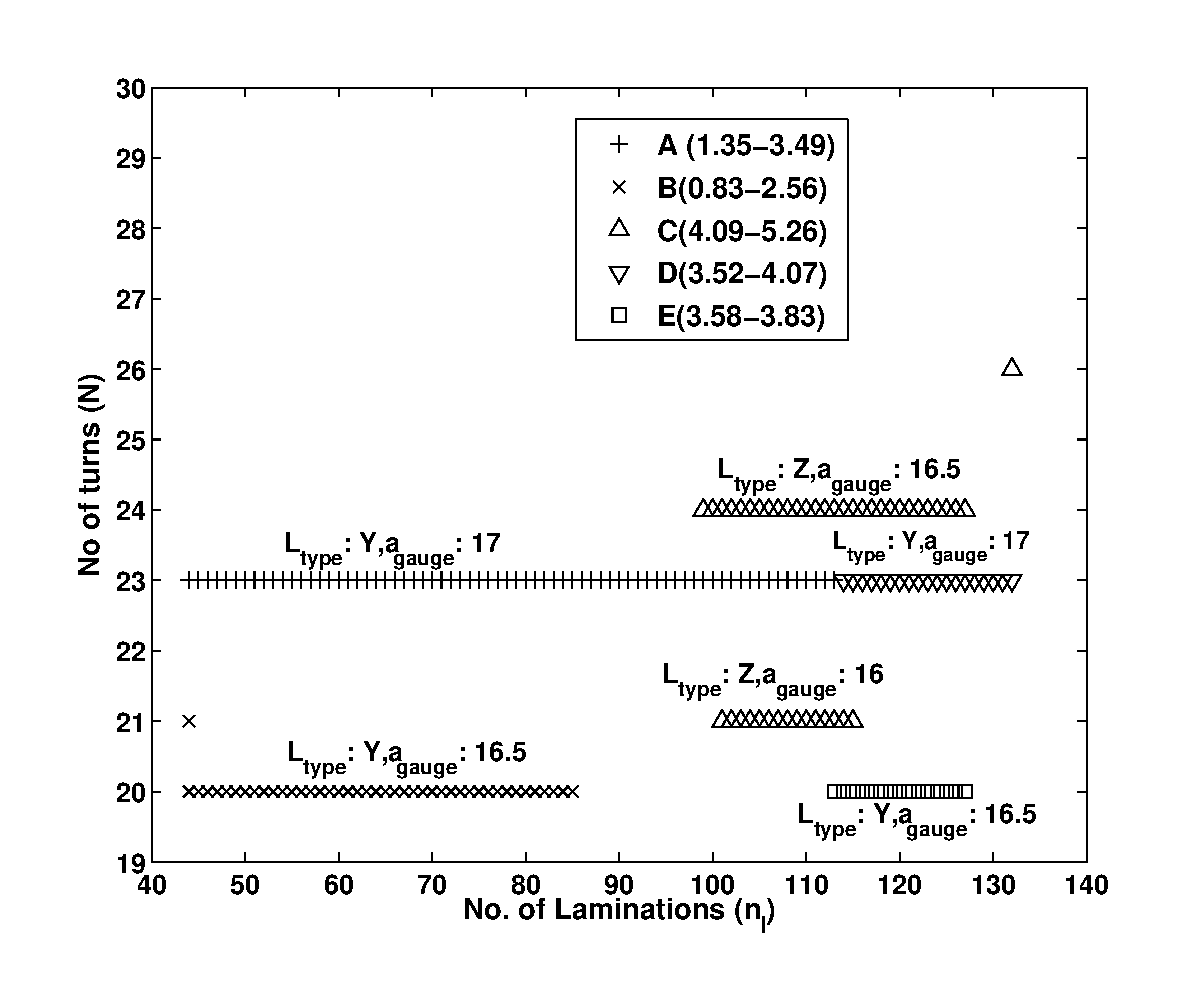
\includegraphics[width=100mm, height=80mm]{dia/bclustersp3.eps} 
    \caption{Clusters in the $n_l$-$N$ subspace. All the clusters appear as
      lines in the parameter space except the cluster of high-end designs
      \textbf{D} which appears as two separate lines.}
    \label{bClustersP}
  \end{center}
\end{figure}
 
\section{Manifold modelling of the clusters}
In this step we apply manifold learning and linear dimensionality reduction
to the clusters obtained in the previous step in an attempt to uncover the
nature of the clusters. We again use Isomap to uncover the shape and
dimensionality of each cluster and PCA to elicit shared design
characteristics of solutions in each cluster. However, since the clusters
may be linear patches of the whole manifold, PCA analysis reveals more
useful information than Isomap analysis. All the clusters except \textbf{C}
have negligible or zero residual variance for one dimensional Isomap
embedding, indicating that they are one-dimensional.  Residual variances
for \textbf{C} are plotted in figure \ref{bClusterCrv}. The residual
variance shows a large drop from two dimensional Isomap embedding to three
dimensional Isomap embedding, after which it is flat. This means that
cluster \textbf{C} has intrinsic dimensionality of two. Looking at figure
\ref{bClustersO} and \ref{bClustersO} reveals why it is so. The cluster
\textbf{C} has higher torque motors, but unlike other clusters which have
the same number of turns in the stator windings, it has two types of
designs with 21 and 24 turns. The wire gauges are also distinct in these
two types of designs, those with 21 turns use 16 gauge wire and those with
24 turns use 16.5 gauge wire.

These findings are in accordance with the {\em chunk dimensionality
  conjecture} proposed in section \ref{cdc}, whereby chunks are manifolds
in the decision space of dimensionality less than the dimensionality of the
decision space. The dimensionality of these manifolds in the decision space
is also less than or equal to the dimensionality of the objective space,
which is two in this case. Four clusters have manifold dimensionality of
less than two and only one has two dimensions.

 
\begin{figure}[ht]
  \begin{center}
    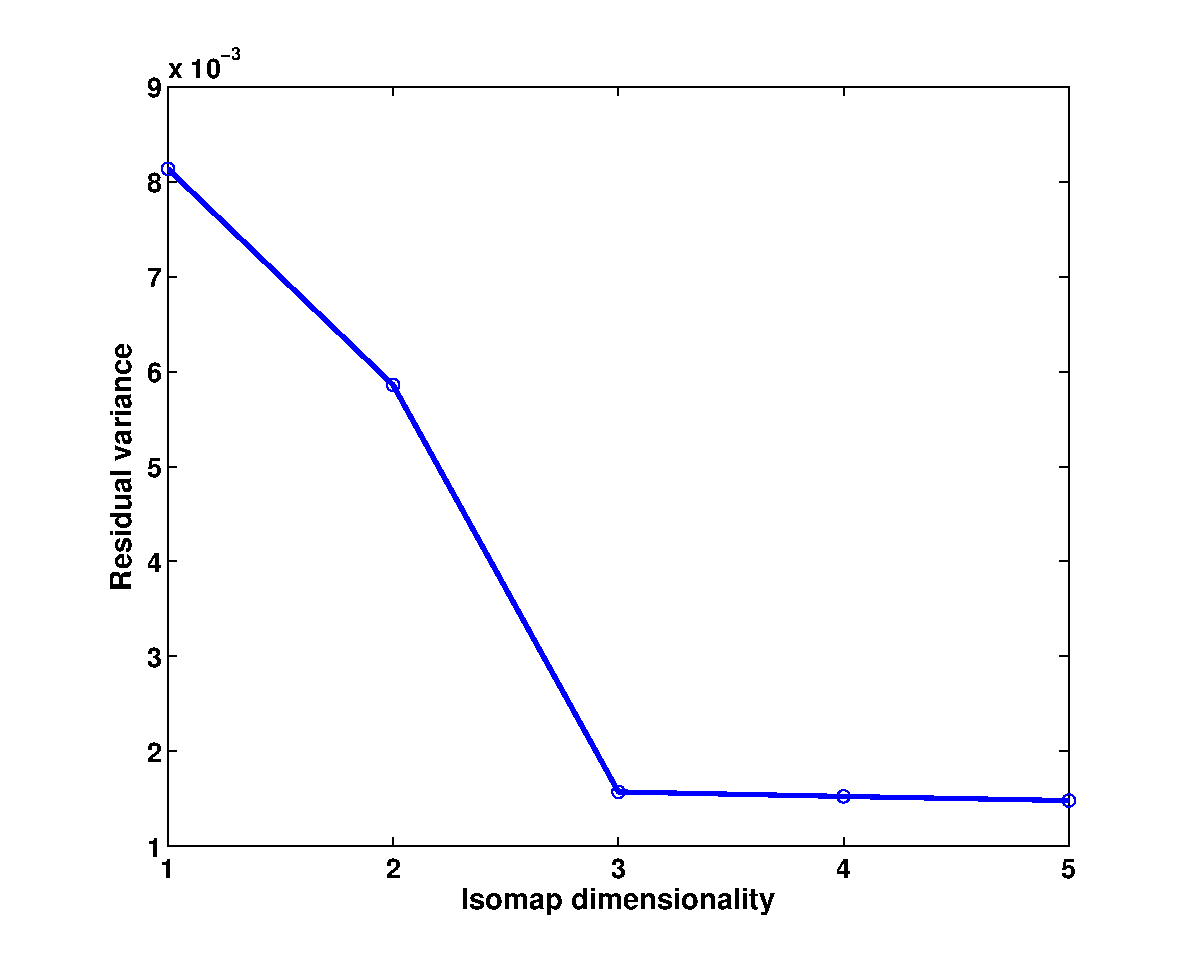
\includegraphics[width=60mm, height=50mm]{dia/bclusterCrv.eps} 
    \caption{Residual variance for the cluster \textbf{C}. The largest drop
      in the residual variance is for the 3-dimensional Isomap embedding,
      indicating a two dimensional manifold.}
    \label{bClusterCrv}
  \end{center}
\end{figure}

Table \ref{clustersEV} shows the explained variances for principal
components of each of the clusters. The explained variances corroborate the
observations made in the Isomap analysis that four of the clusters are one
dimensional and only one cluster (\textbf{C}) is two dimensional. Table
\ref{clusterPC} lists the first principal components of the clusters
\textbf{A}, \textbf{B}, \textbf{D} \textbf{E}. Since cluster \textbf{C} is
two dimensional, its two principal components are shown.

\begin{table}[!ht]
  \centering
  \begin{tabular}{|c|c|c|c|c|c|}
    \hline
    \textbf{A} & 100 & 0 & 0 & 0 & 0 \\
    \hline
    \textbf{B} & 99.857 & 0.119 & 0.02 & 0 & 0\\
    \hline
    \textbf{C} & 70.82 & 29.17 & 0.01 & 0 & 0\\
    \hline
    \textbf{D} & 100 & 0 & 0 & 0 & 0\\
    \hline
    \textbf{E} & 100 & 0 & 0 & 0 & 0\\
    \hline
  \end{tabular}
  \caption{Explained variances for the principal components of the clusters. For clusters \textbf{A}, \textbf{B}, \textbf{D} and \textbf{E} there is only one significant principal component. Cluster \textbf{D} has two significant principal components.}
  \label{clustersEV}
\end{table}

\begin{table}[!ht]
  \centering
  \begin{tabular}{c|c|c|c|c|c|}
    
    \cline{2-6}
    & $n_l$ & $N$ & $ L_{type} $  & $ M_{ph}$ & $a_{gauge}$ \\
    \hline
    \multicolumn{1}{|c|}{\textbf{A}} & 1 & 0 & 0 & 0 & 0 \\
    \hline
    \multicolumn{1}{|c|}{\textbf{B}} & 0.999 & 0.0077 & 0 & 0 & -0.019\\
    \hline
    \multicolumn{1}{|c|}{\multirow{2}{*}{\textbf{C}}} & 0.789 & 0.610 & 0 & 0 & 0.066\\ \cline{2-6}
    \multicolumn{1}{|c|}{}& -0.613 & 0.785 & 0 & 0 & 0.074\\
    \hline
    \multicolumn{1}{|c|}{\textbf{D}} & 1 & 0 & 0 & 0 & 0\\
    \hline
    \multicolumn{1}{|c|}{\textbf{E}} & 1 & 0 & 0 & 0 & 0\\
    \hline
  \end{tabular}
  \caption{Principal components for the clusters. For \textbf{A} \textbf{B} \textbf{D} and \textbf{E} the principal component is along the direction of $n_l$. Cluster \textbf{C} has two components which are in the $n_l - N$ plane. }
  \label{clusterPC}
\end{table}

\section{Design implications}
There are a number of important facts that can be observed from the PCA
analysis of the clusters. Firstly, as is evident in the tables
\ref{first2BDPCs} and \ref{clusterPC}, number of laminations is the most
important design parameter, as this is the variable that has the largest
weights in the first principal component of the whole pareto-front and the
clusters. This parameter can be changed for inducing a small amount of
change in the peak torque and cost.

The connection type ($M_{ph}$) has no contribution whatsoever in the
principal components of the pareto-front and the clusters. This means that
all the optimal designs must be using the same connection type. Only
\emph{Y} connection type is used in all the designs.
 
Although the variable $L_{type}$ has no weight in the principal
components of the clusters, it has some contribution to the principal
component of the overall pareto-front. This means that lamination type is
the same for all the designs in a single cluster, though it may vary across
the pareto-front. Only two out of three lamination types are used in all
the designs. Lamination type Y is used in all the clusters except
\textbf{C}, in which lamination type Z is used.  Looking at figure
\ref{bClustersP} we can see that cluster \textbf{C} occupies the highest
torque and cost range of the pareto-front. This implies that lamination
type Z is only useful for high end designs of BDCPM motors.

Number of turns ($N$) has a small weights in the principal components of
the pareto-front. The principal components of clusters \textbf{A},
\textbf{D} and \textbf{E} have zero weights for $N$, and \textbf{B} and
\textbf{C} have non-zero weights. Incidentally, these are also the only
clusters that have non-zero weights for the variable $a_{gauge}$. This
suggests that these two variables are not independent of each other in the
optimal designs. The number of turns tend to stick to the lower region
(20--24) of the range of possible values (20--80). Also higher
cross-section wires (lower $a_{gauge}$) among the available choices are
used in the optimal designs

\section{How the chunks relate to experts' intuition}
\label{bdcpmDiscuss}
The observations made in the previous section are in confirmation of the
expert's intuition of the design of a BDCPM motor, discussed in the section
\ref{expertInAction}. To the expert it was `natural' that if higher peak
torque is desired then number of laminations have to be increased
proportionately. Increasing the number of turns in the stator winding also
increases the torque, but in much larger quanta's. Also, since
non-customizable lamination designs are used, it may not be possible to
increase the number of turns, the reason being that the size of the groove
($d_3$ in figure \ref{bdcpmStator} and table \ref{ltypeDimTable}) that
accommodates the windings is fixed for each lamination type. So to increase
the number of turns either a lamination type with larger radial dimensions
must be used or a wire with smaller cross-section must be chosen for the
windings.

All these trade-offs can be clearly observed in play in the cluster of
high-end designs (\textbf{C}) where the lamination type with largest radial
dimension is used and two combinations of number of turns and wire
cross-section are employed. One set of designs has 21 turns with 16 gauge
wire and the other has 24 turns with 16.5 gauge wire.


When the expert had to choose the connection type in the winding, he chose
the {\em Y} type connection, although reasons for the choice were not
immediately clear. After some back of the envelop calculations, the
explanation he gave was that since the wire cross-section is fixed, the
maximum current that can flow in the stator winding is limited and {\em Y}
connection type allows for a higher power factor. Indeed, all the optimal
designs in our results have a {\em Y} connection type.

 
\chapter{The Gearbox Design Problem}
The Gear Train design problem is a classic multi-objective optimization
problem, for it encompasses a number of the challenges that a practical
real world optimization task may present. It involves a number of variables
of different types and a large number of equality and inequality
constraints. A number of objectives can be considered for the
optimization. This problem was analyzed in \citep{agogino90} to explain the
design process from an optimization perspective, and in \citep{debgt} to
prove the applicability of NSGA-II in complex optimization tasks. We
analyze the pareto-optimal solutions of this design-optimization problem to
discover chunks of optimal designs using our proposed procedure.


\section{Problem description}
\label{problem}
The objective of multi-speed gearbox design is to obtain different
specified speeds in the output shaft with fixed input shaft angular
velocity. The two-dimensional layout of a 18-speed gearbox with 18 gears is
shown in figure \ref{geartrain}. Gears in shafts 1, 3 and 5 can be
translated to mesh with corresponding gears in shafts 2, 4 and 6 to obtain
desired output speed. The input shaft speed is kept fixed at 1400 rpm. With
a ratio of 1.14 between consecutive output speeds, the $i^{th}$ desired
output speed would be $1400/(1.14)^{i-1}$.  The lowest desired speed is
thus $1400/(1.14)^{17} = 150$ rpm.

\begin{figure}[ht]\begin{center}
 \fbox{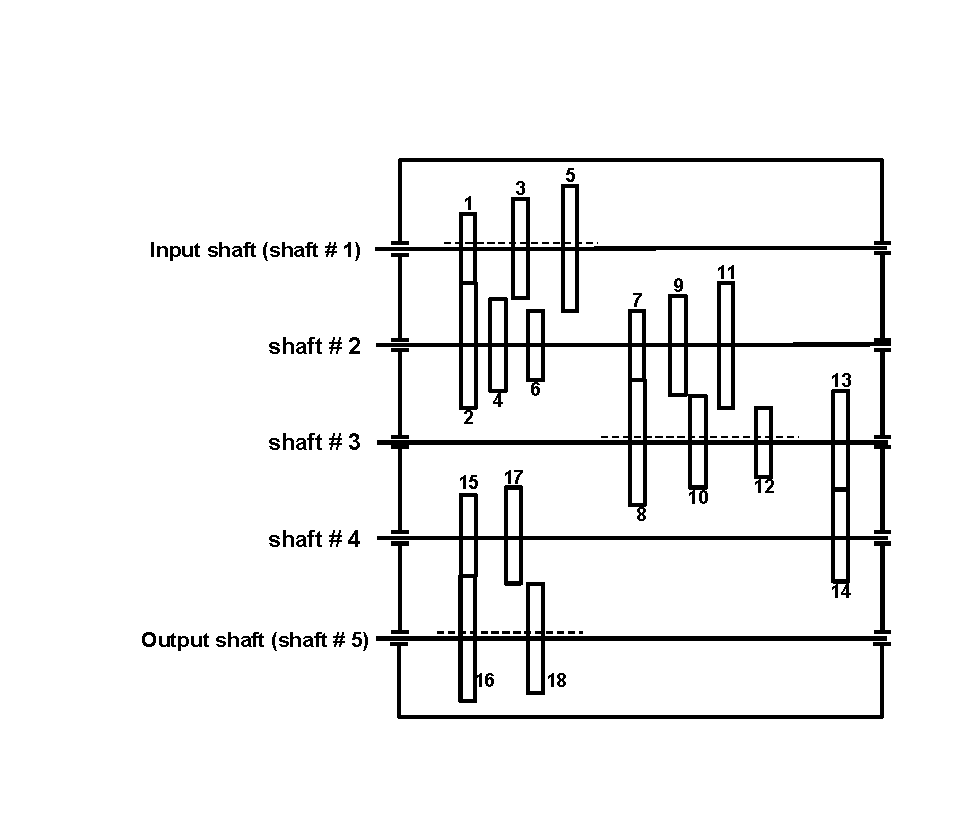
\includegraphics[width=80mm, height=65mm]{diagrams/geartrain.eps}}
 \caption{18-speed Gearbox layout. Gears in shafts 1, 3 and 5 can be
   translated to mesh with corresponding gears in shafts 2, 4 and 6
   respectively. With three different possible meshing of gears between
   shafts 1-2, 2-3 and two in shafts 2-4, 18 different output speeds are
   possible.}
 \label{geartrain}
\end{center}\end{figure}

A number of objectives can be considered for the design of the gear 
train design optimization, e.g.:
\begin{enumerate}[(i)]
\item minimization of the gear material used,
\item maximization of the power delivered, 
\item minimization of the error between desired and achieved output 
speeds.
\item minimization of the centre distance between input and output 
shaft,
\end{enumerate}
We will consider only the first three objectives in this study.

There are 29 variables over which an optimization problem can be defined:
\begin{enumerate}[(i)]
  \item thickness of gear-pairs, $t_i$ for $i = 1, 2, \dots 9$
  \item teeth module, the same for all the gear pairs,
  \item the power delivered $p$,
  \item the number of teeth in pinion of the $i^{th}$ gear-pair, 
  \item the number of teeth in wheel of the $i^{th}$ gear-pair, for $i = 1, 2, \dots 9$,
\end{enumerate}

To have varying number of teeth in the gears, the following 
constraints must be satisfied by all feasible gearbox designs:

\begin{enumerate}
  \item All mating gear-pairs on  two shafts should have the same 
   centre distances as the shaft distances.
  \item Since we have a two-dimensional gear-train layout, no gear 
   should interfere with any shaft.
  \item Maximum gear ratio in any gear pair should not exceed a limit
   $r^{max}$.
\end{enumerate}


% There are a large number of design parameters on which the optimization
% problem can be defined, depending on the aspects of the design we want to
% explore. 

The multi-objective formulation for the full problem is as follows:
\begin{singlespacing}
\begin{flushleft}


{\allowdisplaybreaks 
  \begin{align}
    \text{Maximize} \quad &f_1 =     \left. p,       \right.\\
    \text{Minimize} \quad &f_2 = \left. \frac{\pi m^2}{4} {\displaystyle\sum\limits_{i=1}^G {({n^2_{p_i}} + {n^2_{w_i}}) t_i }}\right.\\
    \text{Minimize} \quad &f_3 = \left. \max_{1 \le k \le 18}{|\Omega_k-{\Omega}_k^I|} \right. \\  
    \text{Subject to,}& \qquad  \left. \right.\nonumber \\
    &{\sigma}_{b_i} \leqslant  S_b \quad  &\left. \text{for} \quad i = 1, 2, \dots G, \right.\\
    &{\sigma}_{w_i} \leqslant S_w \quad   &\left. \text{for} \quad i = 1, 2, \dots G, \right.\\
    &t^{(L)} \leqslant t_i \leqslant t^{(U)}   &\left. \text{for} \quad i = 1, 2, \dots G, \right.\\
    &p^{(L)} \leqslant p \leqslant p^{(U)} \\
    \nonumber \\
    &n_1 + n_2 = n_3 + n_4 = n_5 + n_6,  \quad &\left. \text{(between shaft 1 and 2)} \right.\nonumber\\
    &n_7 + n_8 = n_9 + n_{10} = n_{11} + n_{12}, \quad &\left. \text{(between shaft 2 and 3)} \right.\nonumber\\
    &n_{15} + n_{16} = n_{17} + n_{18} \quad &\left. \text{(between shaft 4 and 5)} \right.\\
    \nonumber\\
    &n_2 \leqslant n_7 + n_8, \quad n_4 \leqslant n_7 + n_8, \nonumber\\
    &n_6 \leqslant n_7 + n_8, \quad n_7 \leqslant n_1 + n_2, \\
    \nonumber\\
    &n_9 \leqslant n_1 + n_2, \quad n_{11} \leqslant n_1 + n_2, \nonumber\\
    &n_8 \leqslant n_{13} + n_{14}, \quad n_{10} \leqslant n_{13} + n_{14},\\
    \nonumber\\
    &n_{12} \leqslant n_{13} + n_{14}, \quad n_{13} \leqslant n_7 + n_8, \nonumber\\
    &n_{14} \leqslant n_{15} + n_{16}, \quad n_{15} \leqslant n_{13} + n_{14},\\
    \nonumber\\
    &n_{17} \leqslant n_{13} + n_{14}\\
    \nonumber\\
    &\frac{n_{w_i}} {n_{p_i}}  \leqslant r^{max} \quad &\left. \text{(for i = 1, 2, \dots G)} \right.\nonumber\\
    &n_{w_i} \geqslant n^{(L)} &\left. \text{(for i = 1, 2, \dots G)} \right.\nonumber\\
    &n_{p_i} \geqslant n^{(L)} &\left. \text{(for i = 1, 2, \dots G)} \right.\nonumber\\
    &n_i \in \mathbb{Z} &\left. \text{(for i = 1, 2, \dots 2G)} \right. 
  \end{align}
}
Where, 

\end{flushleft}

\begin{itemize}
\item $m$ is the teeth module for all the gear pairs,
\item $n_{p_i}$ and $n_{w_i}$ are the number of teeth in the pinion 
and wheel in the $i^{th}$ gear-pair,
\item $t_i$ is the thickness of the gear-pair in cm., 
\item $\Omega_k$ is the actual $k^{th}$ output speed and $\Omega_k^I$ is the ideal $k^{th}$ output speed,
\item ${\sigma}_{b_i}$ is the bending stress developed in a gear-pair 
calculated as follows:

\begin{equation}
\sigma_{b_{i}} = \frac{97500 p { } k_c { } k_d { } (r_i + 1)} {a_{ i} { } {\omega}_{ i} { } t_{ i} { } m { } r_{ i} { } y_{ i} { } \text{cos} \beta} \\
\end{equation}

\item $S_b$ ($= 2,500\text{ kgf}/\text{cm}^2$) is the permissible bending stress,

\item ${\sigma}_{w_i}$ is the wearing stress developed in a gear-pair
calculated as follows:

\begin{equation}
\sigma_{w_{i}} = \frac{0.59 (r_i+1)}{r_i a_i} \sqrt{\frac{97500 p { } k_c { } k_d { } E (r_i + 1)}{ {\omega}_i t_i \text{sin} 2 \beta}}
\end{equation}
\item $S_w$ ($= 17,500\text{ kgf}/\text{cm}^2$) is the permissible wearing stress,

\item $k_c(=1.5)$ is the stress concentration factor,
\item $k_d(=1.1)$ is the dynamic load factor,
\item $r_i$ is the transmission ratio, defined as the ratio of number 
of teeth in the wheel $(n_{w_i})$ to the number of teeth in the 
pinion $(n_{p_i})$ for the $i^{th}$ gear-pair,
\item ${\omega}_i$ is the angular velocity of the wheel in rpm,
\item $a_i$ is the centre distance for the corresponding gear pair
given as 
\\
$a_i = \frac {m ( n_{w_i} + n_{p_i})} {2}$ , 
\item $y_i$ is the form load factor defined as 
$y_i = 0.52(1+ \frac{20}{n_{w_i}} )$ , 
\item ${\beta}(= 20 \text{ degrees})$ is the pressure angle,
\item $E $ ($= 2.1 \times 10^6\text{ kgf}/\text{cm}^2$) is the Young's modulus of the gear material. .
\end{itemize}

\end{singlespacing}

Here we will consider two instances of the problem:
\begin{enumerate}[(A)]
\item 11 variable problem in which thickness of all the gear-pairs and
  gear-module thickness are variable and only first two objectives are
  considered, and
\item the full problem.
\end{enumerate}

For the instance (A), the number of gear teeth layout is fixed to the
configuration given in table \ref{gearTeeth}. Constraints 3.8 onwards are
not applicable for this instance of the problem.

\begin{table}[!ht]
  \centering
  \begin{tabular}{|c|c|c|c|c|c|c|c|c|c|}
    \hline
    $i$ & 1 & 2 & 3 & 4 & 5 & 6 & 7 & 8 & 9  \\
    \hline
    \multicolumn{1}{|c|}{$n_{p_i}$} & 20 & 33 & 28 & 32 & 34 & 33 & 33 & 20 & 26\\
    \hline
    \multicolumn{1}{|c|}{$n_{w_i}$} & 56 & 43 & 48 & 37 & 35 & 36 & 34 & 54 & 48\\
    \hline
  \end{tabular}
  \caption{No. of teeth for each gear-pair in fixed layout gear-train design.}
  \label{gearTeeth}
\end{table}





\subsection{NSGA-II formulation and the pareto-front}
We use the same NSGA-II formulation as in \citep{debgt} to obtain the
pareto-optimal solutions. For the 11 variables case we fix the 
gear-box layout by fixing the number of teeth in each gear to the 
values shown in table \ref{gearTeeth}. 



In second case we utilize the equality constraints given in equations 3.4
to eliminate five gear teeth variables. We code the gear teeth variables in
such a way so as to avoid evaluating permutations of same combinations of
gears in each transmission stage. Also, we condense similar constraints
into one constraint wherever possible. The probabilities of recombination
and mutation operator are 0.9 and 0.3 respectively for both the
optimization cases. For the 11 variables optimization, we run NSGA-II for
600 generations with a population size of 3000, and for 10000 generations
with 3000 initial population for the 29 variable case. NSGA-II yields 927
points in the pareto-front for the first case. The pareto-front for the 29
variables optimization has 989 points. The pareto-fronts are shown in
figures \ref{gt11Clusters} and \ref{gtvClusters}.


\section{Fixed transmission ratio problem}

Figure \ref{gt11rv} shows the Isomap residual variances for the
pareto-front of the fixed lay-out gearbox pareto-front. The largest drop in
the Isomap residual variance from 3 to 4 dimensional Isomap embedding. This
suggests the pareto-front may have an intrinsic dimensionality of four, and
we can expect to have clusters of dimensions lower than 4.

The PCA explained variance is shown in \ref{gt11ev}, which clearly shows
that the pareto-front is one dimensional in the parameter space. Table
\ref{first2GTPCs} shows the weights of five variables which have the
highest absolute component in in the first two principal components. The
thicknesses of the gear pairs in the final transmission stage are the
variables with the highest weight in the first principal component. Next
are the thickness of the second and fifth gear-pairs. In the second
principal component, the gear module is the most important
variable. Weights of all the other variables are  negligible in this
principal component.


% \begin{figure}[ht]\begin{center}
%  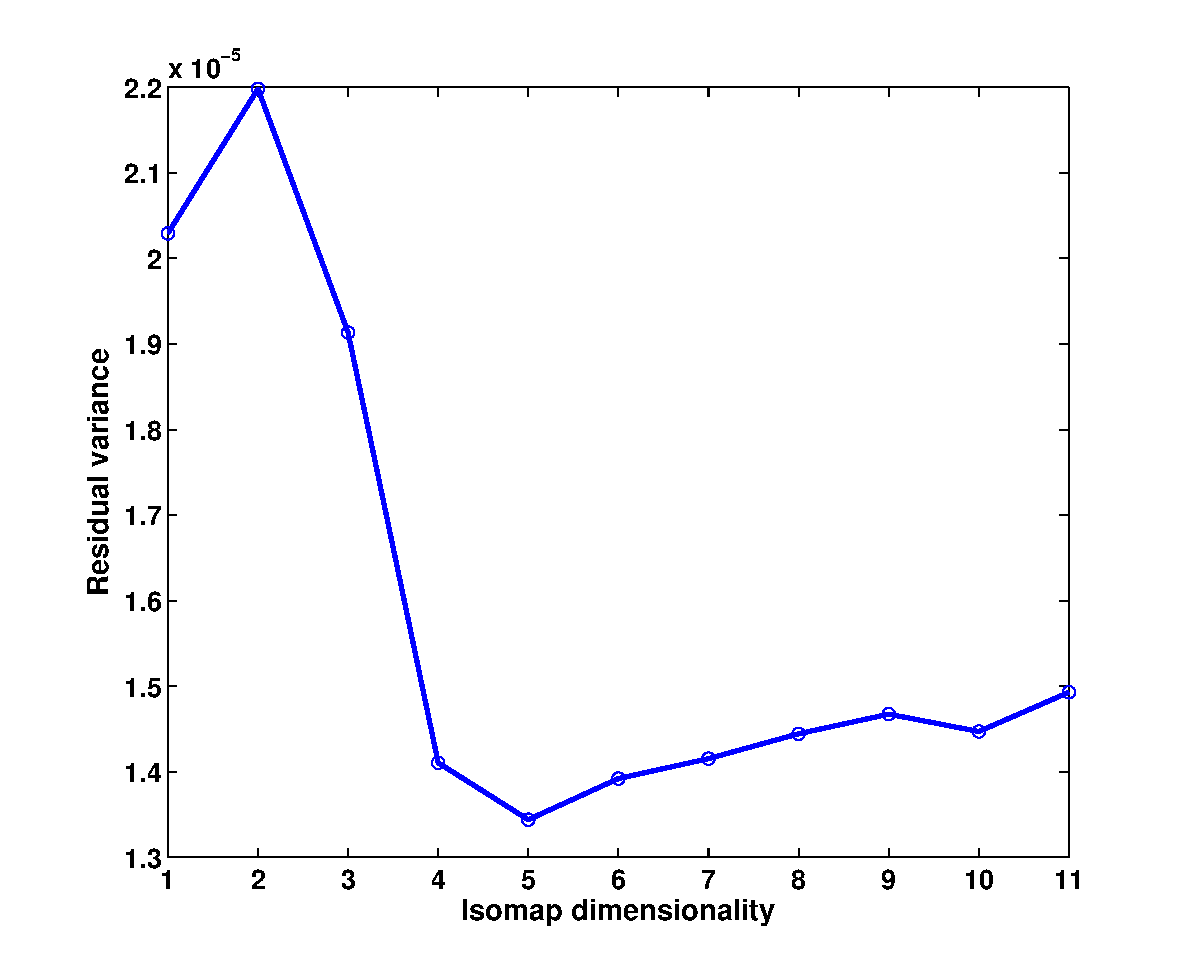
\includegraphics[width=100mm, height=80mm]{dia/gt11rv.eps}
%  \caption{Isomap residual variance for the fixed lay-out paret-front}
%  \label{gt11rv}
% \end{center}\end{figure}

\begin{figure}[ht]\begin{center}
 \subfloat[Isomap Residual Variance. ]{
 \label{gt11rv} 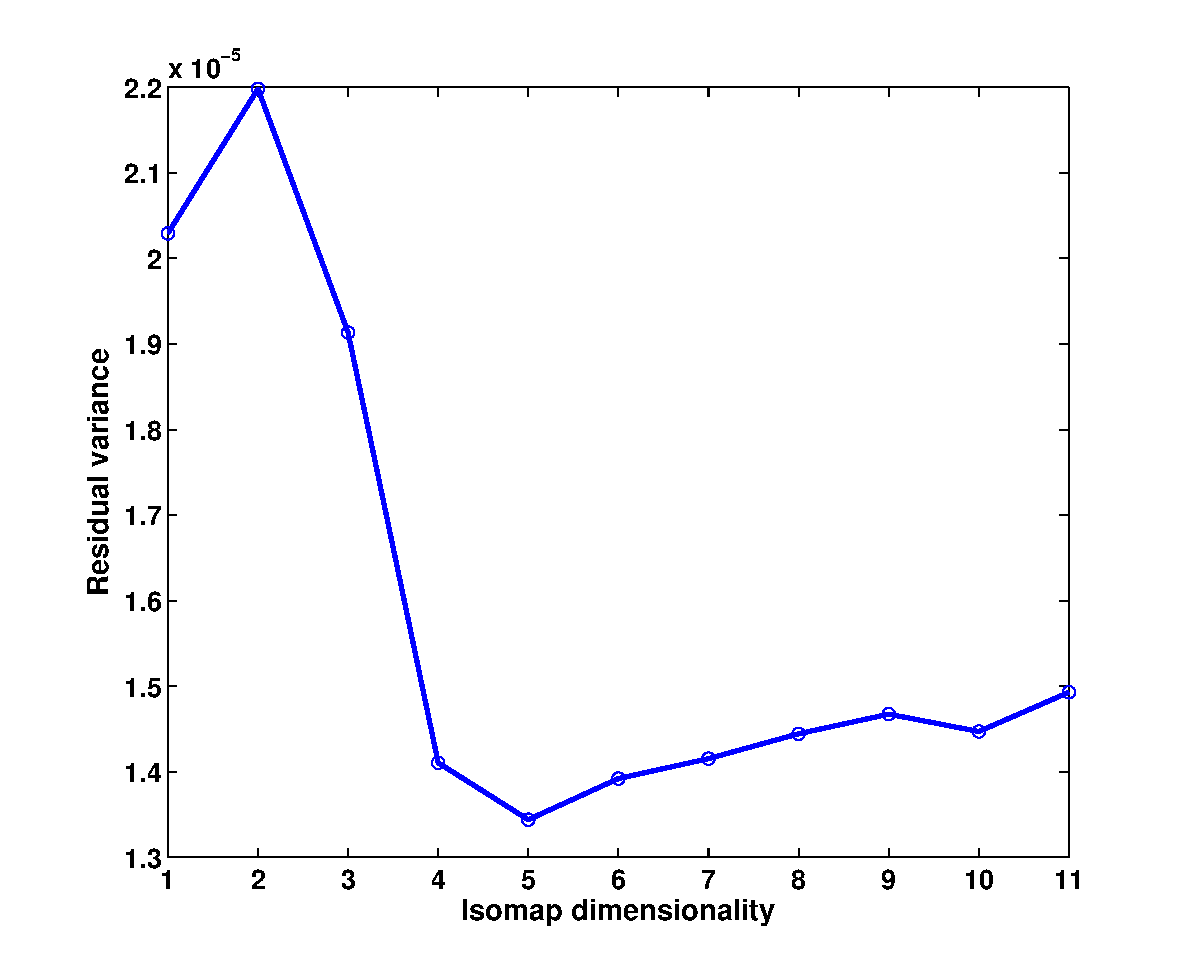
\includegraphics[width=62mm, height=52mm]{dia/gt11rv.eps}}
 \subfloat[PCA Explained variance.]{
 \label{gt11ev} 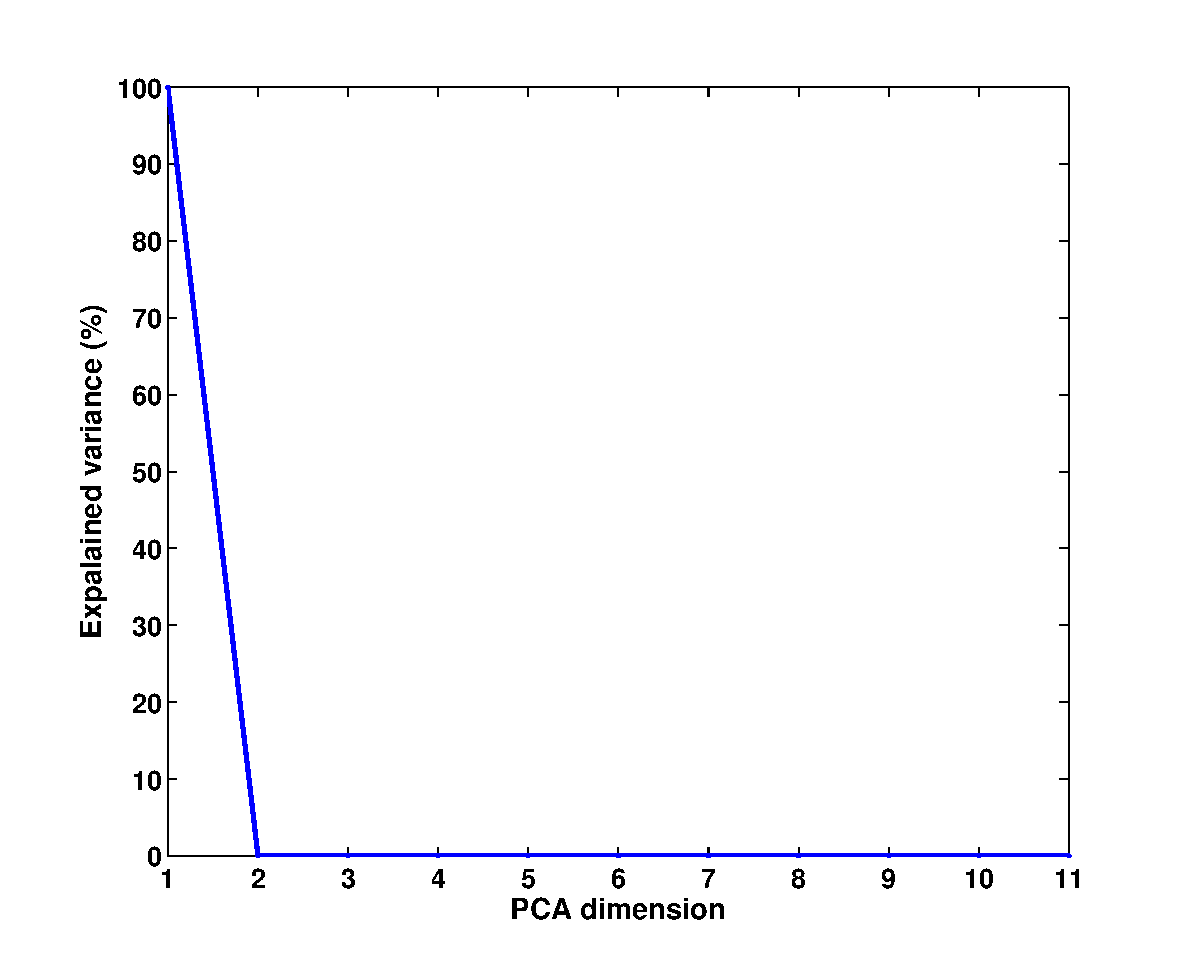
\includegraphics[width=62mm, height=52mm]{dia/gt11ev.eps}}
\caption{Isomap and PCA results for the fixed lay-out problem. The largest
  drop in residual variance is for the four dimensional Isomap
  embedding. The explained variance plot shows only one significant
  component.}
 \label{gt11rv}
\end{center}\end{figure}
 
\begin{table}[!ht]
  \centering
  \begin{tabular}{|c|c|c|c|c|c|}
    \hline
    \multirow{2}{*}{First PC}   & ($t_9$) &  ($t_8$) &  ($t_7$)  & ($t_6$) & ($p$)\\
    & -0.8444  & -0.4617  & 0.1837 & -0.1511 & 0.0733  \\
    \hline
    \multirow{2}{*}{Second PC}   & ($m$) &  ($t_5$) &  ($t_6$)  & ($t_9$) & ($t_8$)\\
    & 0.9997 & -0.0124 & 0.0097 & 0.0087 &  0.0087 \\
    \hline
  \end{tabular}
  \caption{First two principal components of the fixed layout gearbox pareto-front. $t_9$ and $t_8$ are the variables with the highest weights in the first component.}
  \label{first2GTPCs}
\end{table}

\subsection{Clustering the pareto-front}
Although it is possible to cluster the pareto-front into smaller clusters
by varying the $k$ parameter in our algorithm, we show and analyze
significantly sized and smaller number of clusters for the sake of
simplicity. Figure \ref{gt11Clusters} shows the 11 clusters obtained by
setting $k = 6.0$.

\begin{figure}[ht]\begin{center}
 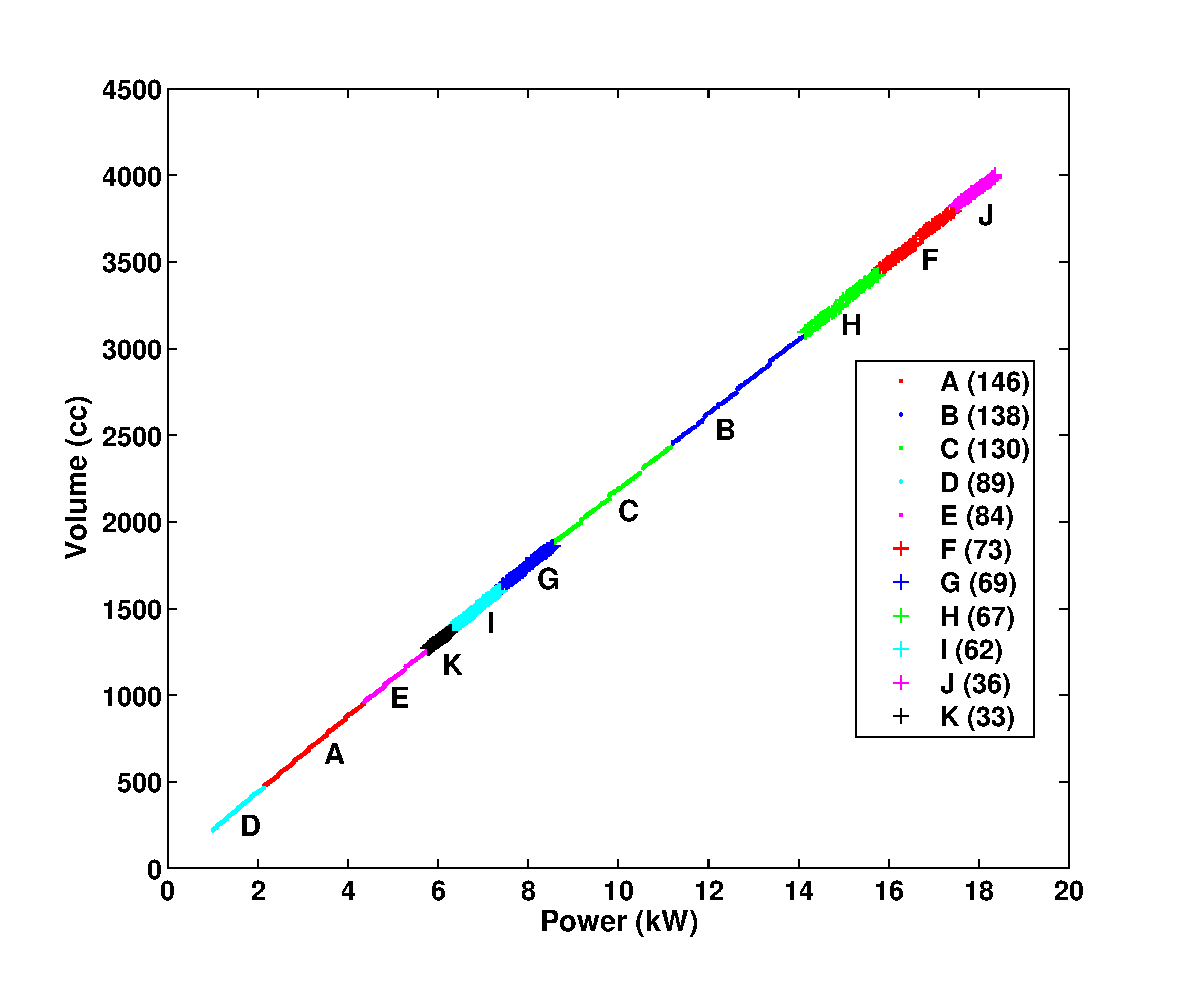
\includegraphics[width=100mm, height=80mm]{dia/gt11cpareto1.eps}
 \caption{Fixed layout gearbox design pareto-front and clusters in the
   objective space. There are 927 solutions in the pareto-front. The
   clusters in the extremes of the pareto-front are small.}
 \label{gt11Clusters}
\end{center}\end{figure}

\subsubsection{Isomap and PCA analysis}

The Isomap residual variance for most of the clusters is negligible except
for the cluster \textbf{D} for the residual variance is plotted in figure
\ref{gt11clustersrv}. The largest drop in residual variance is observed for
the second Isomap dimension after which it is constant, suggesting a
manifold dimensionality of one. All the clusters thus have a manifold
dimensionality of one, conforming to the {\em chunk dimensionality
  conjecture}. PCA analysis shows that clusters \textbf{B}, \textbf{C},
\textbf{F}, \textbf{J} and \textbf{K} are clearly one dimensional with the
first principal component of these clusters having explained variance of
more than 99\%. For the cluster \textbf{D}, the first principal component
has an explained variance of 80\% while the second principal component has
20\%. Figure \ref{gt11ev} shows the explained variance plot of cluster
\textbf{D} along with other clusters whose first components have explained
variance less than 99\%.

 



\begin{figure}[ht]\begin{center}
    \subfloat[Isomap Residual Variance for the cluster \textbf{D}.]{
      \label{gt11clustersrv} 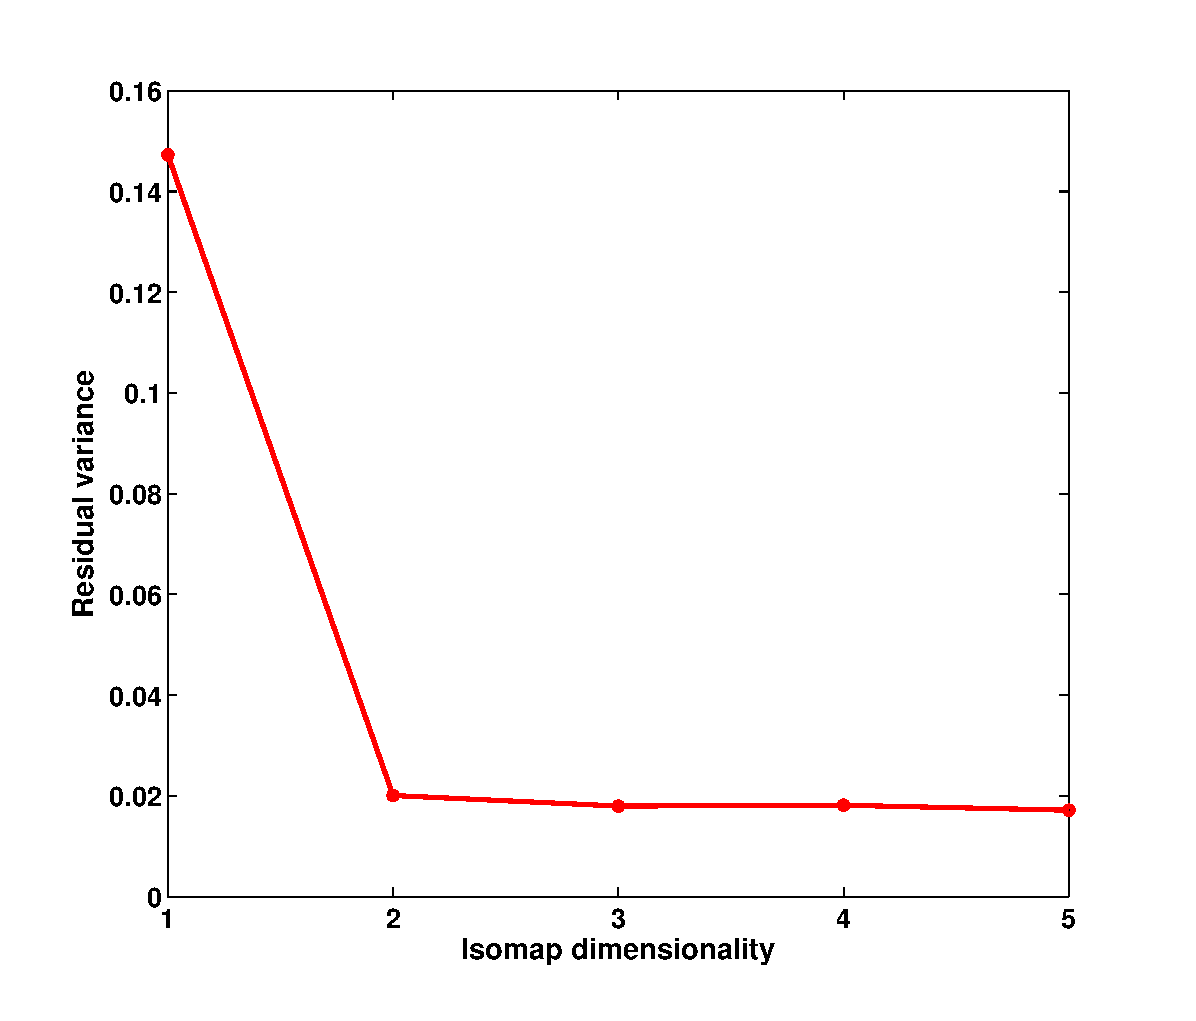
\includegraphics[width=62mm, height=52mm]{dia/gt11cluster4rv.eps}}
    \subfloat[PCA Explained variance for some of the clusters.]{
      \label{gt11clustersev} 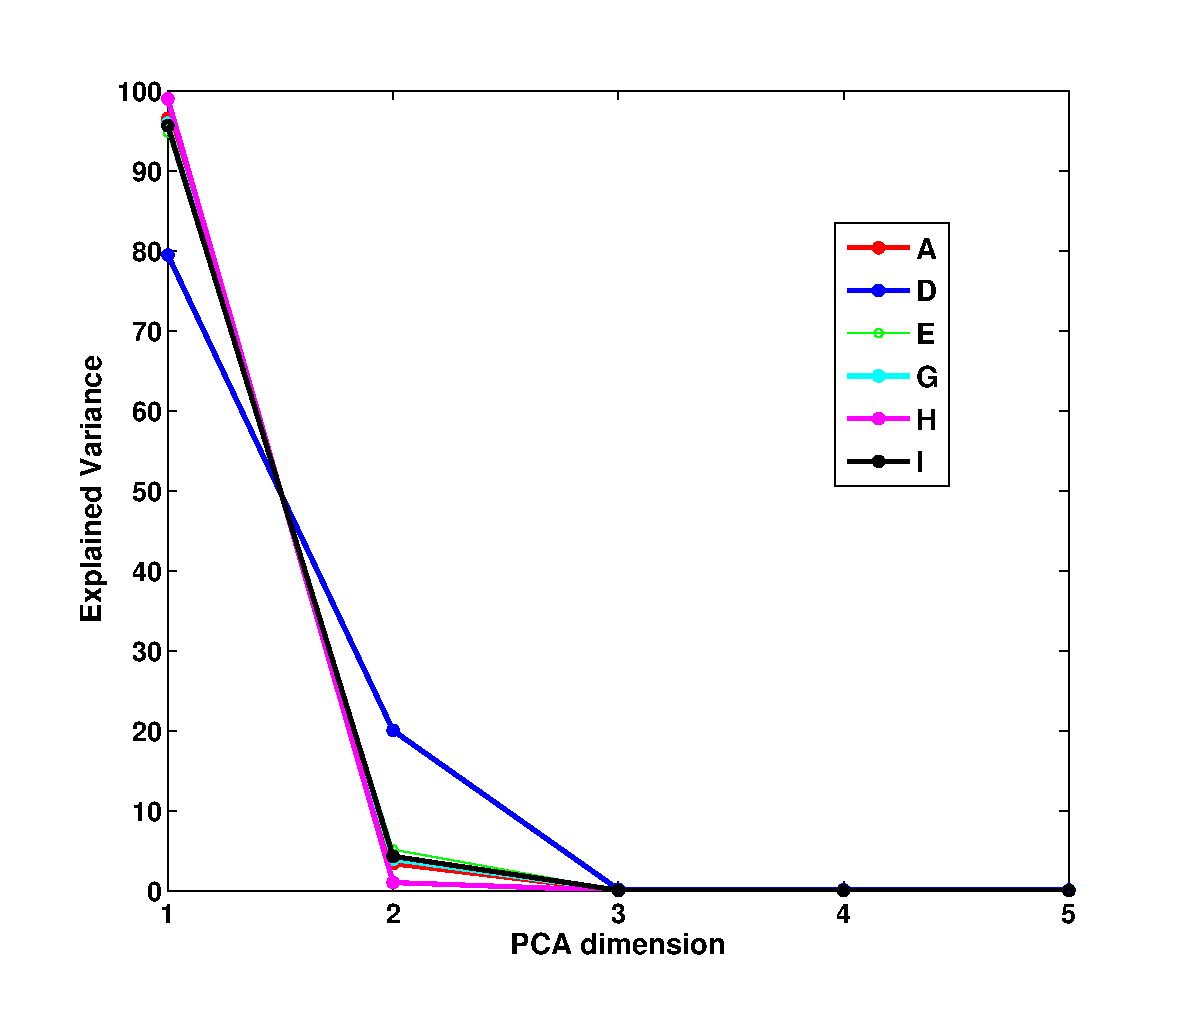
\includegraphics[width=62mm, height=52mm]{dia/gt11clustersEV.eps}}
    \caption{Isomap and PCA results for the clusters of fixed lay-out
      problem. \textbf{D} has the largest residual variance, all other
      clusters have negligible residual variances. The plot indicates a one
      dimensional manifold. Only cluster \textbf{D} has two significant
      principal component, all others have only one significant principal
      component.}
    \label{gt11clustersVar}
  \end{center}
\end{figure}


{\tiny

  {\small
    \begin{table}[!ht]
      \centering
      \begin{tabular}{|c|c|c|c|c|c|c|c|c|c|c|c|}
        \hline
        \multirow{2}{*}{\textbf{A}}   & $p$ & \cellcolor[gray]{0.45} $t_8$ & \cellcolor[gray]{0.50} $t_9$  & $m$ & \cellcolor[gray]{0.65} $t_7$ & \cellcolor[gray]{0.60} $t_4$ & \cellcolor[gray]{0.70} $t_5$ & \cellcolor[gray]{0.75} $t_6$ & \cellcolor[gray]{0.40} $t_1$ & \cellcolor[gray]{0.80} $t_3$ & \cellcolor[gray]{0.55} $t_2$ \\
        & 0.99  & 0.04  & 0.02 & 0.02 & 0.01 & 0.01 & 0.01 & 0.01 & 0.00 & 0.00 & 0.00 \\
        \hline
        \multirow{2}{*}{\textbf{B}}   & $p$ & \cellcolor[gray]{0.45} $t_8$ &  $m$  & \cellcolor[gray]{0.50}$t_9$ & \cellcolor[gray]{0.65} $t_7$ & \cellcolor[gray]{0.60} $t_4$ & \cellcolor[gray]{0.70} $t_5$ & \cellcolor[gray]{0.75} $t_6$ & \cellcolor[gray]{0.40} $t_1$ & \cellcolor[gray]{0.80} $t_3$ & \cellcolor[gray]{0.55} $t_2$ \\
        & 0.99 & 0.01 & 0.01 & 0.01 &  0.00 & 0.00 & 0.00 & 0.00 & 0.00 & 0.00 & 0.00 \\
        \hline
        \multirow{2}{*}{\textbf{C}} & $p$ & \cellcolor[gray]{0.45} $t_8$ & \cellcolor[gray]{0.50} $t_9$ &  $m$ & \cellcolor[gray]{0.65} $t_7$ & \cellcolor[gray]{0.60} $t_4$ & \cellcolor[gray]{0.70} $t_5$ & \cellcolor[gray]{0.75} $t_6$ & \cellcolor[gray]{0.40} $t_1 $ & -- & -- \\
        & 0.99 & 0.02 & 0.01 & 0.01 & 0.01 & 0.01 & 0.01 & 0.01 & 0.01 & 0 & 0 \\
        \hline
        \multirow{4}{*}{\textbf{D}} & $p$ & \cellcolor[gray]{0.45} $t_8$ & \cellcolor[gray]{0.50} $t_9$ &  \cellcolor[gray]{0.65} $t_7$ & $m$ & \cellcolor[gray]{0.60} $t_4$ & \cellcolor[gray]{0.70} $t_5$ & \cellcolor[gray]{0.75} $t_6$ &\cellcolor[gray]{0.40} $t_1$ &\cellcolor[gray]{0.80} $t_3$ & \cellcolor[gray]{0.55} $t_2$ \\
        & 0.99 & 0.07 & 0.06 & 0.03 & 0.03 & 0.03 & 0.03 & 0.02 & 0.02 & 0.00 & 0.00 \\ 
        \cline{2-12}
        & \cellcolor[gray]{0.45} $t_8$ & \cellcolor[gray]{0.50} $t_9$ & \cellcolor[gray]{0.65} $t_7$ &  \cellcolor[gray]{0.60} $t_4$ & \cellcolor[gray]{0.70} $t_5$ & \cellcolor[gray]{0.75} $t_6$ & \cellcolor[gray]{0.40} $t_1$ & $p$ & $m$ & \cellcolor[gray]{0.80} $t_3$ & \cellcolor[gray]{0.55} $t_2$ \\
        & -0.64 & -0.46 & -0.32 & -0.29 & -0.26 & -0.24 & 0.17 & 0.12 & 0.02 & 0.00 & 0.00 \\
        \hline
        \multirow{2}{*}{\textbf{E}} & $p$ & \cellcolor[gray]{0.45} $t_8$ & \cellcolor[gray]{0.50} $t_9$ &  \cellcolor[gray]{0.65} $t_7$ & \cellcolor[gray]{0.70} $t_5$ & \cellcolor[gray]{0.60} $t_4$ & \cellcolor[gray]{0.75} $t_6$ & $m$ & \cellcolor[gray]{0.40} $t_1$ & \cellcolor[gray]{0.80} $t_3$ & \cellcolor[gray]{0.55} $t_2$ \\
        & 0.99 & 0.07 & 0.05 & 0.03 & 0.02 & 0.02 & 0.02 & 0.01 & 0.01 & 0.00 & 0.00 \\ 
        \hline
        \multirow{2}{*}{\textbf{F}} & $p$ & \cellcolor[gray]{0.45} $t_8$ & \cellcolor[gray]{0.50} $t_9$ &  \cellcolor[gray]{0.65} $t_7$ & \cellcolor[gray]{0.60} $t_4$ & \cellcolor[gray]{0.75} $t_6$ & \cellcolor[gray]{0.70} $t_5$ & \cellcolor[gray]{0.40} $t_1$ & $m$ & \cellcolor[gray]{0.55} $t_2$ & \cellcolor[gray]{0.80} $t_3$ \\
        & 0.99 & 0.03 & 0.02 & 0.01 & 0.01 & 0.01 & 0.01 & 0.01 & 0.0 & 0.0 & 0.0 \\ 
        \hline
        \multirow{2}{*}{\textbf{G}} & $p$ & \cellcolor[gray]{0.45} $t_8$ & \cellcolor[gray]{0.50} $t_9$ & \cellcolor[gray]{0.65} $t_7$ & \cellcolor[gray]{0.75} $t_6$ & \cellcolor[gray]{0.60} $t_4$ & \cellcolor[gray]{0.70} $t_5$ & \cellcolor[gray]{0.40} $t_1$ & $m$ & \cellcolor[gray]{0.80} $t_3$ & \cellcolor[gray]{0.55} $t_2$ \\
        & 0.99 & 0.07 & 0.05 & 0.04 & 0.03 & 0.03 & 0.03 & 0.02 & 0.01 & 0.0 & 0.0 \\ 
        \hline
        \multirow{2}{*}{\textbf{H}} & $p$ & \cellcolor[gray]{0.45} $t_8$ & \cellcolor[gray]{0.50} $t_9$ & \cellcolor[gray]{0.60} $t_4$ &\cellcolor[gray]{0.65} $t_7$ &\cellcolor[gray]{0.70} $t_5$ &\cellcolor[gray]{0.75} $t_6$ &\cellcolor[gray]{0.40} $t_1$ & $m$ & -- & -- \\
        & 0.99 & 0.04 & 0.03 & 0.02 & 0.01 & 0.01 & 0.01 & 0.01 & 0.00 & 0 & 0 \\ 
        \hline
        \multirow{2}{*}{\textbf{I}} & $p$ &\cellcolor[gray]{0.45} $t_8$ & \cellcolor[gray]{0.50} $t_9$ & \cellcolor[gray]{0.65} $t_7$ &\cellcolor[gray]{0.60} $t_4$ &\cellcolor[gray]{0.70} $t_5$ &\cellcolor[gray]{0.75} $t_6$ &\cellcolor[gray]{0.40} $t_1$ & $m$ & -- & -- \\
        & 0.98 & 0.10 & 0.07 & 0.05 & 0.04 & 0.04 & 0.04 & 0.03 & 0.01 & 0 & 0 \\ 
        \hline
        \multirow{2}{*}{\textbf{J}} & $p$ &\cellcolor[gray]{0.45} $t_8$ &\cellcolor[gray]{0.50} $t_9$ & \cellcolor[gray]{0.65} $t_7$ & \cellcolor[gray]{0.60} $t_4$ &\cellcolor[gray]{0.75} $t_6$ &\cellcolor[gray]{0.70} $t_5$ &\cellcolor[gray]{0.40} $t_1$ &\cellcolor[gray]{0.80} $t_3$ &\cellcolor[gray]{0.55} $t_2$ & $m$ \\
        & 0.97 & 0.13 & 0.10 & 0.06 & 0.06 & 0.05 & 0.05 & 0.03 & 0.0 & 0.0 & 0 \\ 
        \hline
        \multirow{2}{*}{\textbf{K}} & $p$ &\cellcolor[gray]{0.45} $t_8$ & \cellcolor[gray]{0.50} $t_9$ & \cellcolor[gray]{0.65} $t_7$ &\cellcolor[gray]{0.60} $t_4$ &\cellcolor[gray]{0.70} $t_5$ &\cellcolor[gray]{0.75} $t_6$ &\cellcolor[gray]{0.40} $t_1$ &\cellcolor[gray]{0.80} $t_3$ &\cellcolor[gray]{0.55} $t_2$ & $m$ \\
        & 0.85 & 0.33 & 0.25 & 0.17 & 0.14 & 0.13 & 0.13 & 0.09 & -0.00 & -0.00 & 0 \\ 
        \hline
      \end{tabular}
      \caption{Principal component weights of each cluster in sorted order of absolute weights. Background shading indicates the input to output speeds for the gear pair. Darker cells indicate higher ratio. The gear pairs in the last transmission stage have the highest weights and those in the first transmission stage have the lowest weights for all the clusters.}
      \label{gt11pcTopWeights}
    \end{table}
  }
}
% & $t_$ & $t_$ & $t_$ & $t_$ & $t_$ & $t_$ 
% & 0.0 & 0.0 & 0.0 & 0.0 & 0.0 & 0.0 

Table \ref{gt11pcTopWeights} shows the top weights of the principal
components of the clusters. Only the first principal components for most of
the clusters are shown, as most of them have negligible explained variances
for subsequent principal components. Power is the predominant variable in
the principal components of all the clusters, followed by thickness of the
gear-pairs in the final transmission stage.  In larger clusters, module
occupies higher positions compared to smaller clusters.


\subsection{Discussion}
Apart from being a variable, power ($p$) is also one of the objectives of
the multi-objective optimization problem, taking a different value for each
pareto-optimal solution. This explains its highest weight in the principal
components of all the clusters. Next we have the thicknesses of gear-pairs
($t_i$) with module thickness ($m$) occupying various positions depending
on the size of the clusters. The positions of the thickness variables can
be explained on the basis of input to output speed ratio for each
gear-pair.  These ratios are shown in table \ref{iosRatio} in increasing
order. The gear-pairs having smaller input to output speed ratio should
have higher thickness as the pinion of these gear-pairs has to withstand
higher stresses.  The speed of the gear-pairs also inversely affects the
stress, the higher the speed the lower will be the stress for the same
power transmitted.



\begin{table}[!ht]
  \centering
  \begin{tabular}{|c|c|c|c|c|c|c|c|c|c|}
    \hline
    Gear pair No. & \cellcolor[gray]{0.40} 1 & \cellcolor[gray]{0.45} 8 & \cellcolor[gray]{0.50} 9 & \cellcolor[gray]{0.55} 2 & \cellcolor[gray]{0.60} 4 & \cellcolor[gray]{0.65} 7 & \cellcolor[gray]{0.70} 5 &\cellcolor[gray]{0.75} 6 & \cellcolor[gray]{0.80} 3\\
    \hline
    I/O Speed ratio & \cellcolor[gray]{0.40} 0.35 & \cellcolor[gray]{0.45} 0.46 & \cellcolor[gray]{0.50} 0.54 & \cellcolor[gray]{0.55} 0.76 & \cellcolor[gray]{0.60} 0.86 & \cellcolor[gray]{0.65} 0.97 & \cellcolor[gray]{0.70}0.97 & \cellcolor[gray]{0.75} 1.09 & \cellcolor[gray]{0.80} 1.71\\
    \hline
  \end{tabular}
  \caption{Gear pairs with lowest input to output speed ratios.}
  \label{iosRatio}
\end{table}


The positions of thickness variables in the principal components in table
\ref{gt11pcTopWeights} have been colour coded similar to table
\ref{iosRatio}. It can be observed that the thickness variables occur in
the order of the transmission stage they are in. $t_8$ and $t_9$ are the
thicknesses of the gears in the final transmission stage, $t_7$ in the
penultimate stage followed by $t_4$, $t_5$, $t_6$ and $t_1$, $t_2$, $t_3$
in the second and first stages.  The speeds would generally be the lowest
in the final transmission stage, consequently, the thicknesses in these
gear-pairs would have to be increased commensurate with the increasing
power. As opposed to this, the shafts in the first transmission stage will
have the highest speeds and the stresses will be the lowest, hence the
thickness of these gears generally stick to the lowest possible value of
0.5. Only for high power gear boxes do they show any variation, e.g.  in
clusters \textbf{J} and \textbf{F}, in which $t_1$ has higher absolute
weights than module ($m$). It can also be noticed that gear-pairs in the
same shaft are arranged in the order of increasing input to output ratio in
the principal components. Although $G_1$ has the lowest input to output
speed ratio, the position of $t_1$ in the principal components is after the
gear-pairs in other transmission stages. This suggests that the speed of
the gear pair is an important factor in stress and thickness of the
gear-pair.


\begin{figure}[ht]\begin{center}
 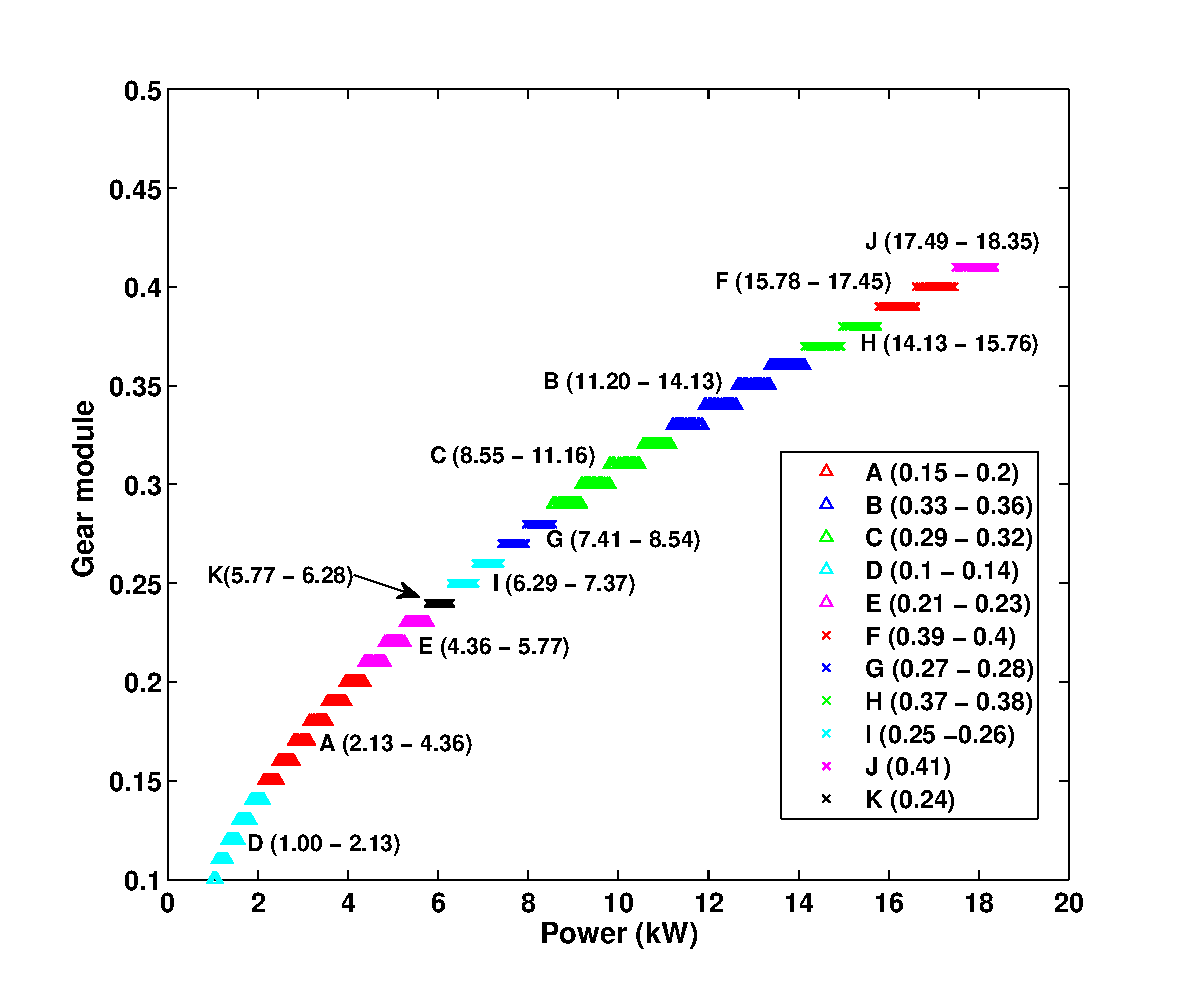
\includegraphics[width=100mm, height=80mm]{dia/gt11pVsm.eps}
 \caption{Power Vs. module characteristics of the pareto-front. Clusters occupy contiguous steps in the staircase structure.}
 \label{gt11pVsm}
\end{center}\end{figure}

Module weight in the principal components depends upon the size of the
cluster. For clusters \textbf{A}, \textbf{B}, \textbf{C} and \textbf{D},
$m$ occurs at positions up to fifth.  Figure \ref{gt11pVsm} shows the power
Vs. module plot for the clusters.  The staircase structure of this plot
shows that for a higher power gearbox a larger module is required. This
plot also explains the higher weights of $m$ variable in the clusters
mentioned earlier.  The cluster \textbf{A} is composed of designs with
five different module widths, cluster \textbf{B} and \textbf{C} with four,
and cluster \textbf{D} again with five different module widths. For these
clusters, module has a good range of variation hence the higher weights in
the principal components. On the other hand, clusters \textbf{J} and
\textbf{K} have designs with the same module width, their principal
components indicate this by having zero weights for $m$.




\section{29 Variable problem}

The pareto-front and the clusters obtained for the 29 variable problem
are shown in the figure \ref{gtvClusters}. As with the fixed layout problem,
we keep the size and number of clusters low by choosing a higher $k$ parameter 
value in our algorithm.


\begin{figure}[ht]\begin{center}
 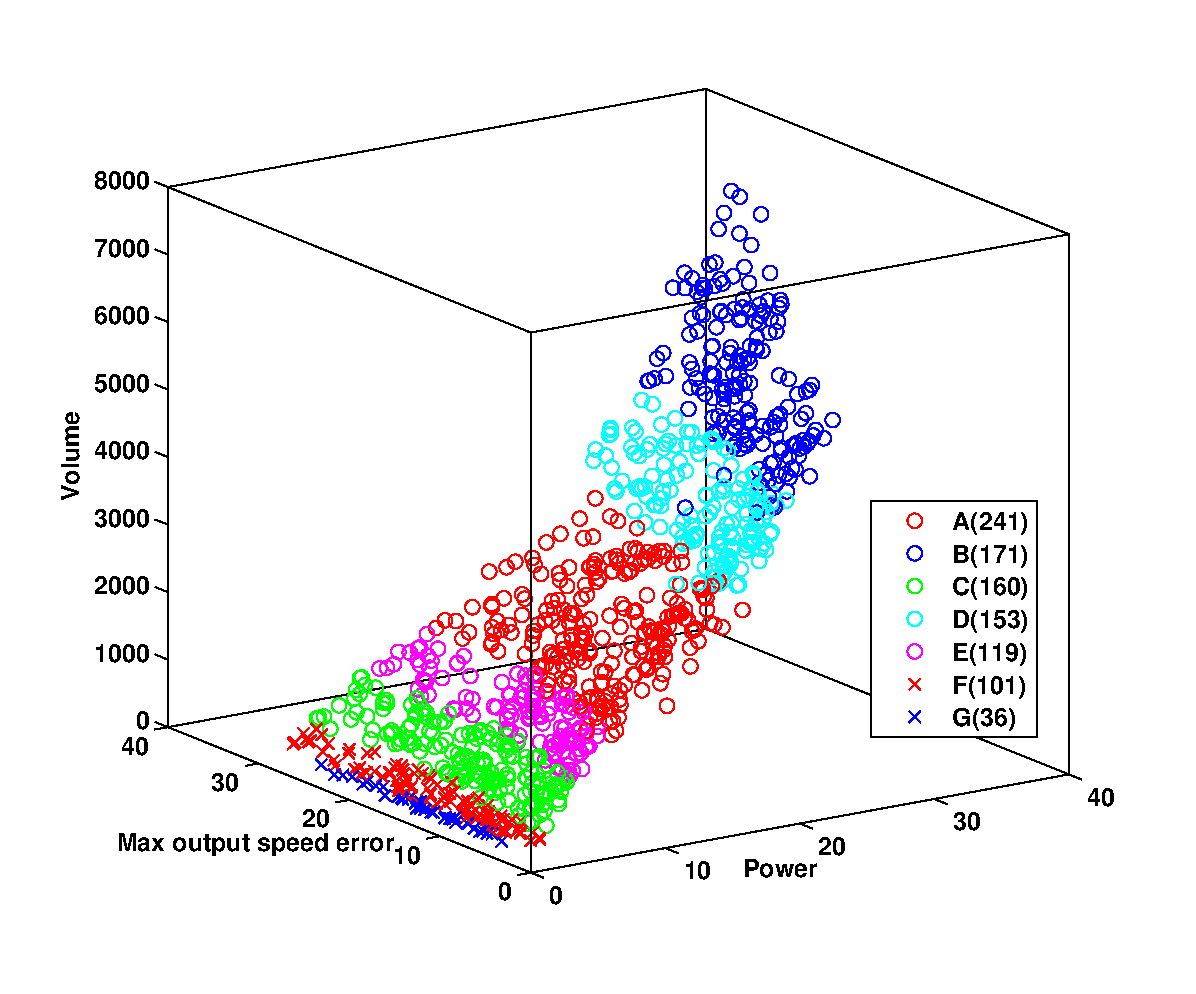
\includegraphics[width=100mm, height=80mm]{dia/gtvopareto2.eps}
 \caption{The pareto-front and the clusters for the 29-variable problem. The pareto-front manifold is clearly a two dimensional manifold in the objective space. }
 \label{gtvClusters}
\end{center}\end{figure}

Figure \ref{gtvRvEv} shows the Isomap residual variance and PCA explained
variances for the pareto-front. The residual variance plot gives no certain
indications about the dimensionality of the pareto-front. The largest drop
in residual variance occurs for second Isomap dimension and keeps dropping
up-to the fifth dimension after which it flattens out. The explained
variance also gives a similar picture; the explained variances for the
first, second, third and fourth principal components are 63.6\%, 11.6\%,
7.6\% and 7.1\% respectively. 


\begin{figure}[ht]\begin{center}
    \subfloat[Isomap Residual Variance.]{
      \label{gt11rv} 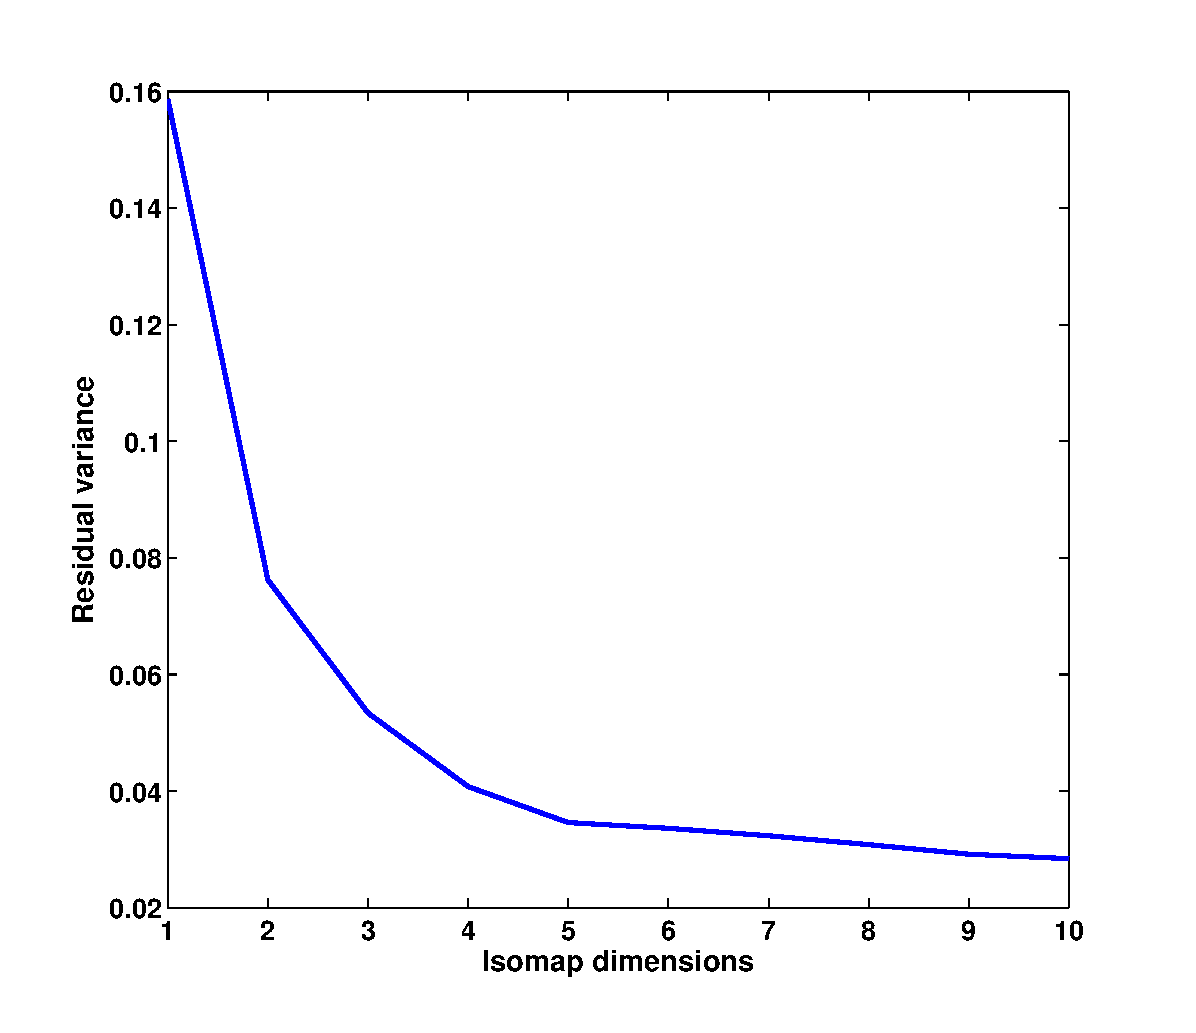
\includegraphics[width=62mm, height=52mm]{dia/gtvorv1.eps}}
    \subfloat[PCA explained variance.]{
      \label{gt11ev} 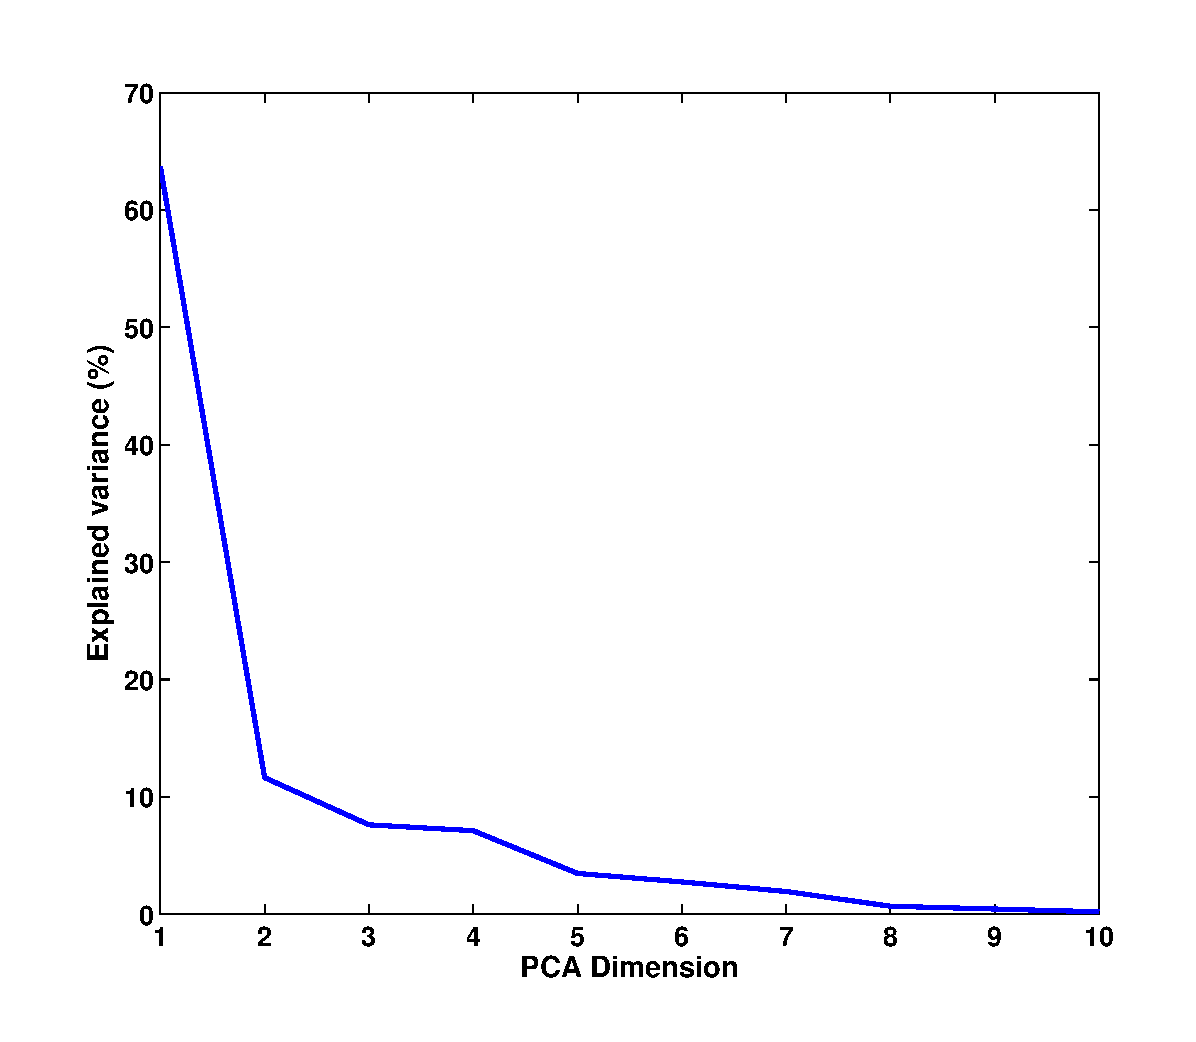
\includegraphics[width=62mm, height=52mm]{dia/gtvWholeEV.eps}}
    \caption{Isomap and PCA results for the 29 variable gearbox design
      problem pareto-front. Although the largest drop in residual variance
      is for two-dimensional embedding, it keeps dropping up to the fifth
      dimension. PCA explained variance shows four significant principal
      components.}
    \label{gtvRvEv}
  \end{center}
\end{figure}


Table \ref{first4GTVPCs} shows the variables with highest absolute weights
of first four principal components. There are no predominant variables in
the principal components, the weights are somewhat evenly distributed for
the first principal component. The second principal component, however, is 
dominated by the $p$ variable followed by gear teeth variables.


\begin{table}[!ht]
  \centering
  \begin{tabular}{|c|c|c|c|c|c|}
    \hline
    \multirow{2}{*}{First PC}   & $n_{16}$ &  $t_{5}$ &  $n_{8}$  & $n_{10}$ & $n_3$\\
    & 0.35  & 0.29  & 0.29 & 0.29 & 0.26  \\
    \hline
    \multirow{2}{*}{Second PC}   & $p$ &  $n_{2}$ &  $n_{16}$  & $n_{18}$ & $n_8$\\
    & -0.81 & -0.27 & -0.22 & -0.21 &  0.16 \\
    \hline
    \multirow{2}{*}{Third PC}   & $n_{11}$ &  $n_{9}$ &  $n_{5}$  & $n_{7}$ & $n_{3}$\\
    & -0.43 & -0.41 & 0.41 & -0.40 & 0.38 \\
    \hline
    \multirow{2}{*}{Fourth PC}   & $n_{12}$ &  $n_{10}$ &  $n_{8}$  & $n_{2}$ & $n_{4}$\\
    & 0.41 & 0.41 & 0.41 & -0.37 &  -0.33 \\
    \hline
  \end{tabular}
  \caption{Highest absolute weights of the first four principal components 
    of the gear train design problem (29 variables). There is no 
    dominant variable in the first principal component.}
  \label{first4GTVPCs}
\end{table}




\subsection{Analysis of the clusters}
 

\begin{figure}[ht]\begin{center}
 \subfloat[Clusters \textbf{A}, \textbf{C} and \textbf{E}.]{
 \label{gt11rv} 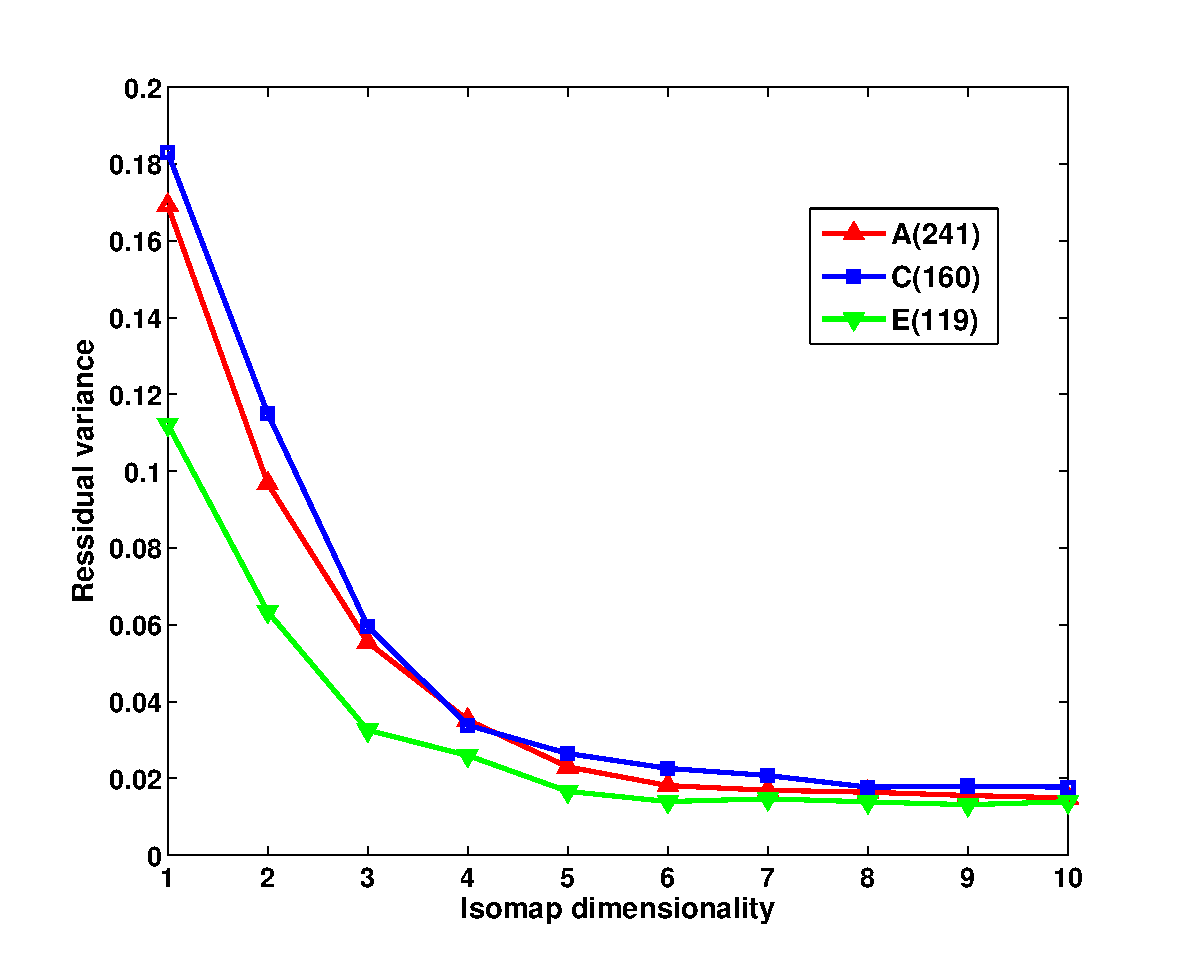
\includegraphics[width=62mm, height=52mm]{dia/gtvcrv1.eps}}
 \subfloat[Clusters \textbf{B}, \textbf{C}, \textbf{E} and \textbf{F}]{
 \label{gt11ev} 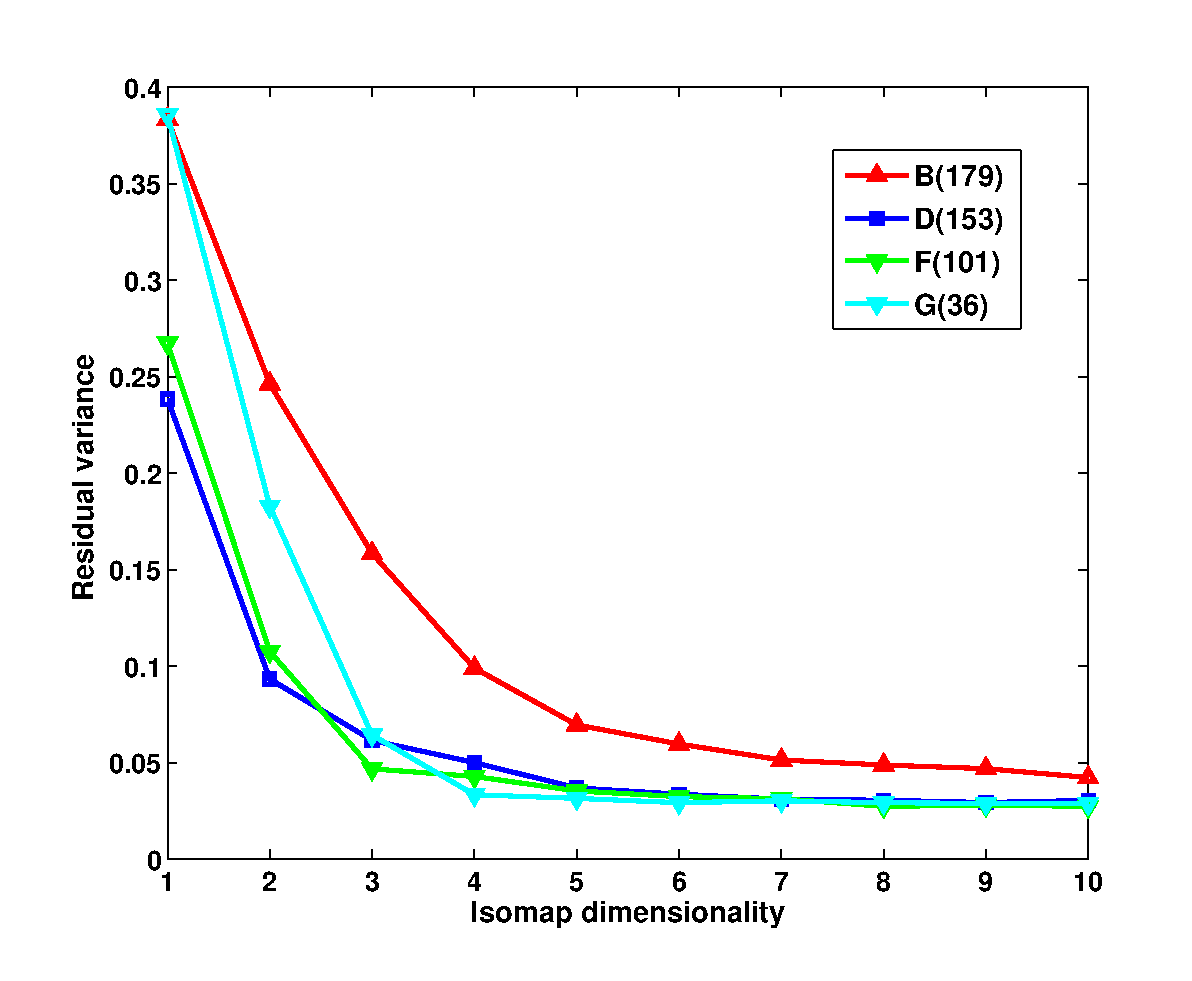
\includegraphics[width=62mm, height=52mm]{dia/gtvcrv2.eps}}
\caption{Isomap residual variances for clusters for the variable gear teeth
  problem. Residual variances for the clusters are similar to the whole
  pareto-front}
 \label{gtvClustersRV}
\end{center}\end{figure}

Cluster \textbf{A} has the largest number of optimal designs and occupies
the middle portion of the power range. Cluster \textbf{B} has the highest
power gearbox designs. \textbf{C} occupies the region between \textbf{A}
and \textbf{B}. All other clusters have low power gearbox designs with
\textbf{G} being the smallest and with the least power rating designs.
Having maximum output speed error as an objective doesn't provide any
additional useful choices to the designer, as this objective doesn't have
any trade-off or conflict with the other two objectives, turning this
optimization into essentially a two objective optimization.



The Isomap residual variances of the clusters shown in figure
\ref{gtvClustersRV} shows the clusters have manifold dimensionality similar
to the whole Pareto-front. The manifold dimensionality of the clusters
maybe 1 or 2 for most of the clusters though there are no precise
indications of the exact number of dimensions. The {\em minimization of
  error objective} in this case is an example of an {\em ill behaved}
objective function as discussed in section \ref{cdc} with reference to the
chunk dimensionality conjecture, as it doesn't monotonically increase or
decrease with the $n_{p_i}$ and $n_{w_i}$ variables. Nevertheless, the
dimensionality of the clusters are still in accordance with the conjectures
claim. The explained variance plots (figure \ref{gtvClustersEV}) present a
picture similar to that of the Isomap residual variances. The plots show
the cumulative explained variance of the principal components of the
clusters. For all the clusters the cumulative explained variance goes above
95\% only after the sixth principal component and the first three principal
components have quite significant explained variances.




\begin{figure}[ht]\begin{center}
 \subfloat[Clusters \textbf{A}, \textbf{B}, \textbf{C} and \textbf{D}]{
 \label{gt11rv} 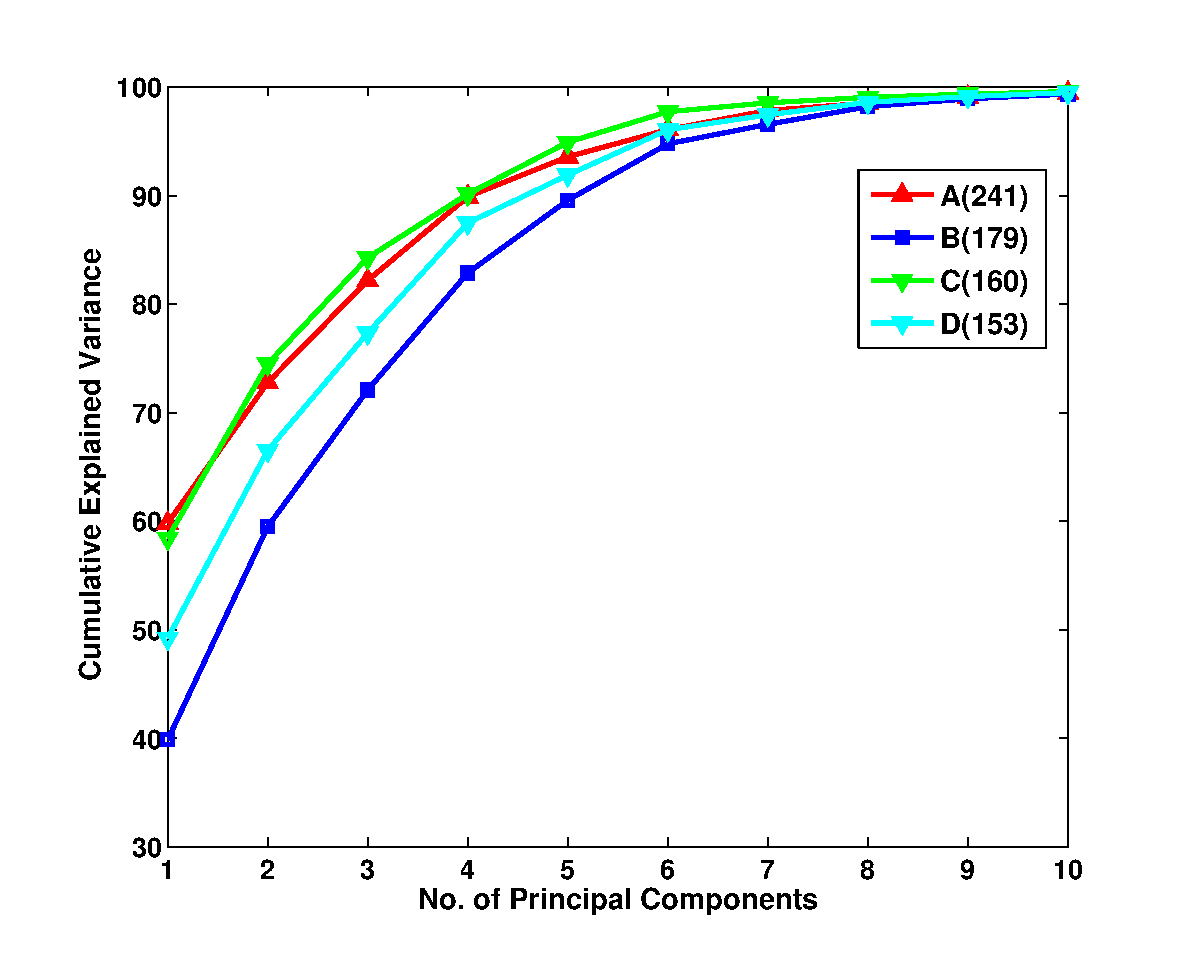
\includegraphics[width=62mm, height=52mm]{dia/gtvicev1.eps}}
 \subfloat[Clusters \textbf{E}, \textbf{F} and \textbf{G}]{
 \label{gt11ev} 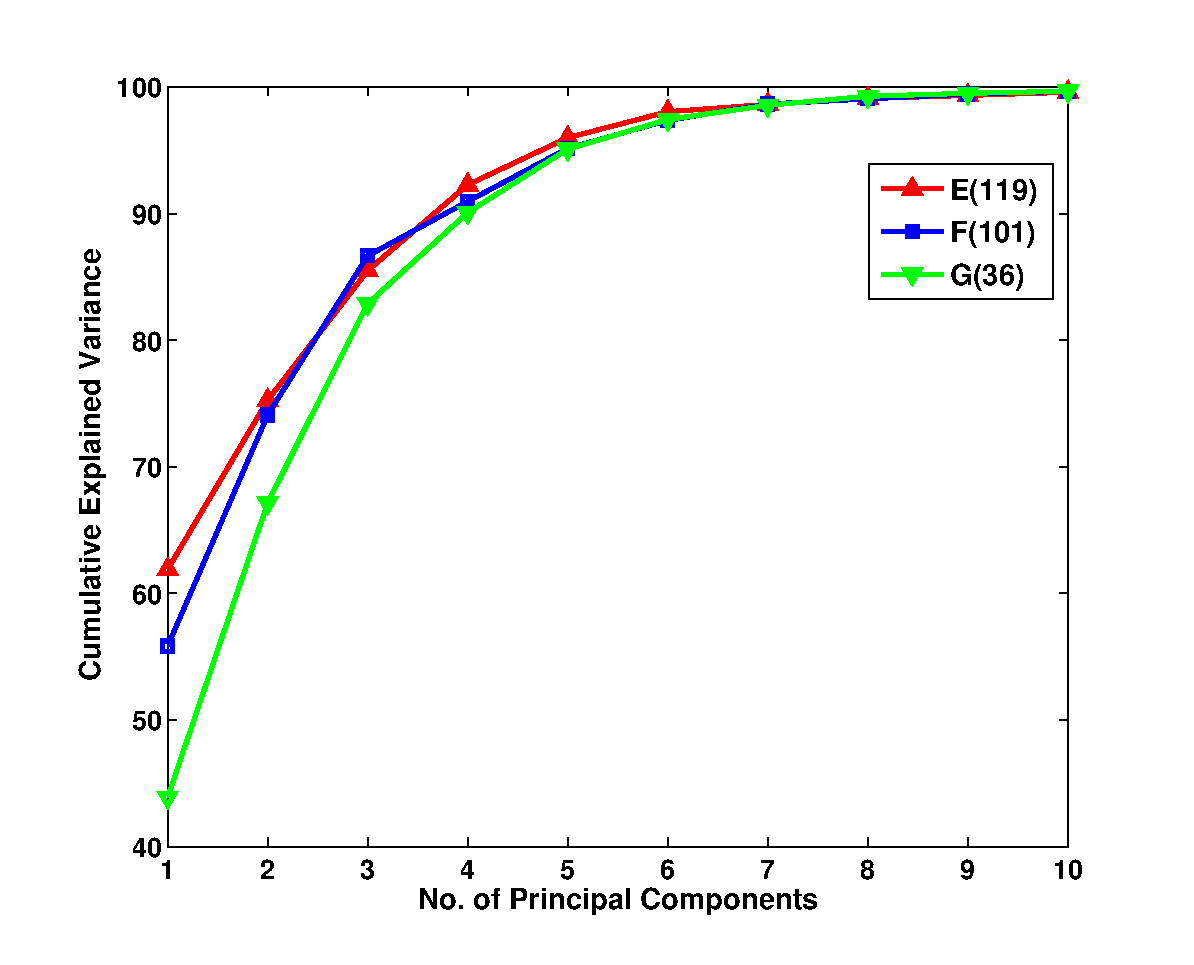
\includegraphics[width=62mm, height=52mm]{dia/gtvicev2.eps}}
 \caption{Cumulative PCA explained variance for 29 variable problem. For
  most clusters, first five-six principal components cover 90\% of the
  explained variance.}
 \label{gtvClustersEV}
\end{center}\end{figure}
 
In all the principal components number of teeth variables have the highest
weights. Unlike in the fixed layout gearbox design problem, power is not the 
dominant variable in the principal components. The $t_i$ variables have
weights lower than most of the number of the $n_i$ variables, except 
$n_{15}$, $n_{16}$, $n_{17}$ and $n_{18}$. Module is among the least important 
variables in all the principal components.

We have already explored the significance of the thickness variables and
module thickness in the pareto-front in the previous section. For this
reason, we will concentrate on the parts that the $n_i$ variables play in
the pareto-front clusters.  Table \ref{first2gtvnt} lists the $n_i$
variables in the sorted order of their absolute weights in the principal
components. The cells are shaded according to the transmission stage the
variable belongs to. The number of teeth variables of the second
transmission stage ($n_7$ to $n_{12}$) show the most amount of variability
while the last transmission stage has the most stable configuration showing
the least amount of variation in all the clusters.





   
{\tiny 

  \begin{table}[!ht]
    \centering
    \begin{tabular}{|c|c|c|c|c|c|c|c|c|c|c|c|c|}
      \hline
      \multirow{2}{*}{A} & First PC & \cellcolor[gray]{0.7} $n_{8}$ & \cellcolor[gray]{0.7} $n_{9}$ & \cellcolor[gray]{0.7} $n_{12}$ & \cellcolor[gray]{0.6} $n_{6}$ & \cellcolor[gray]{0.7} $n_{7}$ & \cellcolor[gray]{0.7} $n_{11}$ & $\dots$ & \cellcolor[gray]{0.9} $ n_{16}$ & \cellcolor[gray]{0.9} $n_{18}$ & \cellcolor[gray]{0.9} $n_{15}$ & \cellcolor[gray]{0.9} $n_{17}$ \\ \cline{2-13}
      & Second PC & \cellcolor[gray]{0.7} $n_{11}$ & \cellcolor[gray]{0.8} $n_{13}$ & \cellcolor[gray]{0.7} $n_{10}$ & \cellcolor[gray]{0.7} $n_{12}$ & \cellcolor[gray]{0.6} $n_{5}$ & \cellcolor[gray]{0.6} $n_{6}$ & $\dots$ & \cellcolor[gray]{0.9}  $n_{17}$ & \cellcolor[gray]{0.9}  $n_{16}$ & \cellcolor[gray]{0.9}  $n_{15}$ & \cellcolor[gray]{0.9} $n_{18}$ \\
      \hline
      \cline{1-13}
      \multirow{2}{*}{B}& First PC & \cellcolor[gray]{0.7} $n_{12}$ & \cellcolor[gray]{0.7} $n_{8}$ & \cellcolor[gray]{0.7} $n_{11}$ & \cellcolor[gray]{0.6} $n_{6}$ & \cellcolor[gray]{0.6} $n_{5}$ & \cellcolor[gray]{0.7} $n_{9}$ & $\dots$ & \cellcolor[gray]{0.9}  $n_{17}$ & \cellcolor[gray]{0.9}  $n_{15}$ & \cellcolor[gray]{0.9}  $n_{16}$ & \cellcolor[gray]{0.9} $n_{18}$ \\ 
      \cline{2-13}
      & Second PC & \cellcolor[gray]{0.7} $n_{11}$ & \cellcolor[gray]{0.7} $n_{10}$ & \cellcolor[gray]{0.7} $n_{8}$ & \cellcolor[gray]{0.7} $n_{12}$ & \cellcolor[gray]{0.6} $n_{6}$ & \cellcolor[gray]{0.8} $n_{13}$ & $\dots$ &  \cellcolor[gray]{0.9} $n_{15}$ & \cellcolor[gray]{0.9}  $n_{17}$ & \cellcolor[gray]{0.9} $n_{16}$ & \cellcolor[gray]{0.9} $n_{18}$ \\ 
      \hline
      \cline{1-13}
      \multirow{2}{*}{C}& First PC & \cellcolor[gray]{0.7} $n_{11}$ & \cellcolor[gray]{0.7} $n_{7}$ & \cellcolor[gray]{0.7} $n_{10}$ & \cellcolor[gray]{0.6} $n_{6}$ & \cellcolor[gray]{0.7} $n_{9}$ & \cellcolor[gray]{0.6} $n_{5}$ & $\dots$ &  \cellcolor[gray]{0.9}  $n_{17}$ & \cellcolor[gray]{0.9} $n_{18}$ & \cellcolor[gray]{0.9} $n_{15}$ & \cellcolor[gray]{0.9} $n_{16}$ \\ 
      \cline{2-13}
      & Second PC & \cellcolor[gray]{0.7} $n_{12}$ & \cellcolor[gray]{0.6} $n_{6}$ & \cellcolor[gray]{0.7} $n_{8}$ & \cellcolor[gray]{0.7} $n_{11}$ & \cellcolor[gray]{0.7} $n_{9}$ & \cellcolor[gray]{0.7} $n_{10}$ & $\dots$ &  \cellcolor[gray]{0.9}  $n_{15}$ & \cellcolor[gray]{0.9} $n_{16}$ & \cellcolor[gray]{0.9} $n_{18}$ & \cellcolor[gray]{0.9} $n_{17}$ \\ 
      \hline
      \cline{1-13}
      \multirow{2}{*}{D}& First PC & \cellcolor[gray]{0.7} $n_{9}$ & \cellcolor[gray]{0.7} $n_{8}$ & \cellcolor[gray]{0.7} $n_{10}$ & \cellcolor[gray]{0.6} $n_{5}$ & \cellcolor[gray]{0.7} $n_{12}$ & \cellcolor[gray]{0.7} $n_{7}$ & $\dots$ &  \cellcolor[gray]{0.9}  $n_{15}$ & \cellcolor[gray]{0.9} $n_{16}$ & \cellcolor[gray]{0.9} $n_{17}$ & \cellcolor[gray]{0.9}  $n_{18}$ \\ 
      \cline{2-13}
      & Second PC & \cellcolor[gray]{0.7} $n_{10}$ & \cellcolor[gray]{0.7} $n_{12}$ & \cellcolor[gray]{0.7} $n_{11}$ & \cellcolor[gray]{0.7} $n_{7}$ & \cellcolor[gray]{0.6} $n_{6}$ & \cellcolor[gray]{0.7} $n_{8}$ & $\dots$ &  \cellcolor[gray]{0.9} $n_{17}$ & \cellcolor[gray]{0.9} $n_{15}$ & \cellcolor[gray]{0.9} $n_{18}$ & \cellcolor[gray]{0.9}  $n_{16}$ \\ 
      \hline
      \cline{1-13}
      \multirow{2}{*}{E}& First PC & \cellcolor[gray]{0.7} $n_{8}$ & \cellcolor[gray]{0.7} $n_{9}$ & \cellcolor[gray]{0.7} $n_{12}$ & \cellcolor[gray]{0.6} $n_{6}$ & \cellcolor[gray]{0.7} $n_{11}$ & \cellcolor[gray]{0.8} $n_{13}$ & $\dots$ &  \cellcolor[gray]{0.9} $n_{18}$ & \cellcolor[gray]{0.9} $n_{17}$ & \cellcolor[gray]{0.9} $n_{15}$ & \cellcolor[gray]{0.9}  $n_{16}$ \\ 
      \cline{2-13}
      & Second PC & \cellcolor[gray]{0.7} $n_{9}$ & \cellcolor[gray]{0.7} $n_{8}$ & \cellcolor[gray]{0.7} $n_{12}$ & \cellcolor[gray]{0.7} $n_{7}$ & \cellcolor[gray]{0.7} $n_{10}$ & \cellcolor[gray]{0.6} $n_{4}$ & $\dots$ &  \cellcolor[gray]{0.9} $n_{16}$ & \cellcolor[gray]{0.9} $n_{15}$ & \cellcolor[gray]{0.9} $n_{17}$ & \cellcolor[gray]{0.9} $n_{18}$ \\ 
      \hline
      \cline{1-13}
      \multirow{2}{*}{F}& First PC & \cellcolor[gray]{0.7} $n_{11}$ & \cellcolor[gray]{0.7} $n_{9}$ & \cellcolor[gray]{0.6} $n_{6}$ & \cellcolor[gray]{0.7} $n_{8}$ & \cellcolor[gray]{0.6} $n_{5}$ & \cellcolor[gray]{0.7} $n_{7}$ & $\dots$ &  \cellcolor[gray]{0.9}  $n_{16}$ & \cellcolor[gray]{0.9}  $n_{15}$ & \cellcolor[gray]{0.9} $n_{18}$ & \cellcolor[gray]{0.9} $n_{17}$ \\ 
      \cline{2-13}
      & Second PC & \cellcolor[gray]{0.7} $n_{8}$ & \cellcolor[gray]{0.6} $n_{6}$ & \cellcolor[gray]{0.7} $n_{7}$ & \cellcolor[gray]{0.7} $n_{9}$ & \cellcolor[gray]{0.7} $n_{11}$ & \cellcolor[gray]{0.6} $n_{5}$ & $\dots$ &  \cellcolor[gray]{0.9} $n_{16}$ & \cellcolor[gray]{0.9} $n_{18}$ & \cellcolor[gray]{0.9} $n_{17}$ & \cellcolor[gray]{0.9} $n_{15}$ \\ 
      \hline
      \cline{1-13}
      \multirow{2}{*}{G}& First PC & \cellcolor[gray]{0.7} $n_{11}$ & \cellcolor[gray]{0.8} $n_{13}$ & \cellcolor[gray]{0.6} $n_{6}$ & \cellcolor[gray]{0.7} $n_{7}$ & \cellcolor[gray]{0.7} $n_{9}$ & \cellcolor[gray]{0.7} $n_{8}$ & $\dots$ &  \cellcolor[gray]{0.9} $n_{17}$ & \cellcolor[gray]{0.9} $n_{15}$ & \cellcolor[gray]{0.9} $n_{16}$ & \cellcolor[gray]{0.9}  $n_{18}$ \\ 
      \cline{2-13}
      & Second PC & \cellcolor[gray]{0.7} $n_{12}$ & \cellcolor[gray]{0.6} $n_{4}$ & \cellcolor[gray]{0.7} $n_{8}$ & \cellcolor[gray]{0.7} $n_{10}$ & \cellcolor[gray]{0.7} $n_{9}$ & \cellcolor[gray]{0.7} $n_{11}$ & $\dots$ &  \cellcolor[gray]{0.9}  $n_{17}$ & \cellcolor[gray]{0.9}  $n_{16}$ & \cellcolor[gray]{0.9} $n_{15}$ & \cellcolor[gray]{0.9} $n_{18}$ \\ 
      \hline
    \end{tabular}
    \caption{Ranking of gear teeth variables on the basis of absolute weights in principal components. The gear pairs of the last transmission stage occupy the last positions indicating they are the least varying.}
    \label{first2gtvnt}
  \end{table}
}


\subsection{Discussion}
Although power is still an objective in the multi-objective optimization,
 since there are three objectives (\emph{volume} and \emph{maximum error
  in output speeds} being the other two), a number of designs with same
power rating are possible, hence power is not a dominant variable in the
principal components. As observed earlier, having error as a third
objective isn't useful in the design process, as having higher error
apparently neither reduces the volume significantly nor improves the power
characteristics of the designs. 


\begin{figure}[ht]\begin{center}
 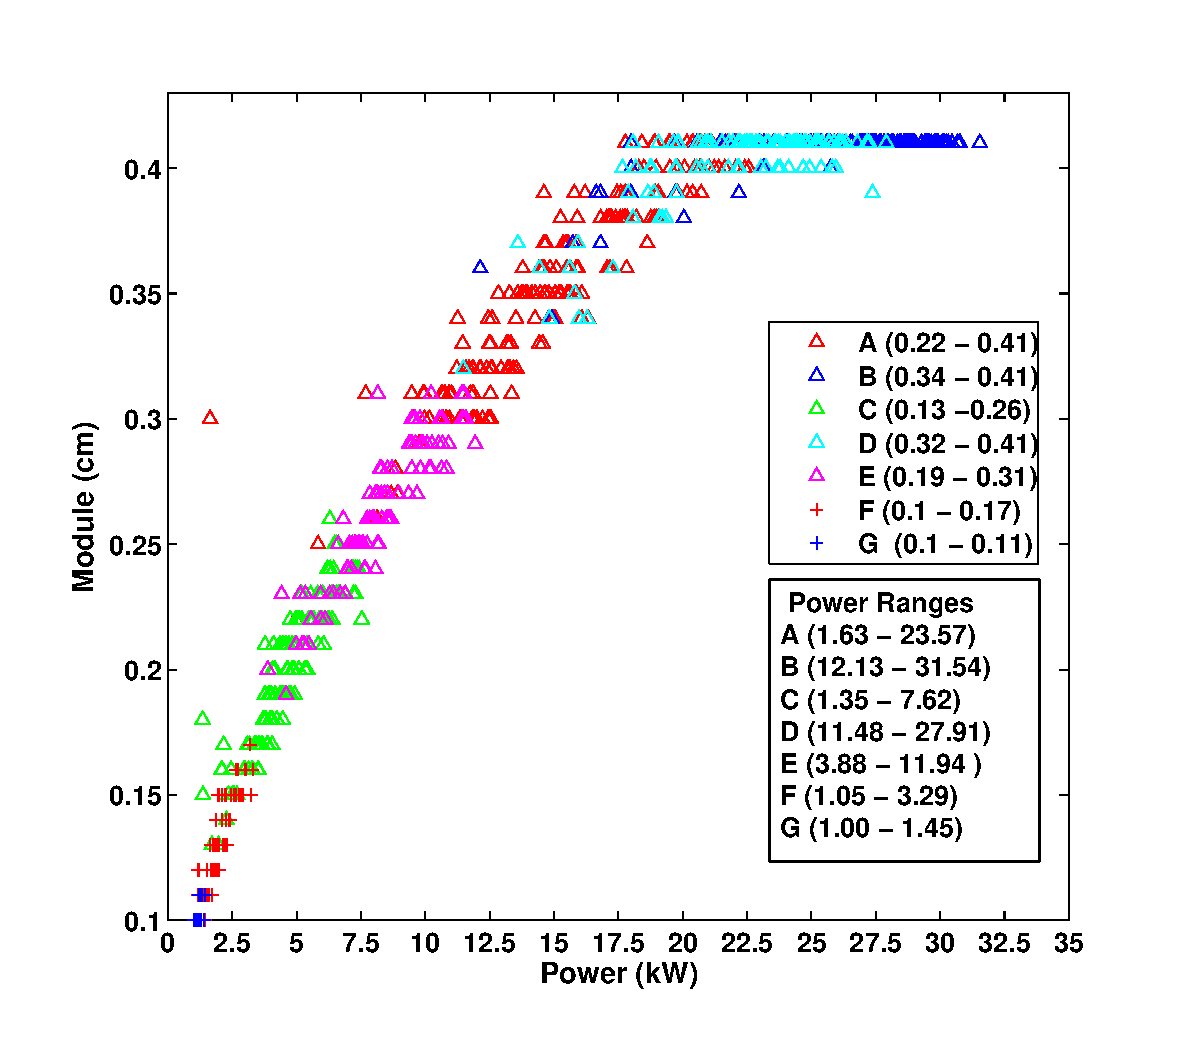
\includegraphics[width=100mm, height=80mm]{dia/gtvpVsm.eps}
 \caption{Power Vs. module characteristics of the pareto-front for 29
   variable problem. Clusters show intermingling unlike for the fixed layout
   problem.}
 \label{gtvpVsm}
\end{center}\end{figure}

The final transmission stage has to withstand the highest stresses, so the
module choice for the gear-box has to be able to withstand the stresses in
the final transmission stage. The same module is used in the gears of all
the transmission stages.  The number of teeth has to be kept minimum
possible as it also affects gearbox volume directly. Also there is a limit
on the maximum transmission ratio. All these trade-offs and limitations
lead to limited choices for the number of teeth variables in the final
transmission stage. On the other hand, in the second transmission stage
($n_{7}$ - $n_{12}$) has to withstand smaller stresses than the last stage,
it can meet the same stress requirements by increasing the number of teeth
and decreasing the gear pair thicknesses while maintaining the required
transmission ratios. This explains the positions of the number of teeth
variables in the last and second transmission stage.


The module to power characteristics are similar to the fixed layout case,
as shown in figure \ref{gtvpVsm}. Unlike in the previous case, designs
in different clusters can have the same module width. 


% \multirow{2}{*}{}& First PC & $n_{}$ & $n_{}$ & $n_{}$ & $n_{}$ & $n_{}$ & $n_{}$ & $\dots$ &  \cellcolor{} $n_{}$ & \cellcolor{} $n_{}$ & \cellcolor{}$n_{}$ & \cellcolor{} $n_{}$ \\ 
%\cline{2-13}
% & Second PC & $n_{}$ & $n_{}$ & $n_{}$ & $n_{}$ & $n_{}$ & $n_{}$ & $\dots$ &  \cellcolor{} $n_{}$ & \cellcolor{} $n_{}$ & \cellcolor{}$n_{}$ & \cellcolor{} $n_{}$ \\ 
%\hline


\chapter{More Design Problems}
In this chapter we present the results of our chunking and analysis
methodology on two problems. The first problem is the multiple disk clutch
brake design problem, a discreet optimization problem with five variables
and two objectives. The other is the welded beam design problem which is
continuous decision space problem with four variables and two objectives.

\section{Problem Introduction}
\subsection{Multiple-disk clutch brake design problem}


\begin{figure}[ht]\begin{center}
 \fbox{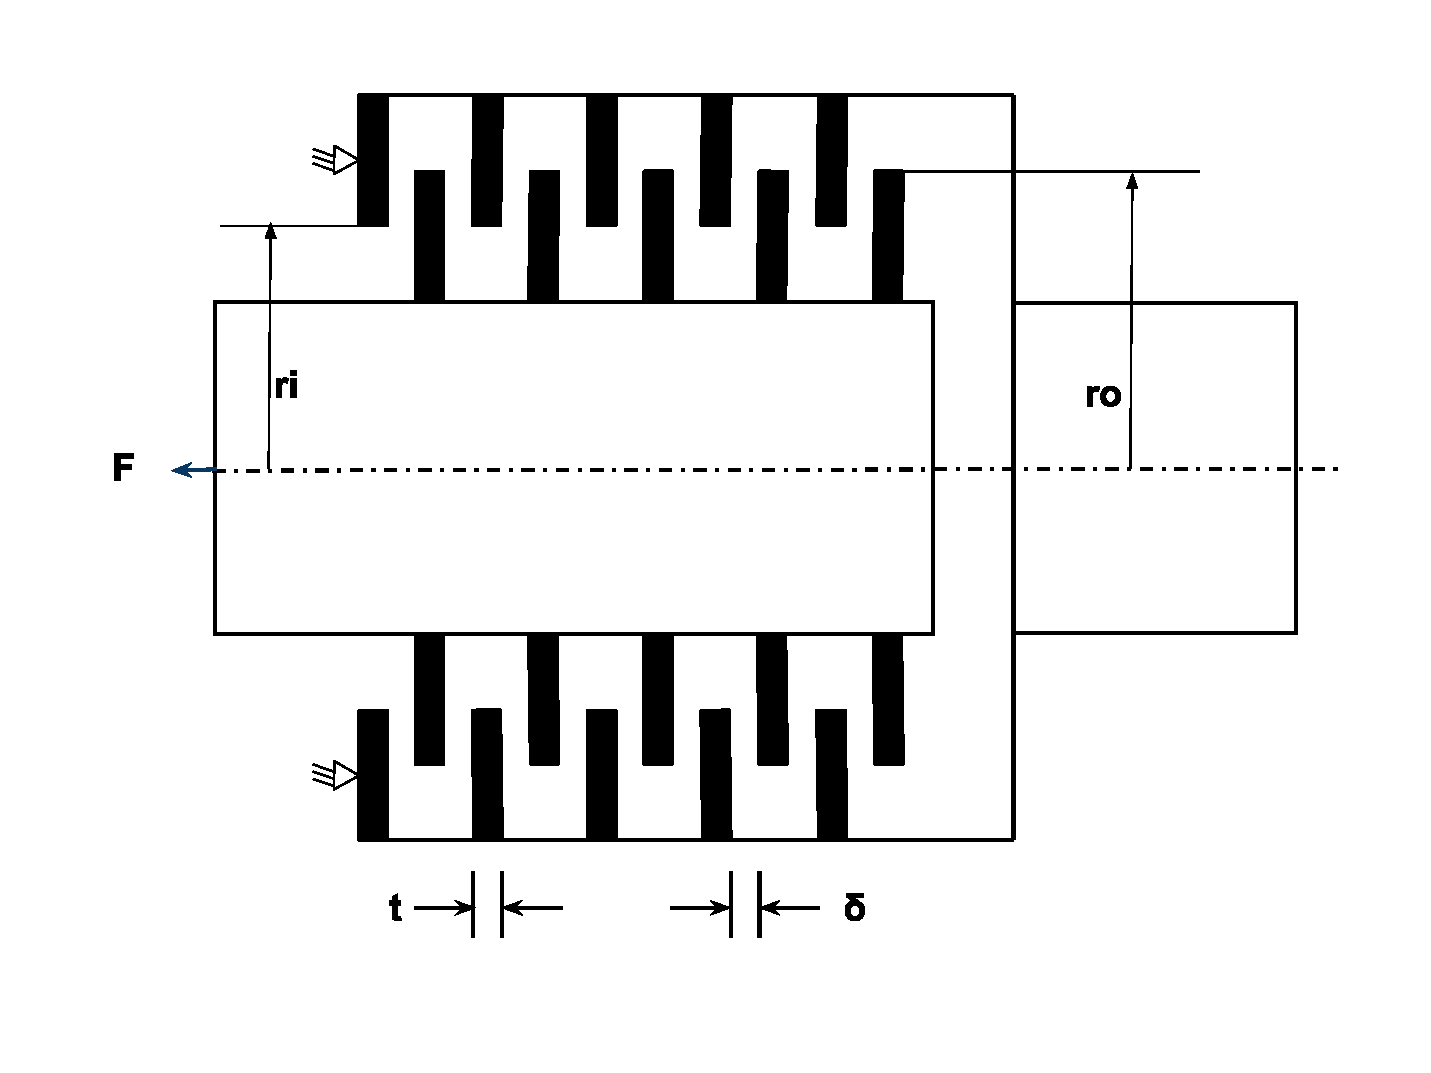
\includegraphics[width=75mm, height=60mm]{dia/clutchbrake.eps}}
 \caption{Schematics of a multiple disk clutch brake.}
 \label{clutchbrake}
\end{center}\end{figure}


We have adopted the problem specification used in \citep{deb06}. The
schematics of a multiple-disk clutch brake are shown in figure
\ref{clutchbrake}. Two conflicting objectives are considered in this 
optimization problem:
{\allowdisplaybreaks \begin{enumerate}
  \item minimization of mass, and,
  \item minimization of stopping time.
\end{enumerate}
This optimization problem is defined on five decision variables $\vec{x} = (r_i, r_o, t, F, Z)$, where:
\begin{enumerate}
  \item $r_i \in [60, 80]$ (in steps of one) is the inner radius in mm,
  \item $r_o \in [91, 110]$ (in steps of one) is the outer radius in mm,
  \item $t \in [1, 3]$ (in steps of 0.5) is the thickness of disks in mm,
  \item $F \in [600, 1000]$ (in steps of 10) is the actuating force in N and
  \item $Z \in [2, 10]$ (in steps of one) is the number of friction
    surfaces or disks.
\end{enumerate}}

The complete optimization problem is formulated as follows:

\begin{singlespacing}
\begin{flushleft}

{\allowdisplaybreaks
  \begin{align}
    \text{Maximize} \quad & f_1(\vec{x}) =  \pi (x_{2}^{2} - x_{1}^{2}) x_3 (x_5  + 1) \rho,\\
    \text{Minimize} \quad & f_2(\vec{x}) = T = \left. \frac{I_{z} \omega} {M_{h} + M_{f}} \right.,\\
    \text{Subject to,} & \nonumber \\
    \qquad &g1(\vec{x}) =  \left. x_2 - x_1 - \Delta R \geqslant 0 \right.,\\
    \qquad &g2(\vec{x}) = \left. L_{max} - (x_5 + 1)(x_3 + \delta) \geqslant 0 \right. \\
    \qquad &g3(\vec{x}) = \left. p_{max} - p_{rz} \geqslant 0 \right.\\
    \qquad &g4(\vec{x}) = \left. p_{max} V_{sr,max} - p_{rz} V_{sr} \geqslant 0 \right., \\
    \qquad &g5(\vec{x}) = \left. V_{sr, max} - V_{sr} \geqslant 0 \right., \\
    \qquad &g6(\vec{x}) = \left. M_{h} - s M_{s} \geqslant 0 \right., \\
    \qquad &g7(\vec{x}) = \left. T \geqslant 0 \right., \\
    \qquad &g8(\vec{x}) = \left. T_{max} - T \geqslant 0 \right.
  \end{align}
}

Where, 

\begin{itemize}
  \item $ M_h = \dfrac{2}{3} \mu x_4 x_5 \dfrac{x_{2}^3 - x_{1}^3}{x_2^2 - x_{1}^2} $ N.mm,
  \item $ \omega = \dfrac {\pi n}{30} $ rad/s ,
  \item $ A = \pi(x_2^2 - x_1^2) \quad \text{mm}^2$ ,
  \item $ p_{rz} = \dfrac{x_{4}}{A} \quad \text{N/mm}^2$,
  \item $ V_{sr} = \dfrac{\pi R_{sr} n} {30} $ mm/s ,
  \item $ R_{sr} = \dfrac{2}{3} \dfrac{x_{2}^3 - x_{1}^3}{x_2^2 - x_1^2} $ mm ,
  \item $ \Delta R = 20 $ mm ,
  \item $ L_{max} = 30 $ mm ,
  \item $ \mu = 0.5$ ,
  \item $p_{max} = 1 \quad \text{MPa}$, 
  \item $\rho = 0.0000078 \text{kg/mm}^3$,
  \item $V_{sr,max} = 10 \quad \text{m/s}$,
  \item $s = 1.5$,
  \item $T_{max} = 15 \quad \text{s}$, 
  \item $n = 250 \quad \text{rpm}$,
  \item $M_s = 40 \quad \text{Nm}$,
  \item $M_f = 3 \quad \text{Nm}$,
  \item $I_z = 55 \quad \text{kg.m}^2$,
  \item $\delta = 0.5 \quad \text{mm}$,
\end{itemize}

\end{flushleft}

\end{singlespacing}
    

\subsection{The welded beam design problem}



\begin{figure}[ht]\begin{center}
 \fbox{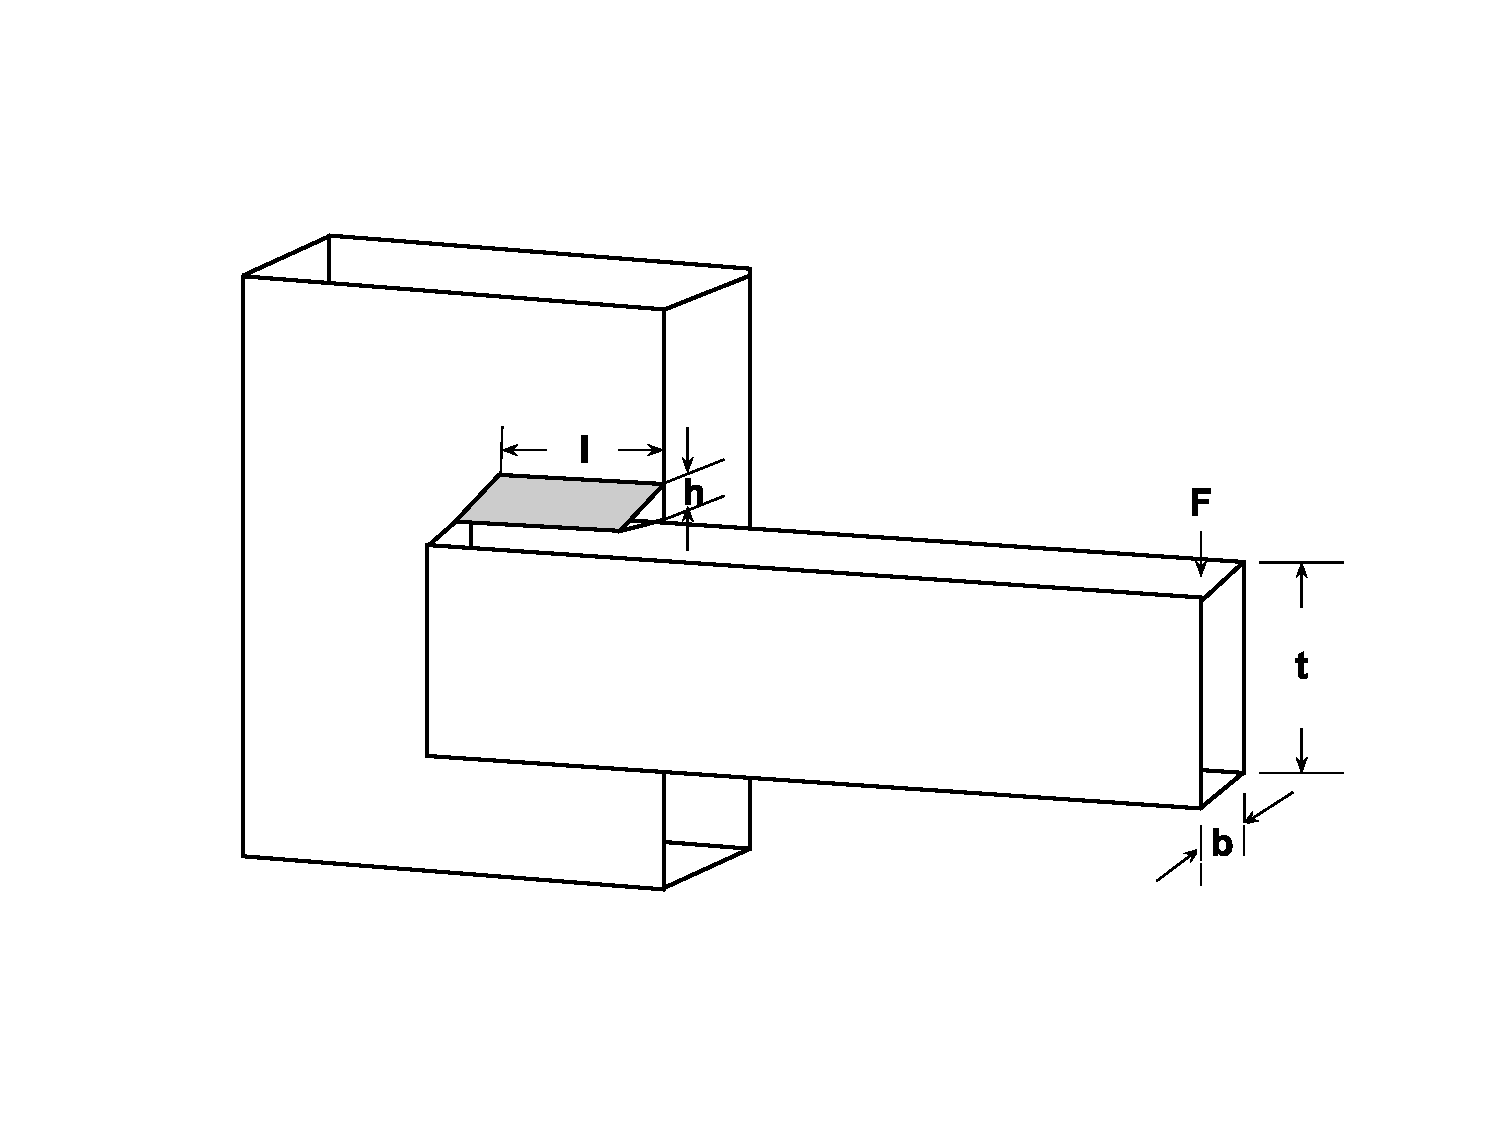
\includegraphics[width=75mm, height=60mm]{dia/wbeam.eps}}
 \caption{Schematics of a welded beam.}
 \label{wbeam}
\end{center}\end{figure}


Welded beam design problem is a well known Multi-objective optimization
problem. Here we adopt the formulation given in \citep{deb10}. The
objective of this problem is to minimize the cost and end deflection of a
beam welded at one end and supporting a load $ F = 6000$ lb at the other.
The overhang portion of the beam has a length of 14 in.There are four
design variables:
\begin{enumerate}
  \item $b \in [0.125, 5] $ thickness of the beam,
  \item $t \in [0.1, 10] $ width of the beam,
  \item $l \in [0.1, 10] $ length of the weld and
  \item $h \in [0.125, 5] $ thickness of the weld.
\end{enumerate}

The complete multi-objective formulation is as follows:

\begin{singlespacing}
  \begin{align}
    \text{Minimize} \quad &f_1(\vec{x}) = C = \left. 1.1047 h ^2 l + 0.04811 t b(14.0 + l) \right. \\
    \text{Minimize} \quad &f_2(\vec{x}) = D = \left. \dfrac{2.1952}{t^3 b} \right. \\
  \text{Subject to:}  & \nonumber \\
  \qquad &g_1(\vec{x}) = \left. 13600 - \tau (\vec{x}) \geqslant 0 \right. ,\\
  \qquad &g_2(\vec{x}) = \left. 30000 - \sigma (\vec{x}) \geqslant 0 \right.,\\
  \qquad &g_3(\vec{x}) = \left. b - h \geqslant 0 \right., \\
  \qquad &g_4(\vec{x}) = \left. P_c(\vec{x}) - 6000 \geqslant 0 \right. 
\end{align}

% \begin{align}
% \end{align}

Where,

\begin{itemize}
  \item $ \tau (\vec{x}) = \sqrt{ \dfrac{(\tau ')^2 + (\tau'')^2 + (l \tau' \tau'')} {\sqrt{ 0.25(l^2 + (h + t)^2)}}}$,
  \item $ \tau' = \dfrac {6000} {\sqrt{2} h l}$,
  \item $ \tau'' = \dfrac { 6000 (14 + 0.5l) \sqrt{0.25(l^2 + (h + t) ^2 )}} { 2 [0.707 h l (\frac{l^2}{12} + 0.25 (h + t) ^2)] } $,
  \item $ \sigma (\vec{x}) = \dfrac {504000} {t^2 b} $,
  \item $P_c (\vec{x}) = 64746.022(1-0.0282346t) t b^3$.
\end{itemize}

\end{singlespacing}    

\section{Analysis of the clutch brake design problem}

Figure \ref{clutch} shows the pareto-front obtained after running local
search on NSGA-II output. NSGA-II was run for 300 generations with a
population size of 5000 and yielded 125 near optimal solutions. The
probability for crossover and mutation were set to 0.79 and 0.5
respectively. Running local search gives a pareto-front consisting of 95
optimal solutions.

\begin{figure}[ht]\begin{center}
 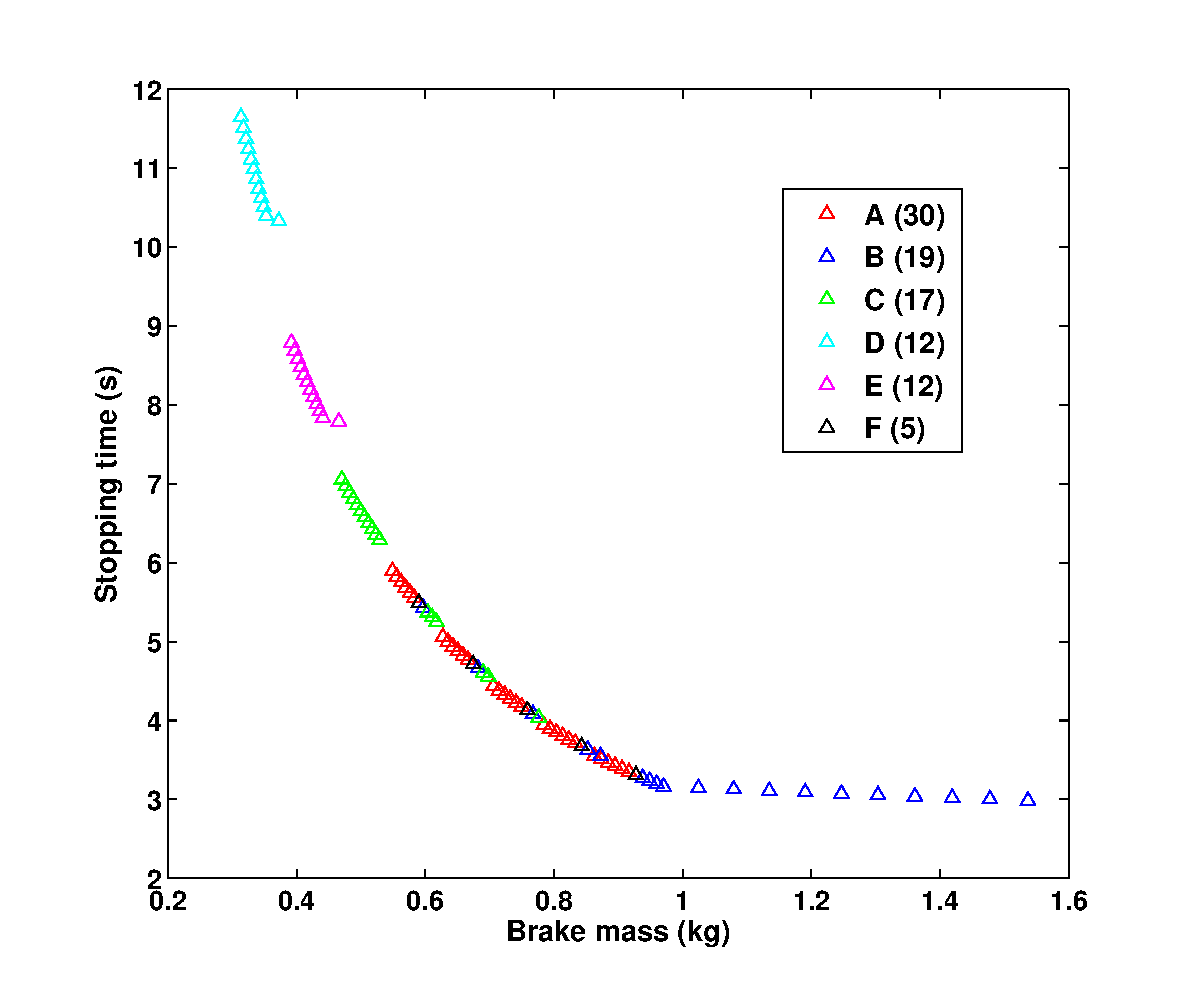
\includegraphics[width=100mm, height=80mm]{dia/clutchParetoClusters.eps}
 \caption{Pareto-front and the clusters of the multiple-disk clutch brake
   design problem. Clusters obtained with $k = 1.9$}
 \label{clutch}
\end{center}\end{figure}


\subsection{Isomap and PCA analysis of the pareto-front} 
Figure \ref{clutchwrv} and \ref{clutchwev} show the results of running
Isomap and PCA on the pareto-front of the clutch brake design problem. The
drop in the residual variance curve for the second Isomap dimension
indicates a manifold dimensionality of one. The PCA explained variance,
however, shows two principal components with significant explained
variances, the first with 80\% explained variance and the second with 17\%.


\begin{figure}[ht]\begin{center}
 \subfloat[Isomap Residual Variance.]{
 \label{clutchwrv} 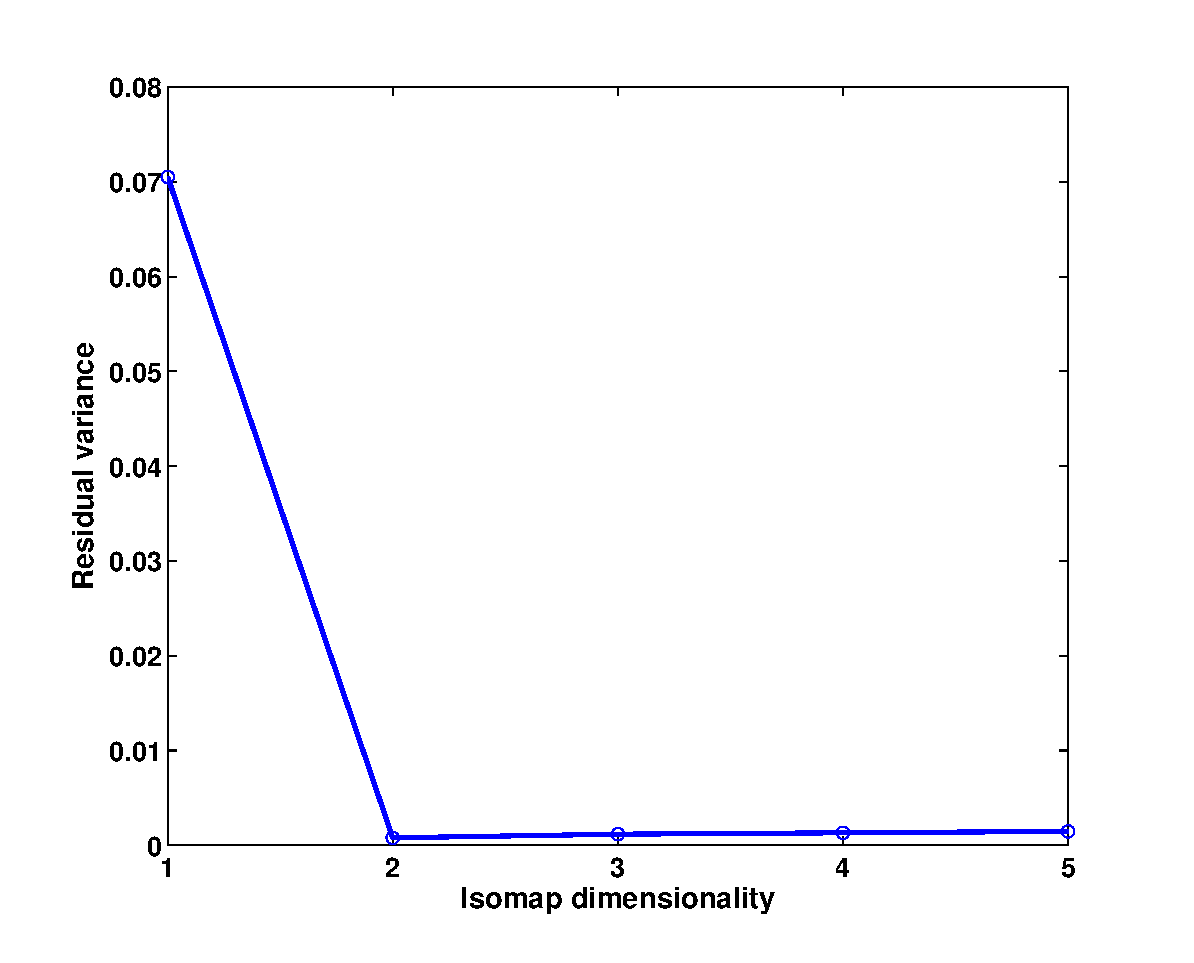
\includegraphics[width=62mm, height=52mm]{dia/clutchRV.eps}}
 \subfloat[PCA Explained variance.]{
 \label{clutchwev} 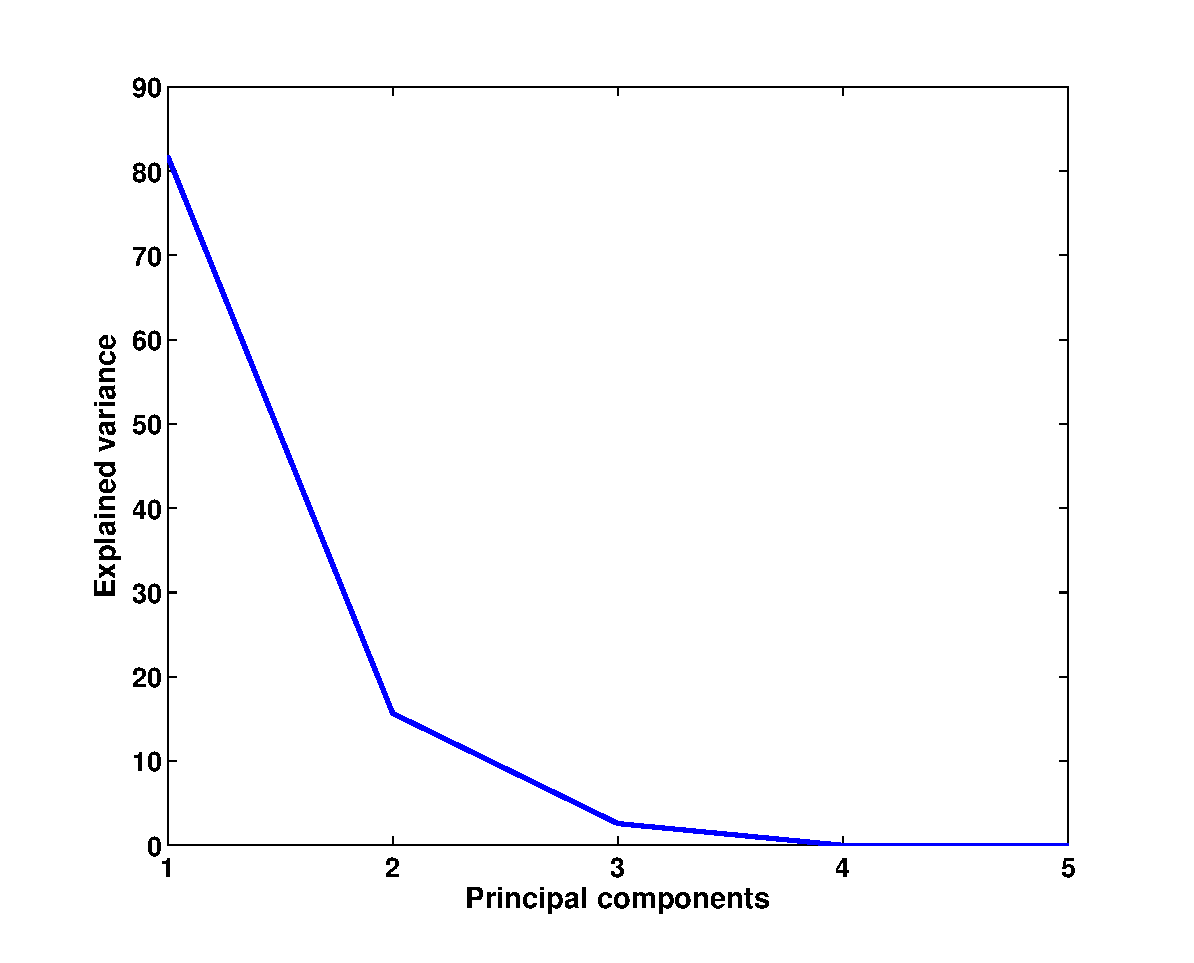
\includegraphics[width=62mm, height=52mm]{dia/clutchEV.eps}}
\caption{Isomap and PCA results for the pareto-front of multiple-disk
  clutch brake problem pareto-front. The manifold dimensionality is one as
  indicated in the Isomap residual variance plot but the PCA explained
  variance shows two significant principal components.}
 \label{clutchWholeVar}
\end{center}\end{figure}

Table \ref{first2clutchPCs} shows the first two significant components of
the pareto-front. Outer radius ($r_o$) has the highest weight in the
first principal component followed by inner radius ($r_i$). The number of
surfaces also has some variation. In the second principal component number
of surfaces ($Z$) is the dominant variable followed by inner radius with a
small weight. The variables thickness ($t$) and actuating force ($F$)
have zero weights in both the significant principal components indicating
they have the same values for all the optimal solutions. The thickness and
actuating force are fixed at the minimum and maximum possible values of 1
and 1000 respectively for all the optimal solutions.


\begin{table}[!ht]
  \centering
  \begin{tabular}{c|c|c|c|c|c|}
    \cline{2-6}
    & $r_{i}$ & $r_{o}$ & $ t $  & $F$ & $Z$ \\
    \hline
    \multicolumn{1}{|c|}{First PC} & 0.578 & 0.806 & 0 & 0 & 0.119\\
    \hline
    \multicolumn{1}{|c|}{Second PC} & -0.207 & 0.004 & 0 & 0 & 0.978\\
    \hline
  \end{tabular}
  \caption{First two principal components of the clutch brake design problem pareto-fron}
  \label{first2clutchPCs}
\end{table}

\subsection{Clustering analysis}
The pareto-front of this problem has a small number (95) of optimal
solutions. The $k$ parameter of the clustering algorithm had to be adjusted
accordingly to obtain a proper distribution of points in clusters. Six
clusters were obtained with $k = 1.9$. The clusters are shown in figure
\ref{clutch}.

Cluster \textbf{A} is the largest cluster with 37 points. It has the
mid-range designs of the clutch brake with stopping times ranging from 3.2
seconds to 6 seconds. Cluster \textbf{B} is composed of the heaviest and
most powerful brake designs, apart from some mid-range designs. It's the
only cluster having designs with weights in excess of 1 kg. Below 1 kg
designs follow a parabolic time vs. weight characteristics, but above 1 kg
designs show a linear relationship, an increase in weight yielding very
little benefit in stopping time. Clusters \textbf{D} and \textbf{E} have
the low end designs with stopping times in excess of 7.5 s. These are the
only clusters that appear as single contiguous chunks in the
pareto-front. Clusters \textbf{A}, \textbf{B}, \textbf{C} and \textbf{E}
have designs in overlapping objective ranges.

Isomap residual variances of the clusters (figure \ref{clutchcrv})
indicate one dimensional manifolds for the clusters, similar to the whole
pareto-front. This verifies the claims of the {\em chunk dimensionality
  conjecture} (section \ref{cdc}). Clusters \textbf{B-C} and \textbf{D-E}
have exactly same residual variances.  Cluster \textbf{A} has the highest
error in reverse mapping the one dimensional Isomap embedding. Clusters
\textbf{D} and \textbf{E} have negligible residual variances. PCA explained
variances for the clusters (figure \ref{clutchcev}) show a single
significant principal component for all the clusters except cluster
\textbf{A}.


\begin{figure}[ht]\begin{center}
 \subfloat[Isomap Residual Variance.]{
 \label{clutchcrv} 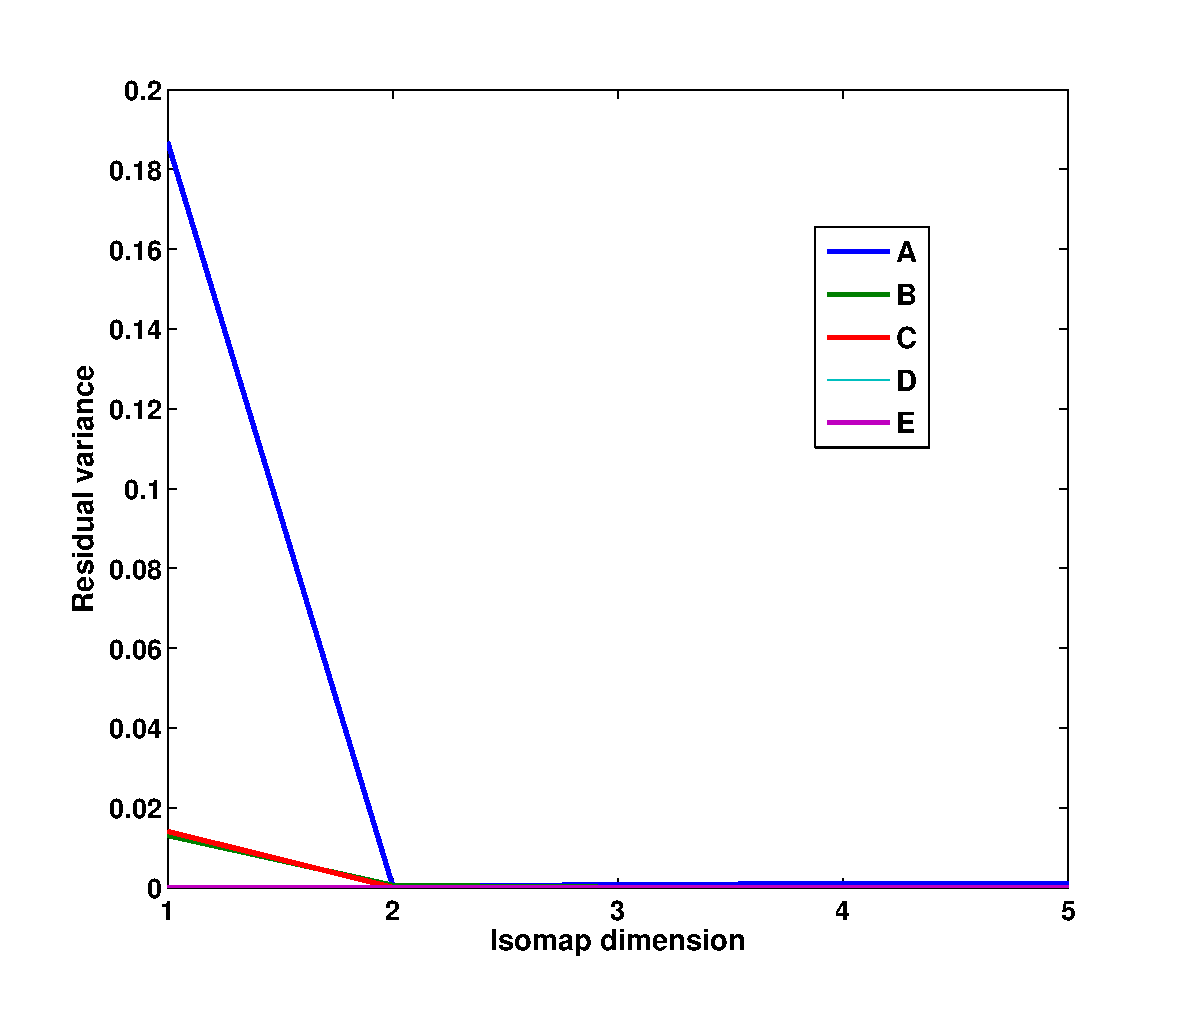
\includegraphics[width=62mm, height=52mm]{dia/clutchClustersRV.eps}}
 \subfloat[PCA Explained variance.]{
 \label{clutchcev} 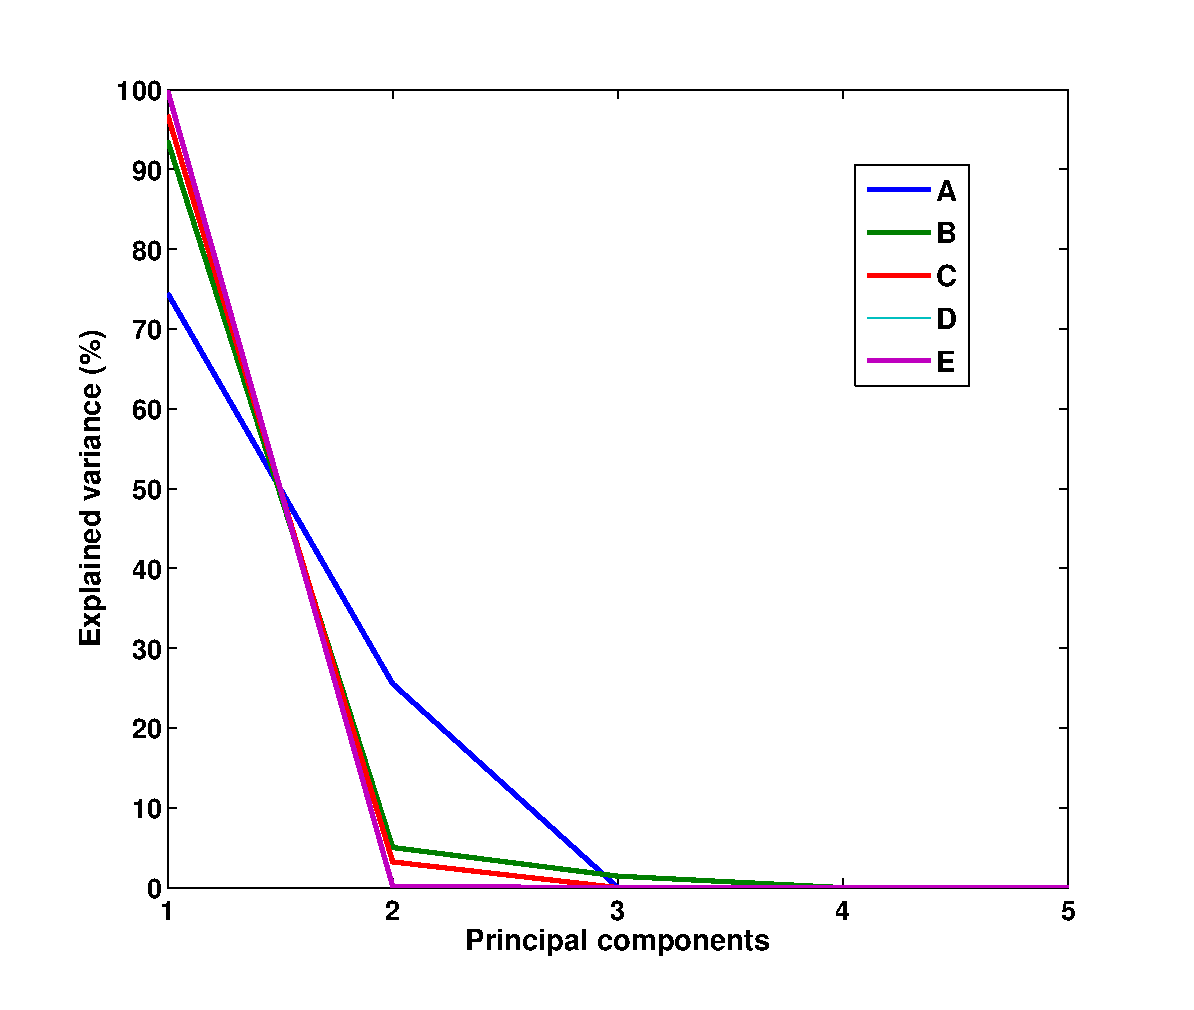
\includegraphics[width=62mm, height=52mm]{dia/clutchClustersEV.eps}}
\caption{Isomap and PCA results for the clusters of multiple-disk clutch
  brake problem. The manifold dimensionality of all the clusters is one,
  though cluster \textbf{A} has linear dimensionality of two indicated by
  two significant principal components in its explained variance plot.}
 \label{clutchClustersVar}
\end{center}\end{figure}


\begin{table}[!ht]
  \centering
  \begin{tabular}{c|c|c|c|c|c|}
    \cline{2-6}
    & $r_{i}$ & $r_{o}$ & $ t $  & $F$ & $Z$ \\
    \hline
    \multicolumn{1}{|c|}{\multirow{2}{*}{\textbf{A}}} & 0.707 & 0.707 & 0 & 0 & 0\\ \cline{2-6}
    \multicolumn{1}{|c|}{}& 0 & 0 & 0 & 0 & 1\\
    \hline
    \multicolumn{1}{|c|}{\textbf{B}} & 0.236 & 0.960 & 0 & 0 & 0.146\\
    \hline
    \multicolumn{1}{|c|}{\textbf{C}} & 0.703 & 0.703 & 0 & 0 & 0.097\\
    \hline
    \multicolumn{1}{|c|}{\textbf{D}} & 0.694 & 0.719 & 0 & 0 & 0\\
    \hline
    \multicolumn{1}{|c|}{\textbf{E}} & 0.694 & 0.719 & 0 & 0 & 0\\
    \hline
    \multicolumn{1}{|c|}{\textbf{F}} & 0 & 0 & 0 & 0 & 1\\
    \hline
  \end{tabular}
  \caption{Significant principal components of the clutch brake design problem clusters. $t$ and $F$ have no weights in any principal component. The inner and outer radii($r_i$ and $r_o$) show the highest variation for each cluster. The second component is parallel to the {\em number of friction surfaces (Z)} dimension.}
  \label{first2clutchPCs}
\end{table}

Table \ref{first2clutchPCs} shows the principal components of the
clusters. For most of the clusters, the radius variables have similar
weights. In cluster \textbf{B} the outer radius has higher weight than the
inner radius.  The second principal component of cluster \textbf{A} has
entirely composed of a single variable $Z$ only. Clusters \textbf{D} and
\textbf{E} have exactly the same components. The cluster \textbf{F} has 
variable $Z$ as its single Principal component.

\subsection{Discussion}

The most important fact that comes out of this analysis is that all optimal
clutch brakes should be designed with disks with smallest possible
thickness.  Secondly, a clutch brake must be designed for maximum actuating
force only, since the stopping time is inversely proportional to the
actuating force. The stopping time is also dependent on the friction area
as is evident from the figure \ref{clutchrVsZ}. A higher outer radius and a
larger number of friction surfaces (no. of disks) allow for a larger
contact area, but increasing the number of disks also increases the weight
of the design.  This trade-off is visible in all the clusters. The fact
that radius variables show greater variation across all clusters suggests
that to reduce the stopping time increasing the radial dimension is the
more economical option.


\begin{figure}[ht]\begin{center}
 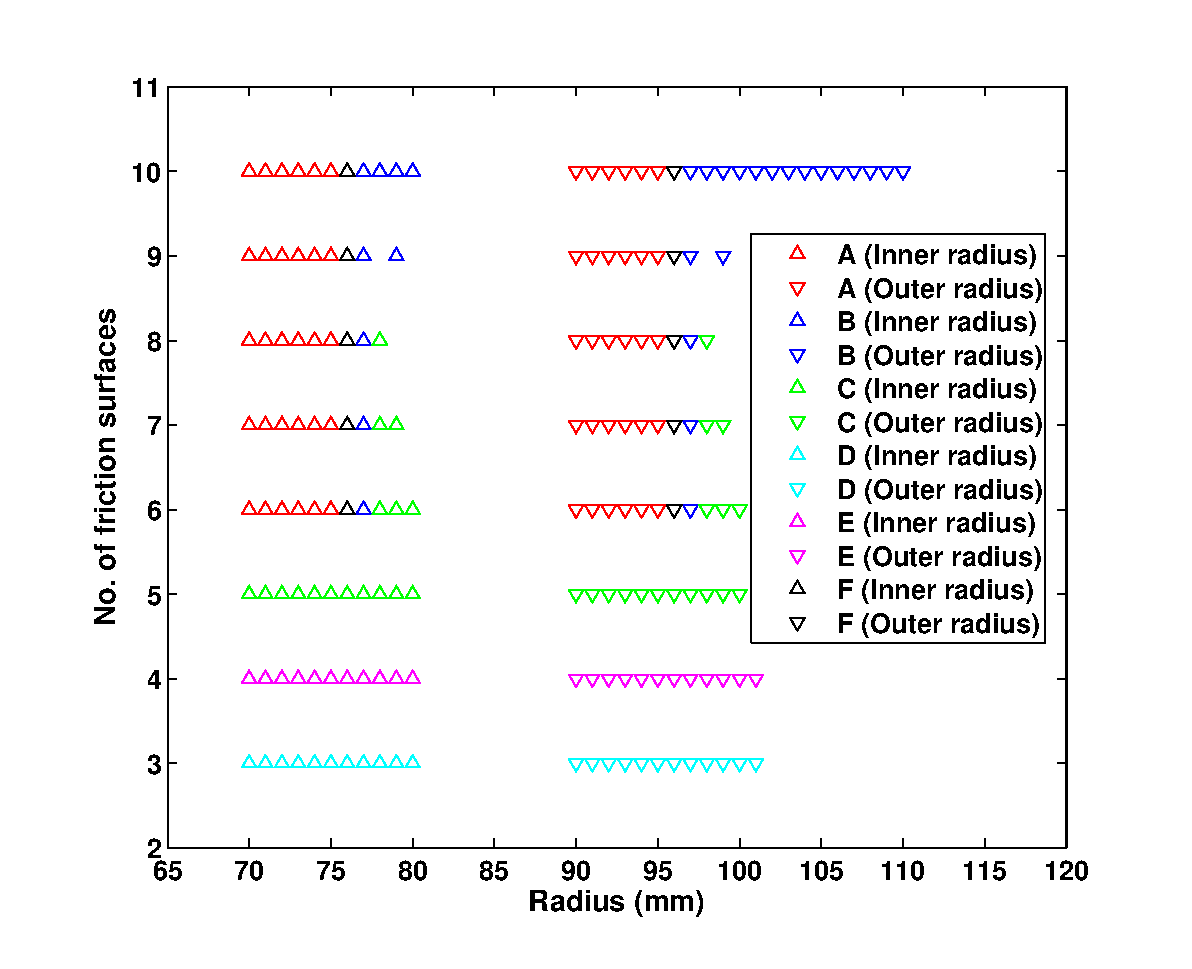
\includegraphics[width=100mm, height=80mm]{dia/clutchrVsZ.eps}
 \caption{Radius Vs. no. of friction surface plot for pareto-front
   clusters. Clusters \textbf{A}, \textbf{B}, \textbf{C} and \textbf{F} are
   distributed in four lines each while \textbf{D}, \textbf{E} and
   \textbf{F} are composed of single lines.}
 \label{clutchrVsZ}
\end{center}\end{figure}

The two dimensional nature of cluster \textbf{A} can be explained by this
plot. \textbf{A} has designs with small variation in radial dimensions
except in very heavy clutch brakes, those occupying the linear region in
plot \ref{clutch}. For the linear region designs, the number of disks is
maximum and the only way to design more powerful brakes is by increasing
the outer radius to increase the friction area. If the clustering had been
done in the design variables space only we would have clusters on the basis
of the number of contact surfaces only. Clustering in the combined
objective-decision variable space gives more meaningful clusters, which
have functionally similar designs.





\section{Analysis of welded beam design problem}
The NSGA-II run for the welded beam design problem yielded 500 solutions
with a population size of 500 running for 200 hundred generations. The
crossover and mutation probability were set to 0.73 and 0.53. After local
search the pareto-front obtained had 491 optimal solutions.  Figure
\ref{wbeam} shows the final pareto-front.


\begin{figure}[ht]\begin{center}
 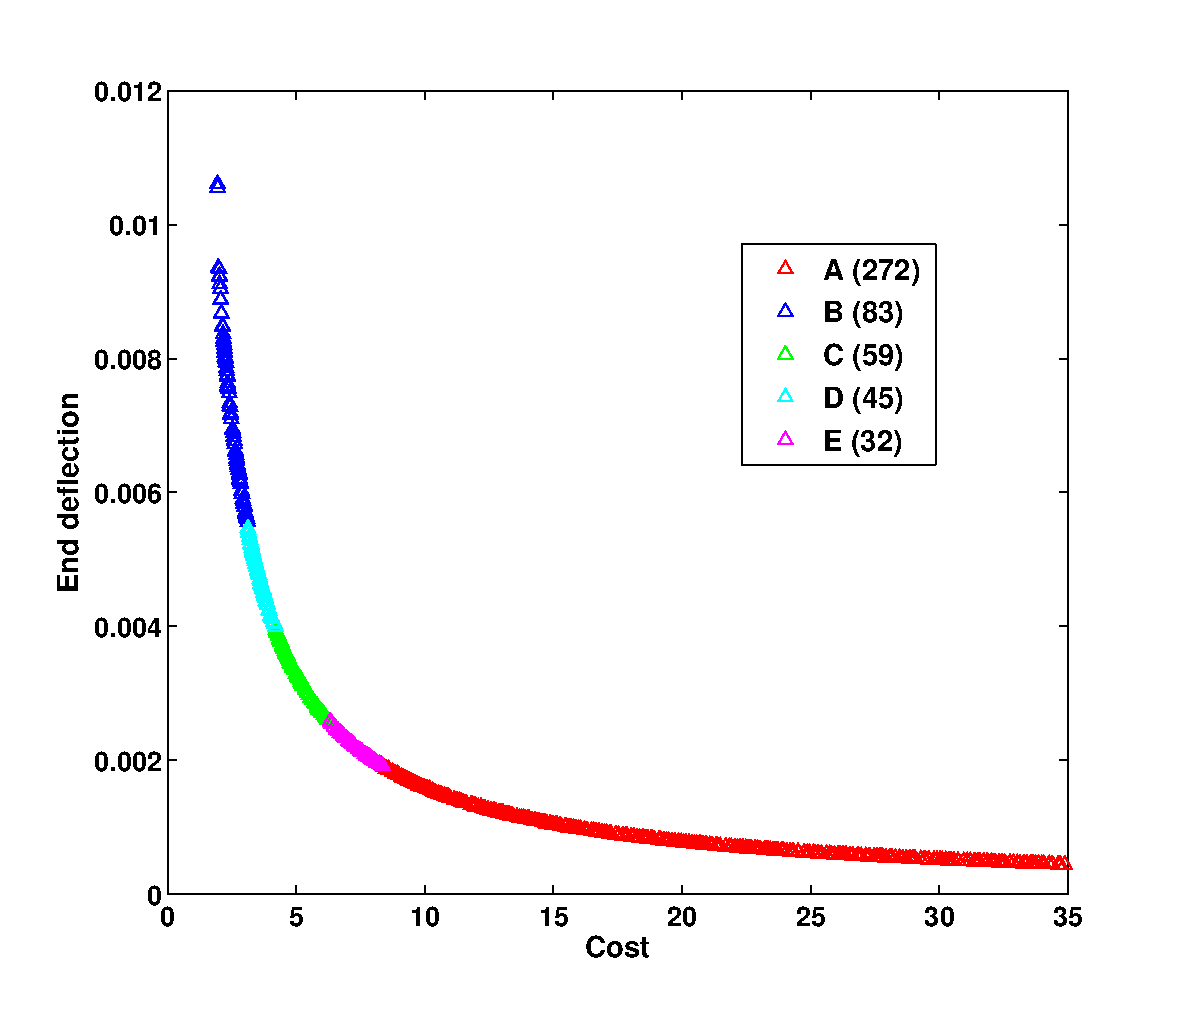
\includegraphics[width=100mm, height=80mm]{dia/wbeamParetoClusters.eps}
 \caption{Pareto-front and clusters of the welded beam design
   problem. Obtained with $k = 2$. The clusters in the extremes are the
   largest while those around the knee of the curve are relatively smaller}
 \label{wbeam}
\end{center}\end{figure}

\section{Isomap and PCA analysis of the pareto-front}

The residual variance plot shown in figure \ref{wbeamwrv} shows the largest
drop for dimension 2. Their is some further drop going from second two
third dimensional embedding. This indicates a manifold dimensionality of
one. The PCA explained variance (figure \ref{wbeamwev}) also shows only one
significant principal component with an explained variance of 93\%. Table
\ref{firstWbeamPC} shows the first principal component of the pareto-front.
The beam thickness ($b$) is the design variable with the highest weight in
the principal component. Weld thickness ($h$) and length of the weld ($l$)
have similar weights, albeit that of $l$ being in the reverse direction.
Width of the beam ($t$) is the least varying variable of all.

\begin{figure}[ht]\begin{center}
 \subfloat[Isomap Residual Variance for welded beam problem pareto-front]{
 \label{wbeamwrv} 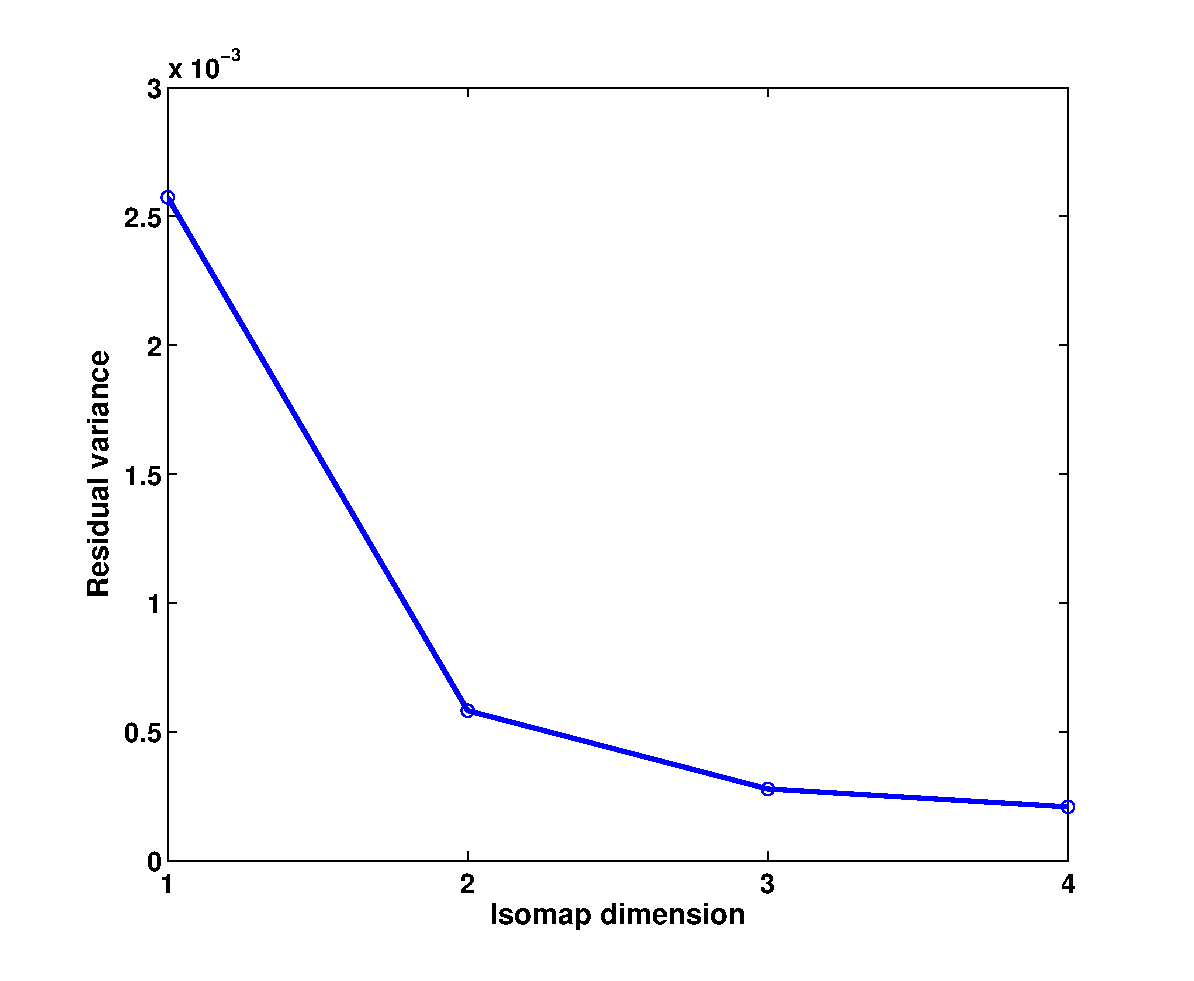
\includegraphics[width=62mm, height=52mm]{dia/wbeamWholeRV.eps}}
 \subfloat[PCA Explained variance for pareto-front of welded beam problem]{
 \label{wbeamwev} 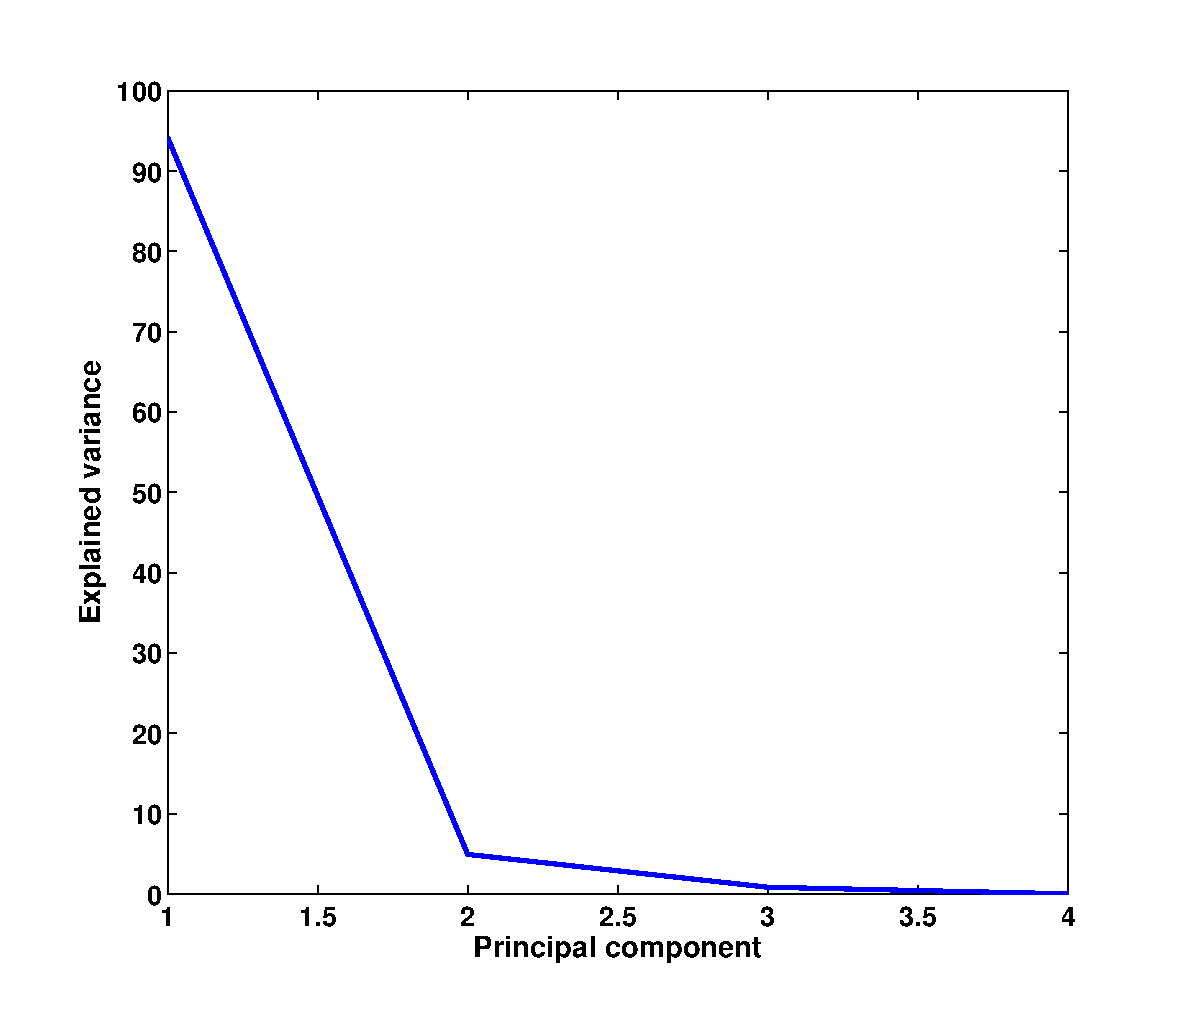
\includegraphics[width=62mm, height=52mm]{dia/wbeamWholeEV.eps}}
 \caption{Isomap and PCA results for the welded beam design problem}
 \label{wbeamWholeVar}
\end{center}\end{figure}


\begin{table}[!ht]
  \centering
  \begin{tabular}{c|c|c|c|c|}
    \cline{2-5}    
    & $b$ & $t$ & $l$  & $h$ \\
    \hline
    \multicolumn{1}{|c|}{First PC} & 0.903 & 0.001 & -0.278 & 0.325\\
    \hline
  \end{tabular}
  \caption{First two principal components of the clutch brake design problem pareto-front}
  \label{firstWbeamPC}
\end{table}


\subsection{Clustering analysis}
A large number of specific clusters could be obtained by suitably setting
the parameters of the algorithm, but we analyze only 5 clusters for the
sake of simplicity. The clusters are shown in figure \ref{wbeam}.

Clusters \textbf{A} and \textbf{B} have the largest number of optimal
solutions. They occupy the linear extremes of the pareto-front curve. Three
clusters are concentrated around the knee of the curve. Cluster \textbf{A}
has the costliest and sturdiest designs, while cluster \textbf{B} has the
cheapest and the weakest beams. Clusters \textbf{C}, \textbf{D} and
\textbf{E} have beams with mid range end deflection and cost.


\begin{figure}[ht]\begin{center}
 \subfloat[Isomap Residual Variances.]{
 \label{wbeamcrv} 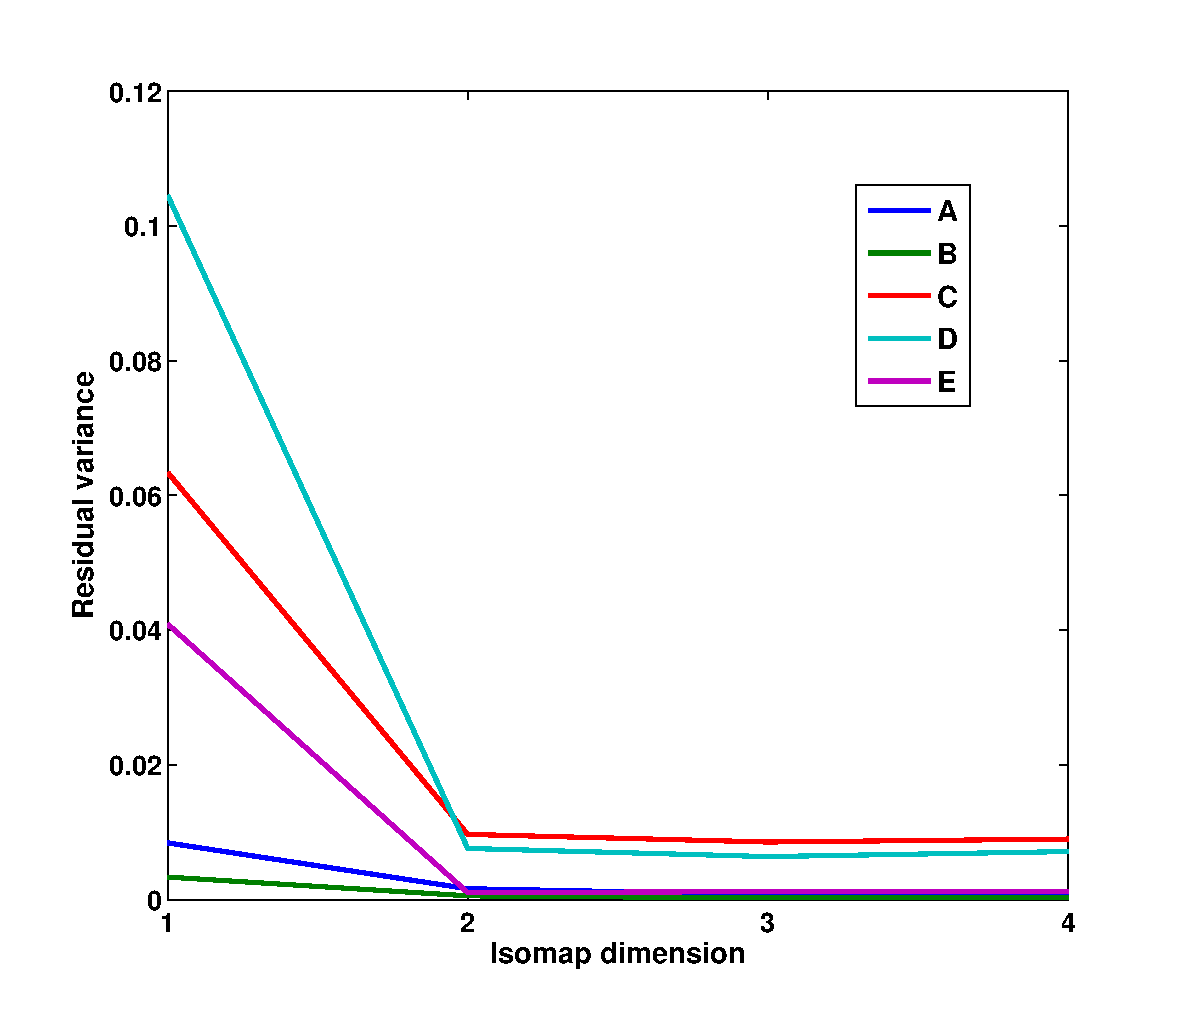
\includegraphics[width=62mm, height=52mm]{dia/wbeamClustersRV.eps}}
 \subfloat[PCA Explained variances.]{
 \label{wbeamcev} 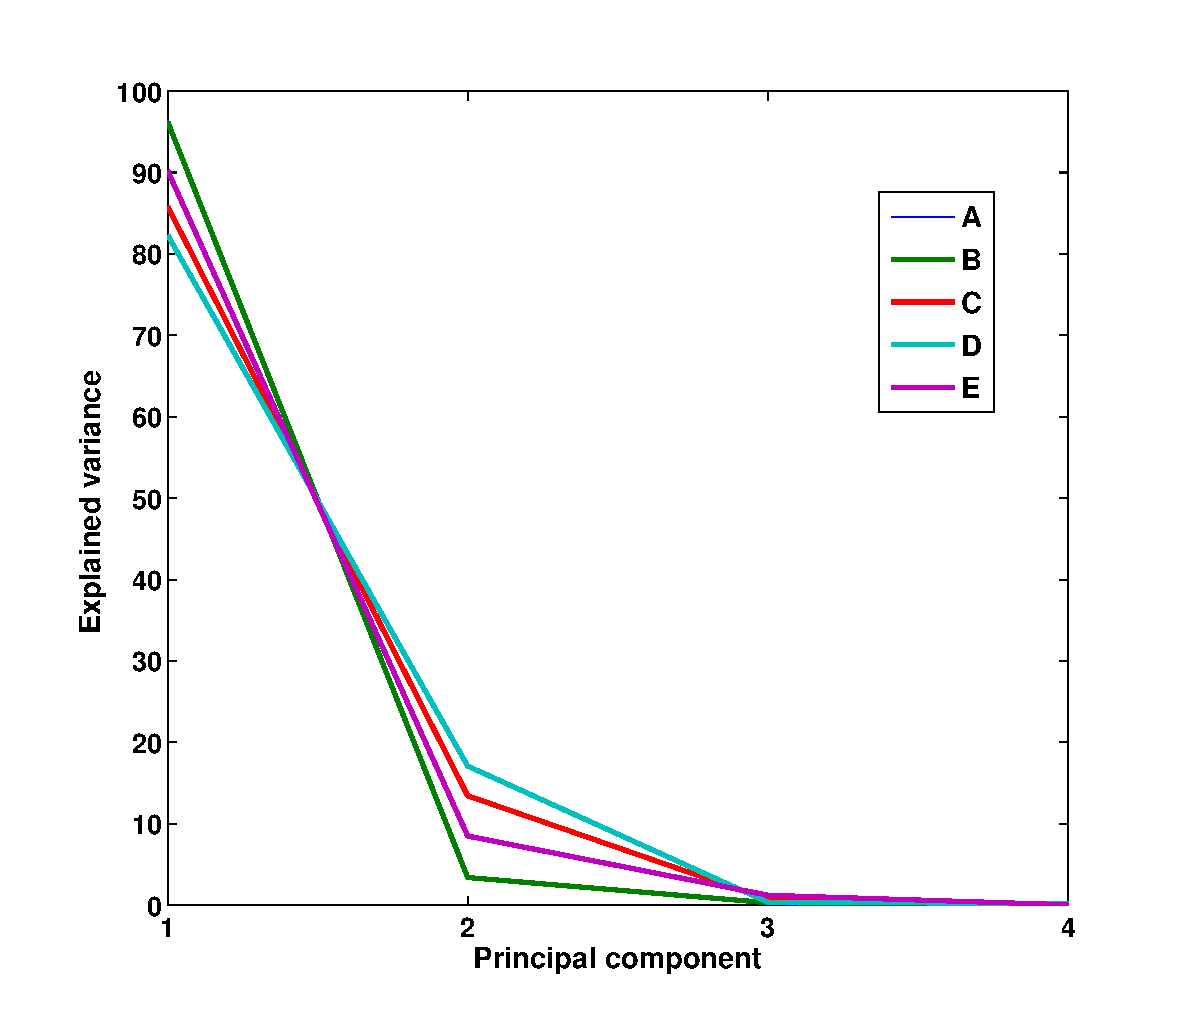
\includegraphics[width=62mm, height=52mm]{dia/wbeamClustersEV.eps}}
\caption{Isomap and PCA results for the clusters of welded beam design
  problem. All the clusters are one dimensional manifolds but clusters
  \textbf{C} and \textbf{D} have two linear dimensions as they have two
  significant components.}
 \label{wbeamClustersVar}
\end{center}\end{figure}

The Iosmap residual variances for all the clusters suggest one dimensional
manifolds clusters as all the curves have the largest drop for second
dimension. Clusters \textbf{D} and \textbf{C} have relatively higher
residual variances than other clusters. The PCA explained variance for
these clusters also show two significant components. The explained variance
plots for clusters \textbf{A} and \textbf{B} are almost the same resulting
in overlapping lines in the plot. The cluster E also has two significant
components.

Thickness of the beam ($b$) is the predominant variable in the principal
component of the cluster \textbf{A} (table \ref{first2wbeamPCs}) while
length of the weld ($l$) is the predominant variable in cluster
\textbf{B}. These two are at the two extremes of the pareto-front, the
former having designs with least deflection and highest cost and the latter
having cheapest designs with large end deflections. The clusters around the
knee of the pareto-front curve also have their two significant components
in the $b$ - $l$ plane with first component leaning more towards the $l$
direction and second component leaning towards $b$. For all the clusters
width of the beam ($t$) has the least variation. For all the optimal
designs, the width of the beam is approximately maximum possible value of
10.

% b - thickness of the beam
% t - width of the beam
% l - length of the weld
% h - thickness of the weld




\begin{table}[!ht]
  \centering
  \begin{tabular}{c|c|c|c|c|}
    \cline{2-5}
    & $b$ & $t$ & $ l$  & $h$ \\
    \hline
    \multicolumn{1}{|c|}{\textbf{A}} & 0.965 & 0 & -0.06 & 0.249 \\
    \hline
    \multicolumn{1}{|c|}{\textbf{B}} & 0.126 & 0.068 & -0.982 & 0.115\\
    \hline
    \multicolumn{1}{|c|}{\multirow{2}{*}{\textbf{C}}} & 0.435 & 0 & -0.755 & 0.488 \\ \cline{2-5}
    \multicolumn{1}{|c|}{}& 0.897 & 0.006 & 0.404 & -0.174\\
    \hline
    \multicolumn{1}{|c|}{\multirow{2}{*}{\textbf{D}}} & 0.309 & 0 & -0.883 & 0.351 \\ \cline{2-5}
    \multicolumn{1}{|c|}{}& 0.949 & 0.011 & 0.307 & -0.06\\
    \hline
    \multicolumn{1}{|c|}{\multirow{2}{*}{\textbf{E}}} & 0.381 & 0.002 & -0.616 & 0.688 \\ \cline{2-5}
    \multicolumn{1}{|c|}{}& 0.924 & 0.019 & 0.256 & -0.282\\
    \hline
  \end{tabular}
  \caption{Significant principal components of the pareto-front clusters of the welded beam design problem. The one dimensional clusters have $b$ and $l$ as the predominant variables. Two dimensional clusters also have their significant components in the $b$-$l$ plane. $t$ is the least varying variable in all the clusters.}
  \label{first2wbeamPCs}
\end{table}

\subsection{Discussion}
Width of the beam ($t$) variable has the least variation for all the
clusters. All the optimal designs use the maximum possible value of the
width beam. This suggests that a welded beam should be as wide as possible,
other design variables should be adjusted to obtain suitable designs. In
cluster \textbf{A} of the sturdiest designs, designs tend to vary in the
thickness of the beam the most with other variables limited to small ranges
of variation. The maximum value of $l$ an $h$ are 1.39 and 2.49 which are
significantly less than their maximum possible of 10 and 5
respectively. This suggests that increasing the size of the weld in $l$ and
$h$ beyond certain limit doesn't help in improving the sturdiness much,
though increasing thickness of the beam may improve the end deflection. In
cluster \textbf{B} the cost is minimum though the designs have larger end
deflection than in other clusters. In this cluster, $l$ is the variable
that varies the most, with other variables showing less variation. $l$ is
increased or decreased to increase or decrease the cost.

% b - thickness of the beam
% t - width of the beam
% l - length of the weld
% h - thickness of the weld







 

\chapter{Conclusion}


We have proposed a clustering and dimensionality reduction approach to
chunking in design tasks. A multi-objective optimization procedure is used
to first obtain a set of good designs, then clustering on the combined
objective-decision variable space is used to group the designs according to
their functional characteristics. Linear and non-linear dimensionality
reduction techniques are used to bring out the design implications of these
clusters and capture their semantics. We have applied this procedure to a
number of practical objective optimization problems and shown that majority
of the clusters obtained are one dimensional. In the examples considered
pareto frontiers that are two or higher dimensional manifolds, the
clustering neatly separated the higher dimensional patches of the manifold
into separate clusters.

This procedure could not only be used to learn design symbols in the
cognitive sense as discussed in \citep{mukerjee09}, but also to specialize
them further. For example, in BDCPMM design cluster \textbf{A} and
\textbf{B} would correspond to what the expert designer calls ``low end
designs'' (section \ref{bdcpmDiscuss}) and the cluster \textbf{C} to ``high
end designs''. This would provide a richer initial vocabulary to the system
with some interrelations among symbols already established.

The analysis of any decision task involves moving through several layers of
complexity. This suggests how a system can enrich already learnt symbols
through experience. Initially, the system could be presented with a minimal
multi-objective formulation (two objectives) of a design task. When the
system has learnt some initial symbols, a more detailed formulation with
possibly more objectives and a larger number of decision variables could be
presented to the system to gain ``experience''. The initial minimal
formulation would help establish the most pertinent principles, and the
gradual increase in complexity of the design task would help to bring out
the subtle and implicit relationships among the chunks. For example in the
gearbox design problem, the analysis of the fixed layout version of the
problem established the fact that thickness of the gear pairs in the last
transmission stage should go higher in accordance with the higher power
requirements, and the analysis of the complete problem brought to the front
some ideal combinations for no. of teeth in the final transmission
stage. However, the specification of the minimal initial formulation, and
the appropriate increase in complexity after each learning stage would
depend on the design task at hand.

We have shown the application the procedure to problems in design domain,
but such an approach to chunking is possible in any domain where the task
can be expressed as a multi-objective optimization. For example, in robot
path planning \citep{vadakkepat02}, many potential field functions are
optimized to calculate the optimal path for the robot. However,
optimization algorithms are complex and time consuming hence not suited for
real time application, but if a robot were to learn from the optimizations
as it calculates the optimal navigation path for a given situation, it
could use the readily available learnt information when faced with a
similar scenario next time. With increasing experience, such a system may
be able to learn chunks such as ``door'', ``connecting passage'',
``detours'' as components of high-level abstraction for important tasks.

Finally we return to the {\em chunk dimensionality conjecture}. In the five
examples considered the dimension of the chunk manifold is comparable to
the number of objectives. However as empirical validation, the sample set
is very small and clearly much work needs to be done to come up with a
theoretical basis for the conjecture.

Clearly the ramifications of such a conjecture are very high, especially in
the attempt to create machine models of expert behaviour. In this thesis we
have presented evidence that suggests that for many practical problems such
a conjecture may hold. This work may thus open the door for much greater
testing and validation in order to identify precisely the problem domains
where it may apply.





% \chapter{Application to other problems}
% In this chapter we present the results of our chunking and analysis
methodology on two problems. The first problem is the multiple disk clutch
brake design problem, a discreet optimization problem with five variables
and two objectives. The other is the welded beam design problem which is
continuous decision space problem with four variables and two objectives.

\section{Problem Introduction}
\subsection{Multiple-disk clutch brake design problem}


\begin{figure}[ht]\begin{center}
 \fbox{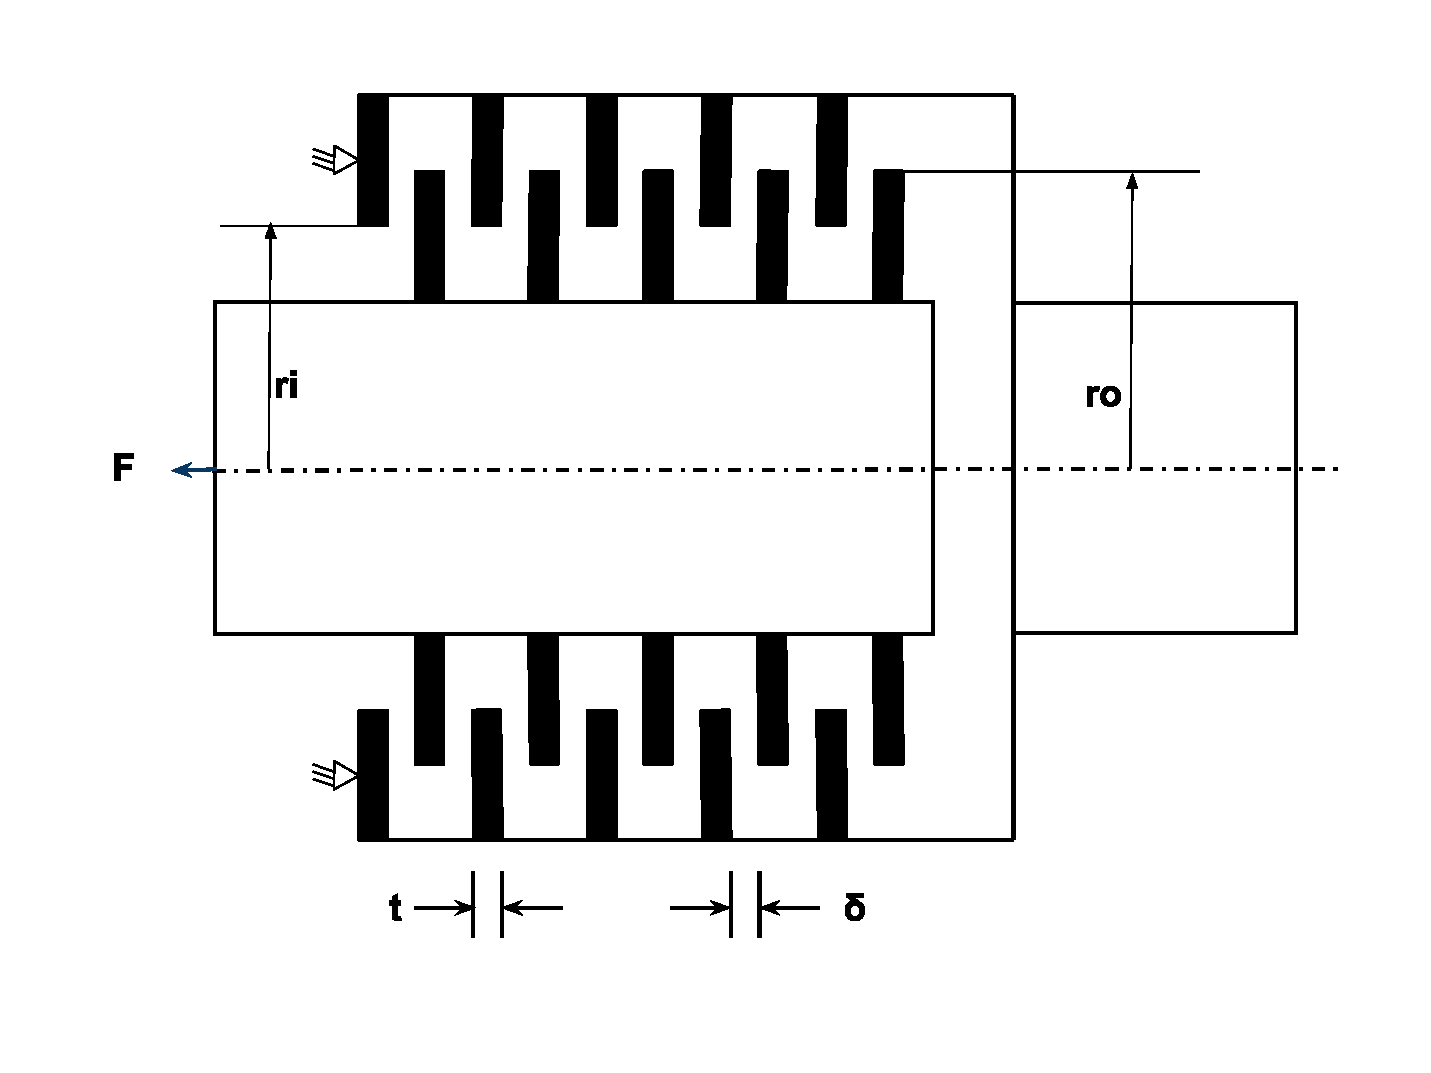
\includegraphics[width=75mm, height=60mm]{dia/clutchbrake.eps}}
 \caption{Schematics of a multiple disk clutch brake.}
 \label{clutchbrake}
\end{center}\end{figure}


We have adopted the problem specification used in \citep{deb06}. The
schematics of a multiple-disk clutch brake are shown in figure
\ref{clutchbrake}. Two conflicting objectives are considered in this 
optimization problem:
{\allowdisplaybreaks \begin{enumerate}
  \item minimization of mass, and,
  \item minimization of stopping time.
\end{enumerate}
This optimization problem is defined on five decision variables $\vec{x} = (r_i, r_o, t, F, Z)$, where:
\begin{enumerate}
  \item $r_i \in [60, 80]$ (in steps of one) is the inner radius in mm,
  \item $r_o \in [91, 110]$ (in steps of one) is the outer radius in mm,
  \item $t \in [1, 3]$ (in steps of 0.5) is the thickness of disks in mm,
  \item $F \in [600, 1000]$ (in steps of 10) is the actuating force in N and
  \item $Z \in [2, 10]$ (in steps of one) is the number of friction
    surfaces or disks.
\end{enumerate}}

The complete optimization problem is formulated as follows:

\begin{singlespacing}
\begin{flushleft}

{\allowdisplaybreaks
  \begin{align}
    \text{Maximize} \quad & f_1(\vec{x}) =  \pi (x_{2}^{2} - x_{1}^{2}) x_3 (x_5  + 1) \rho,\\
    \text{Minimize} \quad & f_2(\vec{x}) = T = \left. \frac{I_{z} \omega} {M_{h} + M_{f}} \right.,\\
    \text{Subject to,} & \nonumber \\
    \qquad &g1(\vec{x}) =  \left. x_2 - x_1 - \Delta R \geqslant 0 \right.,\\
    \qquad &g2(\vec{x}) = \left. L_{max} - (x_5 + 1)(x_3 + \delta) \geqslant 0 \right. \\
    \qquad &g3(\vec{x}) = \left. p_{max} - p_{rz} \geqslant 0 \right.\\
    \qquad &g4(\vec{x}) = \left. p_{max} V_{sr,max} - p_{rz} V_{sr} \geqslant 0 \right., \\
    \qquad &g5(\vec{x}) = \left. V_{sr, max} - V_{sr} \geqslant 0 \right., \\
    \qquad &g6(\vec{x}) = \left. M_{h} - s M_{s} \geqslant 0 \right., \\
    \qquad &g7(\vec{x}) = \left. T \geqslant 0 \right., \\
    \qquad &g8(\vec{x}) = \left. T_{max} - T \geqslant 0 \right.
  \end{align}
}

Where, 

\begin{itemize}
  \item $ M_h = \dfrac{2}{3} \mu x_4 x_5 \dfrac{x_{2}^3 - x_{1}^3}{x_2^2 - x_{1}^2} $ N.mm,
  \item $ \omega = \dfrac {\pi n}{30} $ rad/s ,
  \item $ A = \pi(x_2^2 - x_1^2) \quad \text{mm}^2$ ,
  \item $ p_{rz} = \dfrac{x_{4}}{A} \quad \text{N/mm}^2$,
  \item $ V_{sr} = \dfrac{\pi R_{sr} n} {30} $ mm/s ,
  \item $ R_{sr} = \dfrac{2}{3} \dfrac{x_{2}^3 - x_{1}^3}{x_2^2 - x_1^2} $ mm ,
  \item $ \Delta R = 20 $ mm ,
  \item $ L_{max} = 30 $ mm ,
  \item $ \mu = 0.5$ ,
  \item $p_{max} = 1 \quad \text{MPa}$, 
  \item $\rho = 0.0000078 \text{kg/mm}^3$,
  \item $V_{sr,max} = 10 \quad \text{m/s}$,
  \item $s = 1.5$,
  \item $T_{max} = 15 \quad \text{s}$, 
  \item $n = 250 \quad \text{rpm}$,
  \item $M_s = 40 \quad \text{Nm}$,
  \item $M_f = 3 \quad \text{Nm}$,
  \item $I_z = 55 \quad \text{kg.m}^2$,
  \item $\delta = 0.5 \quad \text{mm}$,
\end{itemize}

\end{flushleft}

\end{singlespacing}
    

\subsection{The welded beam design problem}



\begin{figure}[ht]\begin{center}
 \fbox{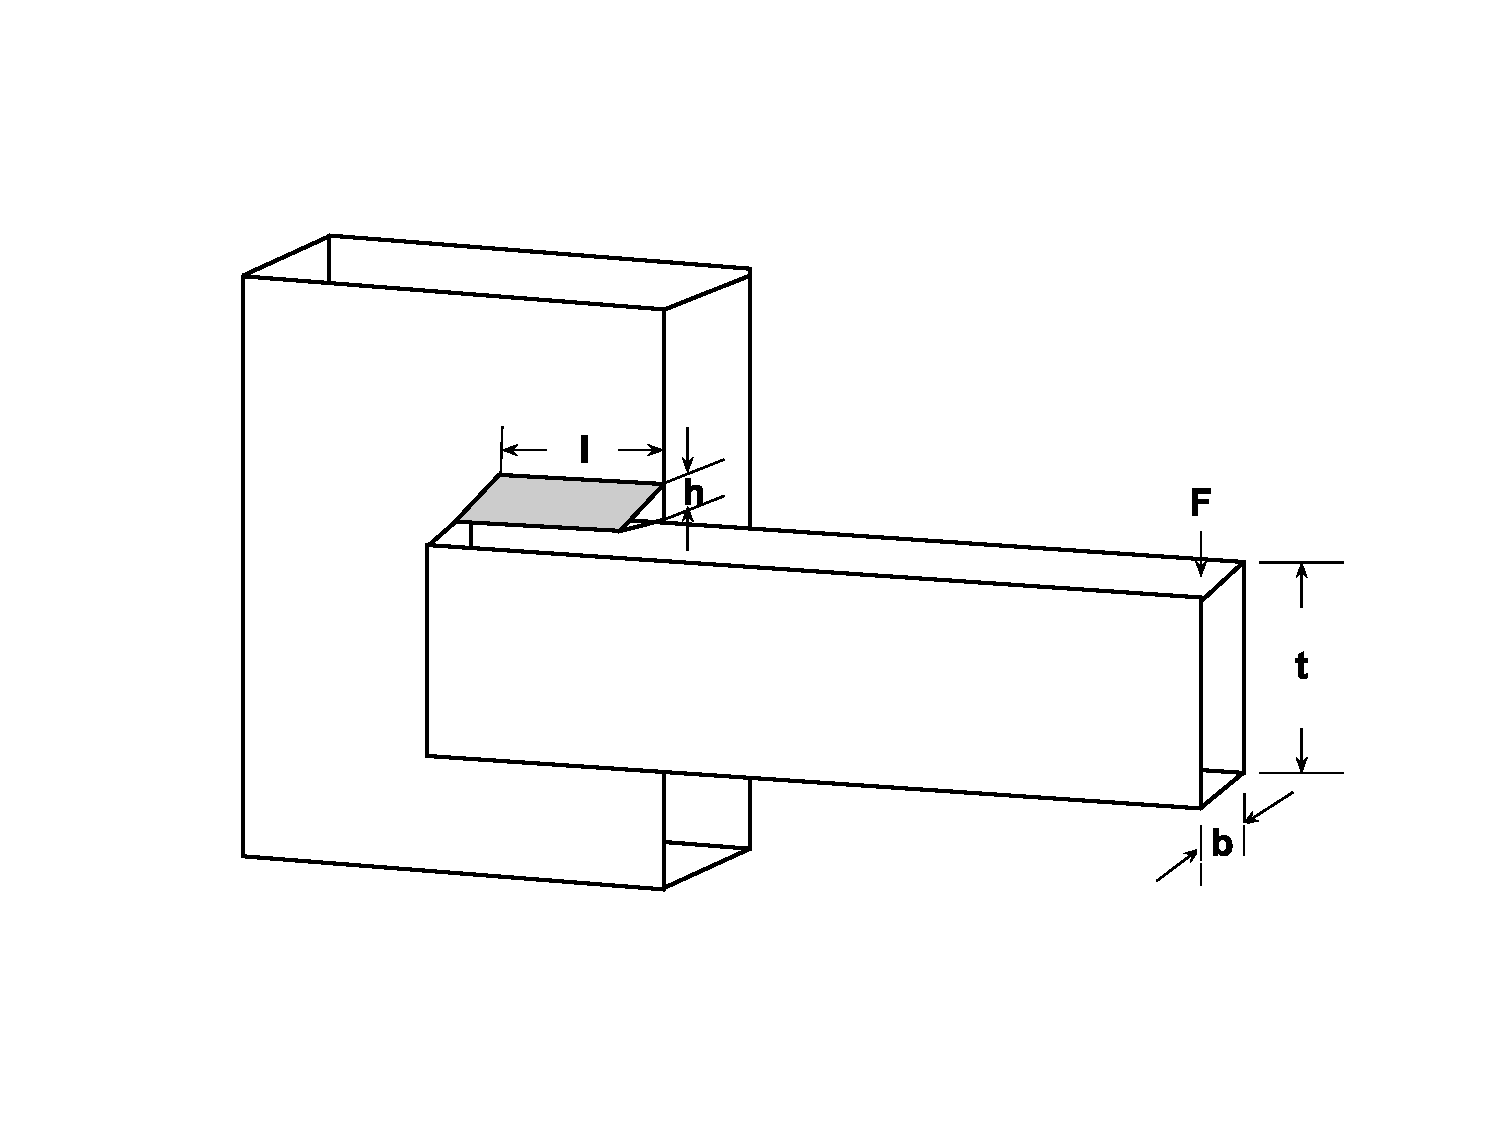
\includegraphics[width=75mm, height=60mm]{dia/wbeam.eps}}
 \caption{Schematics of a welded beam.}
 \label{wbeam}
\end{center}\end{figure}


Welded beam design problem is a well known Multi-objective optimization
problem. Here we adopt the formulation given in \citep{deb10}. The
objective of this problem is to minimize the cost and end deflection of a
beam welded at one end and supporting a load $ F = 6000$ lb at the other.
The overhang portion of the beam has a length of 14 in.There are four
design variables:
\begin{enumerate}
  \item $b \in [0.125, 5] $ thickness of the beam,
  \item $t \in [0.1, 10] $ width of the beam,
  \item $l \in [0.1, 10] $ length of the weld and
  \item $h \in [0.125, 5] $ thickness of the weld.
\end{enumerate}

The complete multi-objective formulation is as follows:

\begin{singlespacing}
  \begin{align}
    \text{Minimize} \quad &f_1(\vec{x}) = C = \left. 1.1047 h ^2 l + 0.04811 t b(14.0 + l) \right. \\
    \text{Minimize} \quad &f_2(\vec{x}) = D = \left. \dfrac{2.1952}{t^3 b} \right. \\
  \text{Subject to:}  & \nonumber \\
  \qquad &g_1(\vec{x}) = \left. 13600 - \tau (\vec{x}) \geqslant 0 \right. ,\\
  \qquad &g_2(\vec{x}) = \left. 30000 - \sigma (\vec{x}) \geqslant 0 \right.,\\
  \qquad &g_3(\vec{x}) = \left. b - h \geqslant 0 \right., \\
  \qquad &g_4(\vec{x}) = \left. P_c(\vec{x}) - 6000 \geqslant 0 \right. 
\end{align}

% \begin{align}
% \end{align}

Where,

\begin{itemize}
  \item $ \tau (\vec{x}) = \sqrt{ \dfrac{(\tau ')^2 + (\tau'')^2 + (l \tau' \tau'')} {\sqrt{ 0.25(l^2 + (h + t)^2)}}}$,
  \item $ \tau' = \dfrac {6000} {\sqrt{2} h l}$,
  \item $ \tau'' = \dfrac { 6000 (14 + 0.5l) \sqrt{0.25(l^2 + (h + t) ^2 )}} { 2 [0.707 h l (\frac{l^2}{12} + 0.25 (h + t) ^2)] } $,
  \item $ \sigma (\vec{x}) = \dfrac {504000} {t^2 b} $,
  \item $P_c (\vec{x}) = 64746.022(1-0.0282346t) t b^3$.
\end{itemize}

\end{singlespacing}    

\section{Analysis of the clutch brake design problem}

Figure \ref{clutch} shows the pareto-front obtained after running local
search on NSGA-II output. NSGA-II was run for 300 generations with a
population size of 5000 and yielded 125 near optimal solutions. The
probability for crossover and mutation were set to 0.79 and 0.5
respectively. Running local search gives a pareto-front consisting of 95
optimal solutions.

\begin{figure}[ht]\begin{center}
 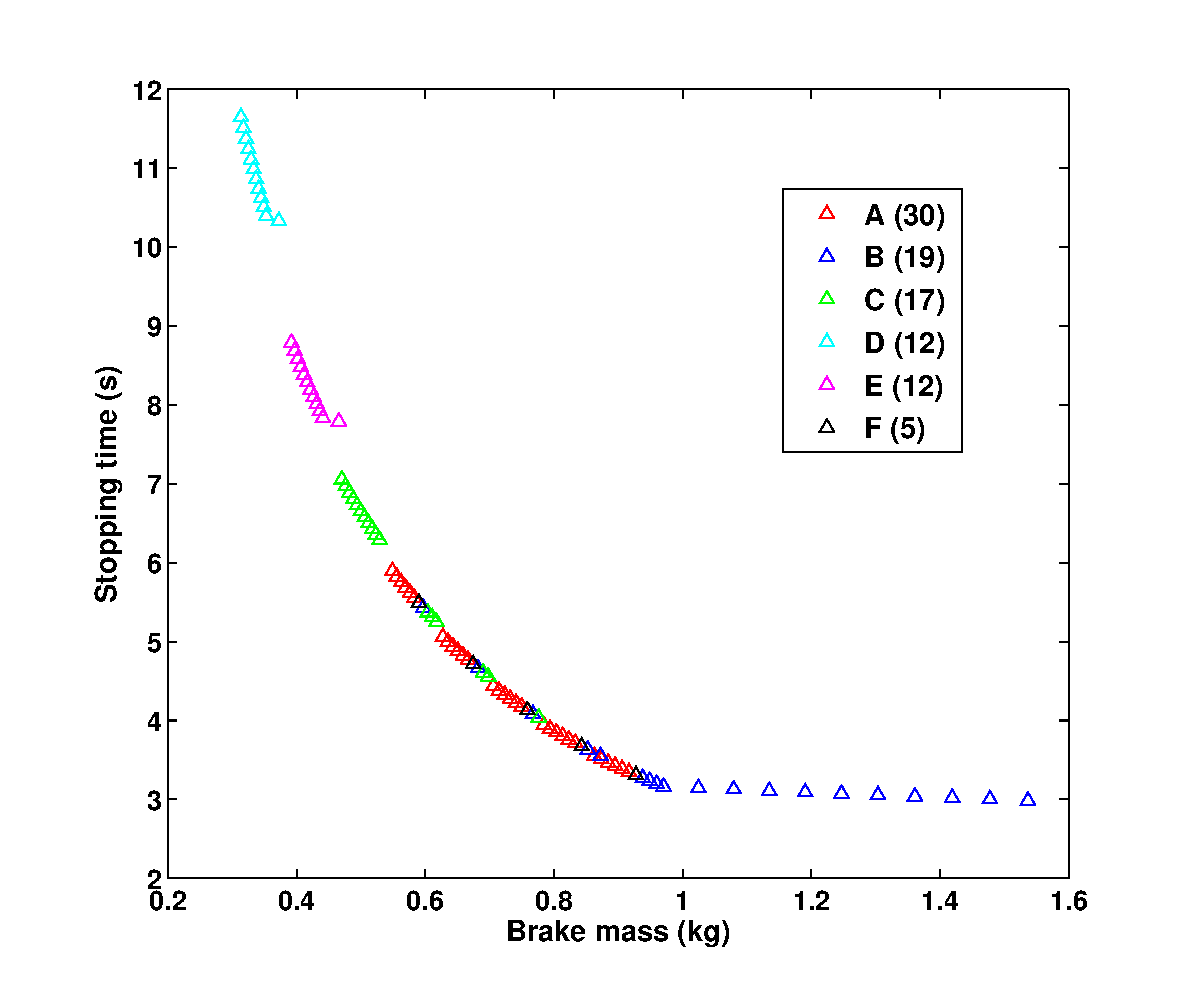
\includegraphics[width=100mm, height=80mm]{dia/clutchParetoClusters.eps}
 \caption{Pareto-front and the clusters of the multiple-disk clutch brake
   design problem. Clusters obtained with $k = 1.9$}
 \label{clutch}
\end{center}\end{figure}


\subsection{Isomap and PCA analysis of the pareto-front} 
Figure \ref{clutchwrv} and \ref{clutchwev} show the results of running
Isomap and PCA on the pareto-front of the clutch brake design problem. The
drop in the residual variance curve for the second Isomap dimension
indicates a manifold dimensionality of one. The PCA explained variance,
however, shows two principal components with significant explained
variances, the first with 80\% explained variance and the second with 17\%.


\begin{figure}[ht]\begin{center}
 \subfloat[Isomap Residual Variance.]{
 \label{clutchwrv} 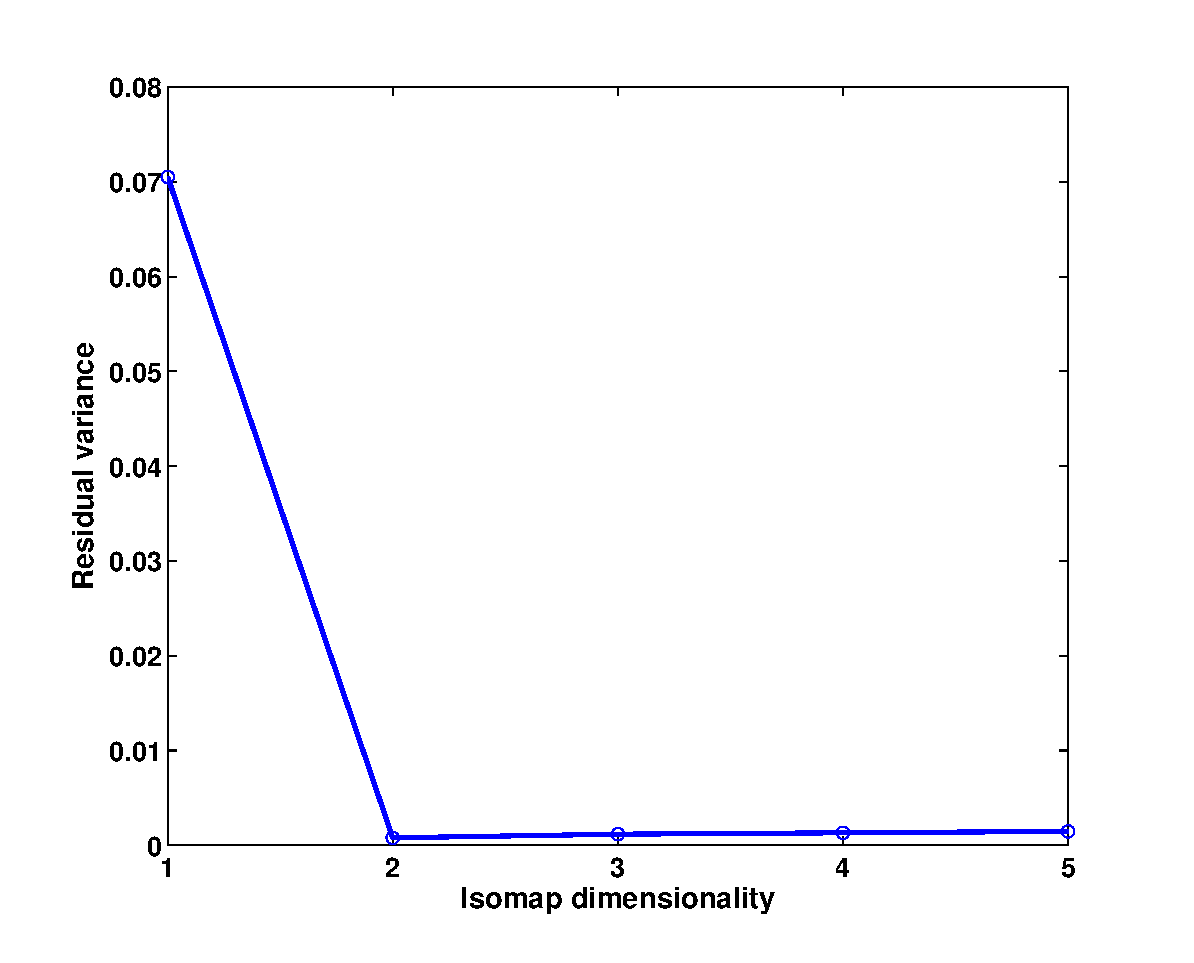
\includegraphics[width=62mm, height=52mm]{dia/clutchRV.eps}}
 \subfloat[PCA Explained variance.]{
 \label{clutchwev} 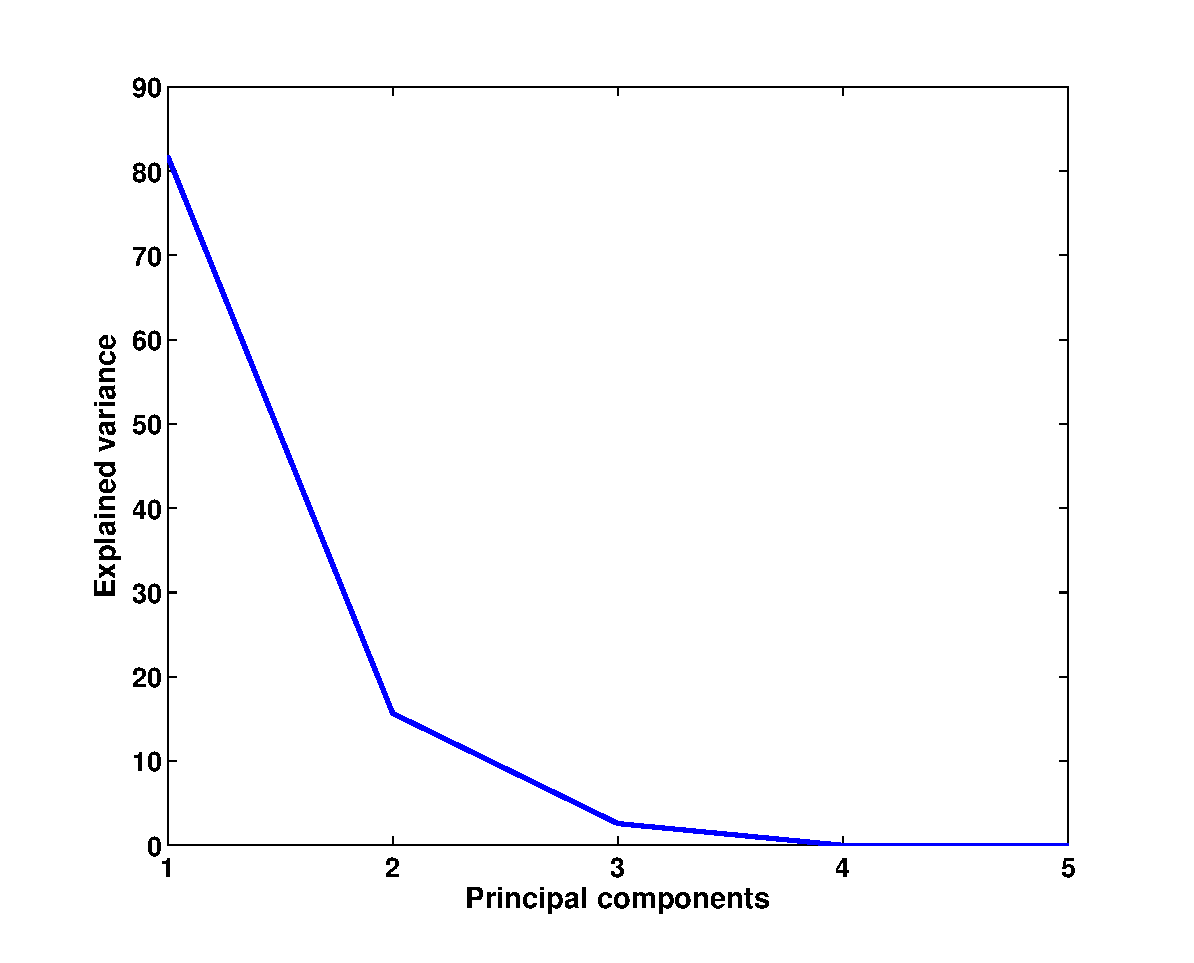
\includegraphics[width=62mm, height=52mm]{dia/clutchEV.eps}}
\caption{Isomap and PCA results for the pareto-front of multiple-disk
  clutch brake problem pareto-front. The manifold dimensionality is one as
  indicated in the Isomap residual variance plot but the PCA explained
  variance shows two significant principal components.}
 \label{clutchWholeVar}
\end{center}\end{figure}

Table \ref{first2clutchPCs} shows the first two significant components of
the pareto-front. Outer radius ($r_o$) has the highest weight in the
first principal component followed by inner radius ($r_i$). The number of
surfaces also has some variation. In the second principal component number
of surfaces ($Z$) is the dominant variable followed by inner radius with a
small weight. The variables thickness ($t$) and actuating force ($F$)
have zero weights in both the significant principal components indicating
they have the same values for all the optimal solutions. The thickness and
actuating force are fixed at the minimum and maximum possible values of 1
and 1000 respectively for all the optimal solutions.


\begin{table}[!ht]
  \centering
  \begin{tabular}{c|c|c|c|c|c|}
    \cline{2-6}
    & $r_{i}$ & $r_{o}$ & $ t $  & $F$ & $Z$ \\
    \hline
    \multicolumn{1}{|c|}{First PC} & 0.578 & 0.806 & 0 & 0 & 0.119\\
    \hline
    \multicolumn{1}{|c|}{Second PC} & -0.207 & 0.004 & 0 & 0 & 0.978\\
    \hline
  \end{tabular}
  \caption{First two principal components of the clutch brake design problem pareto-fron}
  \label{first2clutchPCs}
\end{table}

\subsection{Clustering analysis}
The pareto-front of this problem has a small number (95) of optimal
solutions. The $k$ parameter of the clustering algorithm had to be adjusted
accordingly to obtain a proper distribution of points in clusters. Six
clusters were obtained with $k = 1.9$. The clusters are shown in figure
\ref{clutch}.

Cluster \textbf{A} is the largest cluster with 37 points. It has the
mid-range designs of the clutch brake with stopping times ranging from 3.2
seconds to 6 seconds. Cluster \textbf{B} is composed of the heaviest and
most powerful brake designs, apart from some mid-range designs. It's the
only cluster having designs with weights in excess of 1 kg. Below 1 kg
designs follow a parabolic time vs. weight characteristics, but above 1 kg
designs show a linear relationship, an increase in weight yielding very
little benefit in stopping time. Clusters \textbf{D} and \textbf{E} have
the low end designs with stopping times in excess of 7.5 s. These are the
only clusters that appear as single contiguous chunks in the
pareto-front. Clusters \textbf{A}, \textbf{B}, \textbf{C} and \textbf{E}
have designs in overlapping objective ranges.

Isomap residual variances of the clusters (figure \ref{clutchcrv})
indicate one dimensional manifolds for the clusters, similar to the whole
pareto-front. This verifies the claims of the {\em chunk dimensionality
  conjecture} (section \ref{cdc}). Clusters \textbf{B-C} and \textbf{D-E}
have exactly same residual variances.  Cluster \textbf{A} has the highest
error in reverse mapping the one dimensional Isomap embedding. Clusters
\textbf{D} and \textbf{E} have negligible residual variances. PCA explained
variances for the clusters (figure \ref{clutchcev}) show a single
significant principal component for all the clusters except cluster
\textbf{A}.


\begin{figure}[ht]\begin{center}
 \subfloat[Isomap Residual Variance.]{
 \label{clutchcrv} 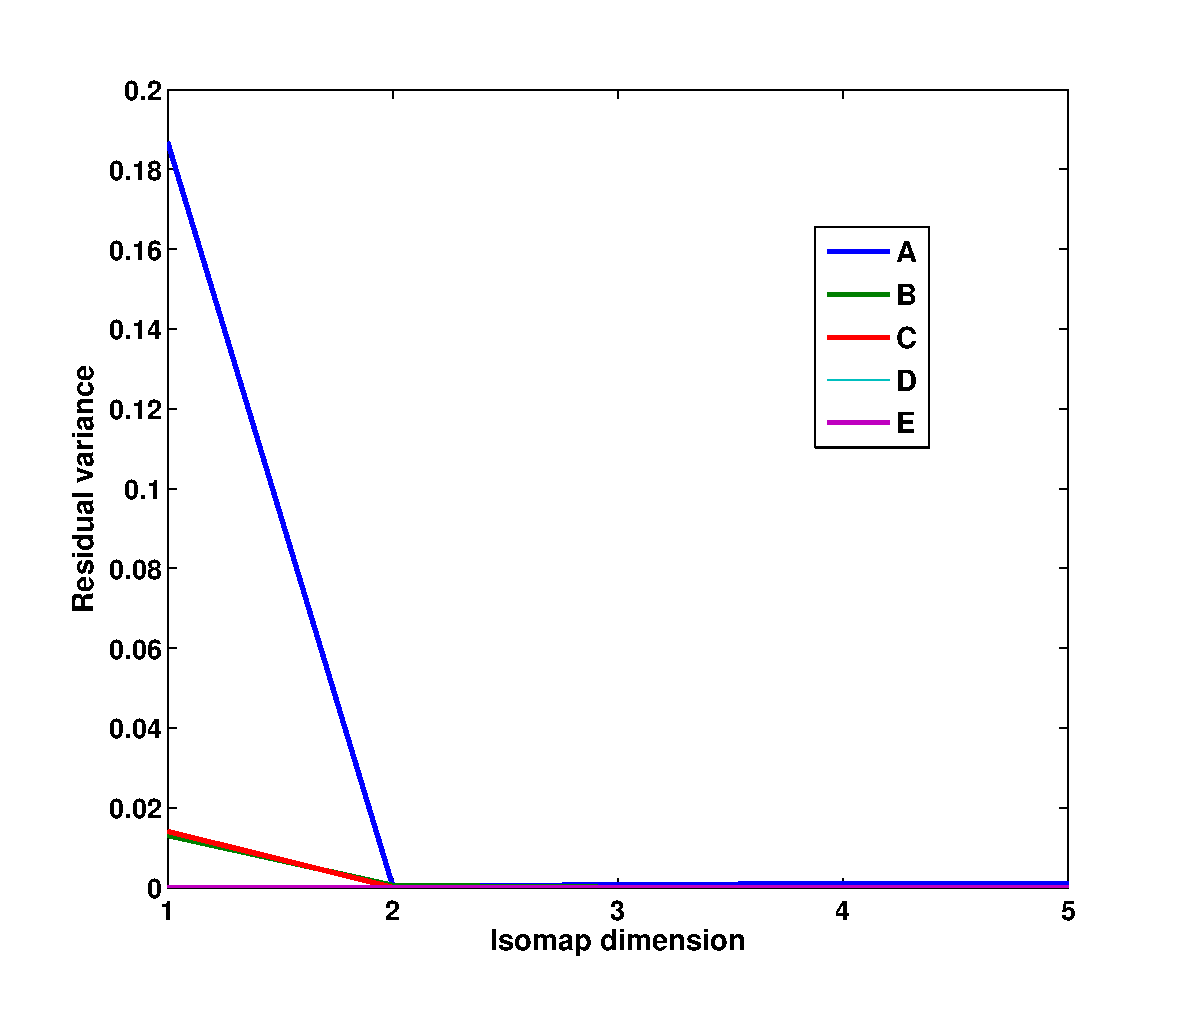
\includegraphics[width=62mm, height=52mm]{dia/clutchClustersRV.eps}}
 \subfloat[PCA Explained variance.]{
 \label{clutchcev} 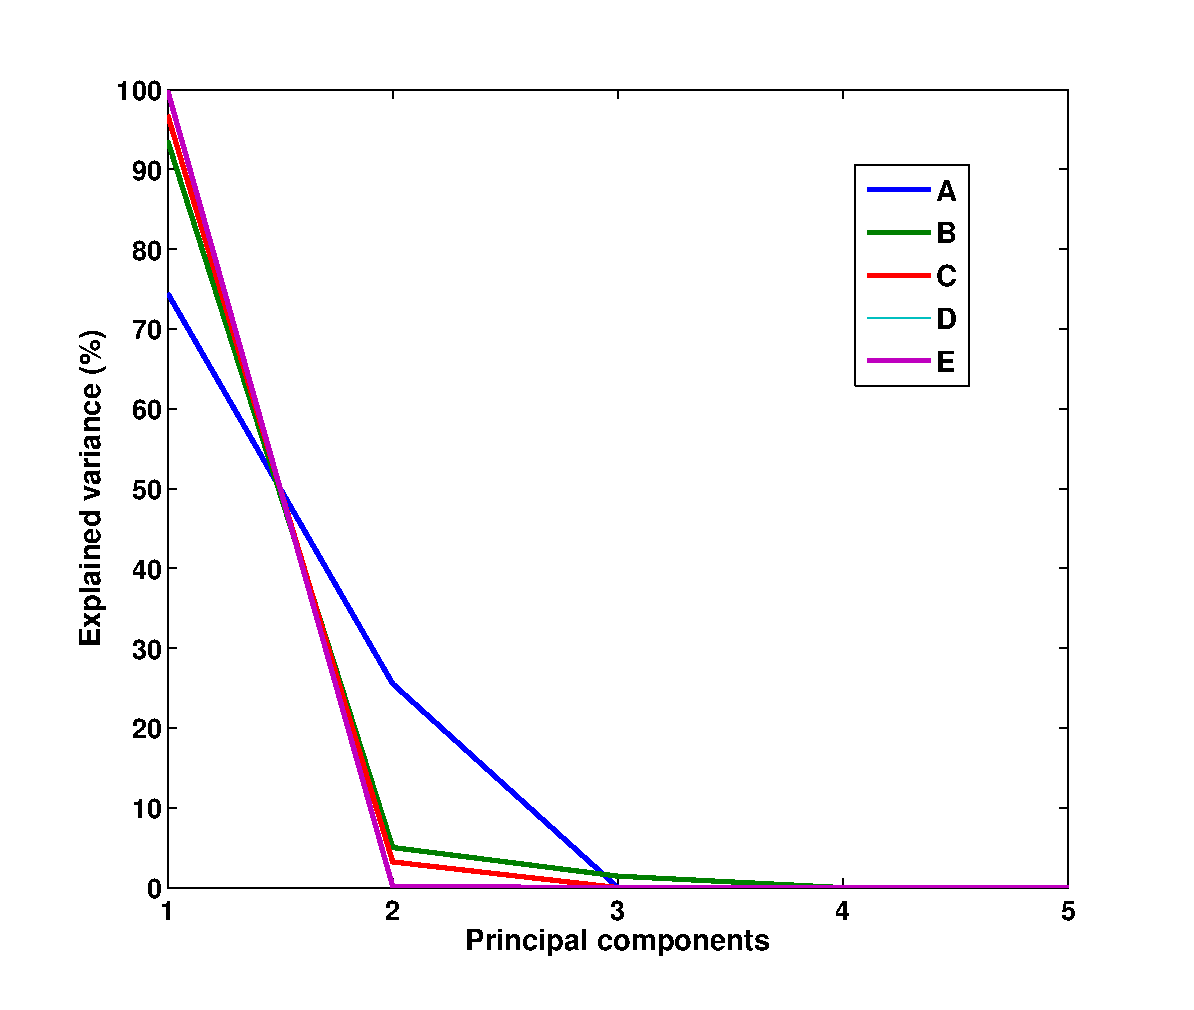
\includegraphics[width=62mm, height=52mm]{dia/clutchClustersEV.eps}}
\caption{Isomap and PCA results for the clusters of multiple-disk clutch
  brake problem. The manifold dimensionality of all the clusters is one,
  though cluster \textbf{A} has linear dimensionality of two indicated by
  two significant principal components in its explained variance plot.}
 \label{clutchClustersVar}
\end{center}\end{figure}


\begin{table}[!ht]
  \centering
  \begin{tabular}{c|c|c|c|c|c|}
    \cline{2-6}
    & $r_{i}$ & $r_{o}$ & $ t $  & $F$ & $Z$ \\
    \hline
    \multicolumn{1}{|c|}{\multirow{2}{*}{\textbf{A}}} & 0.707 & 0.707 & 0 & 0 & 0\\ \cline{2-6}
    \multicolumn{1}{|c|}{}& 0 & 0 & 0 & 0 & 1\\
    \hline
    \multicolumn{1}{|c|}{\textbf{B}} & 0.236 & 0.960 & 0 & 0 & 0.146\\
    \hline
    \multicolumn{1}{|c|}{\textbf{C}} & 0.703 & 0.703 & 0 & 0 & 0.097\\
    \hline
    \multicolumn{1}{|c|}{\textbf{D}} & 0.694 & 0.719 & 0 & 0 & 0\\
    \hline
    \multicolumn{1}{|c|}{\textbf{E}} & 0.694 & 0.719 & 0 & 0 & 0\\
    \hline
    \multicolumn{1}{|c|}{\textbf{F}} & 0 & 0 & 0 & 0 & 1\\
    \hline
  \end{tabular}
  \caption{Significant principal components of the clutch brake design problem clusters. $t$ and $F$ have no weights in any principal component. The inner and outer radii($r_i$ and $r_o$) show the highest variation for each cluster. The second component is parallel to the {\em number of friction surfaces (Z)} dimension.}
  \label{first2clutchPCs}
\end{table}

Table \ref{first2clutchPCs} shows the principal components of the
clusters. For most of the clusters, the radius variables have similar
weights. In cluster \textbf{B} the outer radius has higher weight than the
inner radius.  The second principal component of cluster \textbf{A} has
entirely composed of a single variable $Z$ only. Clusters \textbf{D} and
\textbf{E} have exactly the same components. The cluster \textbf{F} has 
variable $Z$ as its single Principal component.

\subsection{Discussion}

The most important fact that comes out of this analysis is that all optimal
clutch brakes should be designed with disks with smallest possible
thickness.  Secondly, a clutch brake must be designed for maximum actuating
force only, since the stopping time is inversely proportional to the
actuating force. The stopping time is also dependent on the friction area
as is evident from the figure \ref{clutchrVsZ}. A higher outer radius and a
larger number of friction surfaces (no. of disks) allow for a larger
contact area, but increasing the number of disks also increases the weight
of the design.  This trade-off is visible in all the clusters. The fact
that radius variables show greater variation across all clusters suggests
that to reduce the stopping time increasing the radial dimension is the
more economical option.


\begin{figure}[ht]\begin{center}
 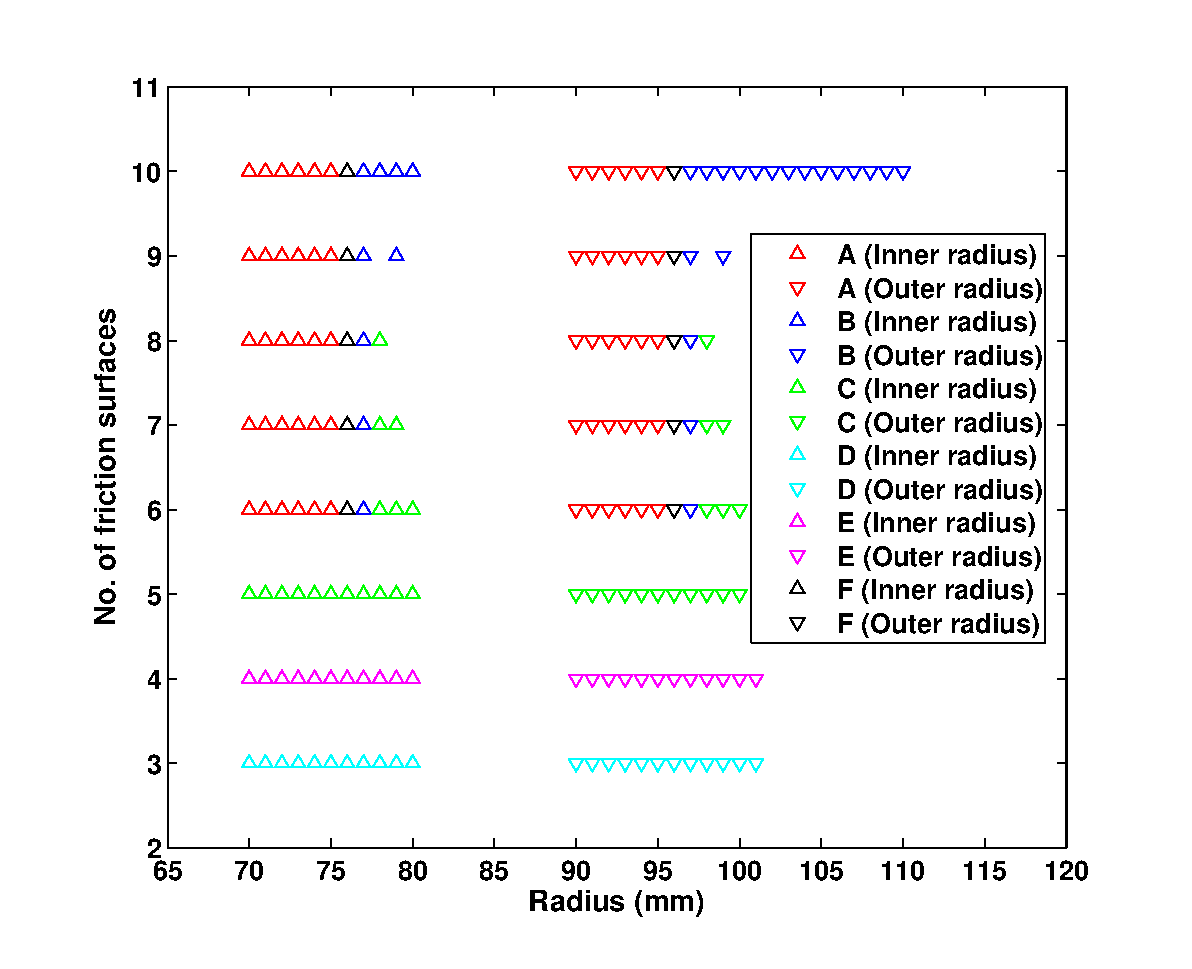
\includegraphics[width=100mm, height=80mm]{dia/clutchrVsZ.eps}
 \caption{Radius Vs. no. of friction surface plot for pareto-front
   clusters. Clusters \textbf{A}, \textbf{B}, \textbf{C} and \textbf{F} are
   distributed in four lines each while \textbf{D}, \textbf{E} and
   \textbf{F} are composed of single lines.}
 \label{clutchrVsZ}
\end{center}\end{figure}

The two dimensional nature of cluster \textbf{A} can be explained by this
plot. \textbf{A} has designs with small variation in radial dimensions
except in very heavy clutch brakes, those occupying the linear region in
plot \ref{clutch}. For the linear region designs, the number of disks is
maximum and the only way to design more powerful brakes is by increasing
the outer radius to increase the friction area. If the clustering had been
done in the design variables space only we would have clusters on the basis
of the number of contact surfaces only. Clustering in the combined
objective-decision variable space gives more meaningful clusters, which
have functionally similar designs.





\section{Analysis of welded beam design problem}
The NSGA-II run for the welded beam design problem yielded 500 solutions
with a population size of 500 running for 200 hundred generations. The
crossover and mutation probability were set to 0.73 and 0.53. After local
search the pareto-front obtained had 491 optimal solutions.  Figure
\ref{wbeam} shows the final pareto-front.


\begin{figure}[ht]\begin{center}
 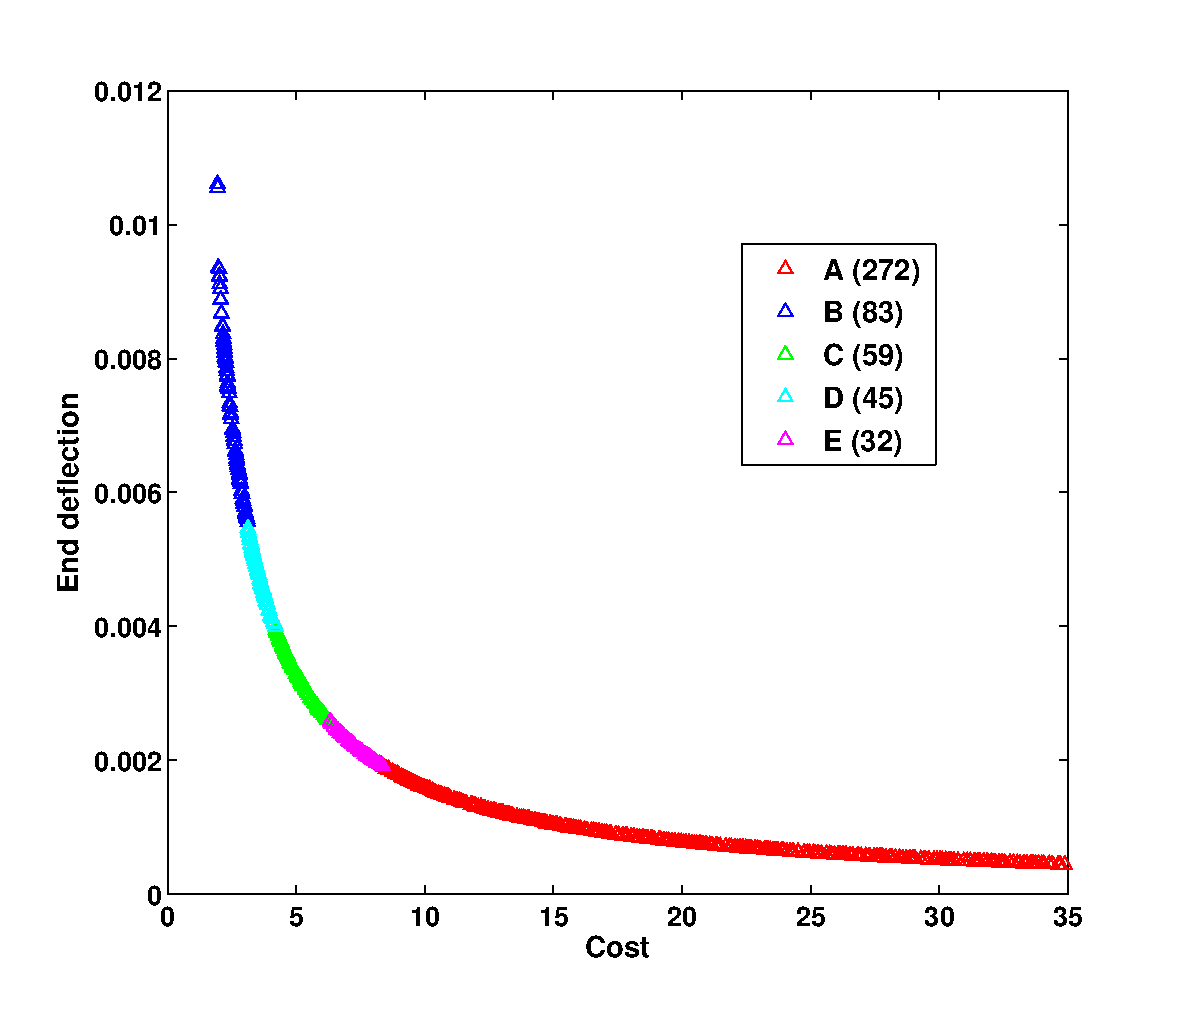
\includegraphics[width=100mm, height=80mm]{dia/wbeamParetoClusters.eps}
 \caption{Pareto-front and clusters of the welded beam design
   problem. Obtained with $k = 2$. The clusters in the extremes are the
   largest while those around the knee of the curve are relatively smaller}
 \label{wbeam}
\end{center}\end{figure}

\section{Isomap and PCA analysis of the pareto-front}

The residual variance plot shown in figure \ref{wbeamwrv} shows the largest
drop for dimension 2. Their is some further drop going from second two
third dimensional embedding. This indicates a manifold dimensionality of
one. The PCA explained variance (figure \ref{wbeamwev}) also shows only one
significant principal component with an explained variance of 93\%. Table
\ref{firstWbeamPC} shows the first principal component of the pareto-front.
The beam thickness ($b$) is the design variable with the highest weight in
the principal component. Weld thickness ($h$) and length of the weld ($l$)
have similar weights, albeit that of $l$ being in the reverse direction.
Width of the beam ($t$) is the least varying variable of all.

\begin{figure}[ht]\begin{center}
 \subfloat[Isomap Residual Variance for welded beam problem pareto-front]{
 \label{wbeamwrv} \includegraphics[width=62mm, height=52mm]{dia/wbeamWholeRV.eps}}
 \subfloat[PCA Explained variance for pareto-front of welded beam problem]{
 \label{wbeamwev} \includegraphics[width=62mm, height=52mm]{dia/wbeamWholeEV.eps}}
 \caption{Isomap and PCA results for the welded beam design problem}
 \label{wbeamWholeVar}
\end{center}\end{figure}


\begin{table}[!ht]
  \centering
  \begin{tabular}{c|c|c|c|c|}
    \cline{2-5}    
    & $b$ & $t$ & $l$  & $h$ \\
    \hline
    \multicolumn{1}{|c|}{First PC} & 0.903 & 0.001 & -0.278 & 0.325\\
    \hline
  \end{tabular}
  \caption{First two principal components of the clutch brake design problem pareto-front}
  \label{firstWbeamPC}
\end{table}


\subsection{Clustering analysis}
A large number of specific clusters could be obtained by suitably setting
the parameters of the algorithm, but we analyze only 5 clusters for the
sake of simplicity. The clusters are shown in figure \ref{wbeam}.

Clusters \textbf{A} and \textbf{B} have the largest number of optimal
solutions. They occupy the linear extremes of the pareto-front curve. Three
clusters are concentrated around the knee of the curve. Cluster \textbf{A}
has the costliest and sturdiest designs, while cluster \textbf{B} has the
cheapest and the weakest beams. Clusters \textbf{C}, \textbf{D} and
\textbf{E} have beams with mid range end deflection and cost.


\begin{figure}[ht]\begin{center}
 \subfloat[Isomap Residual Variances.]{
 \label{wbeamcrv} \includegraphics[width=62mm, height=52mm]{dia/wbeamClustersRV.eps}}
 \subfloat[PCA Explained variances.]{
 \label{wbeamcev} \includegraphics[width=62mm, height=52mm]{dia/wbeamClustersEV.eps}}
\caption{Isomap and PCA results for the clusters of welded beam design
  problem. All the clusters are one dimensional manifolds but clusters
  \textbf{C} and \textbf{D} have two linear dimensions as they have two
  significant components.}
 \label{wbeamClustersVar}
\end{center}\end{figure}

The Iosmap residual variances for all the clusters suggest one dimensional
manifolds clusters as all the curves have the largest drop for second
dimension. Clusters \textbf{D} and \textbf{C} have relatively higher
residual variances than other clusters. The PCA explained variance for
these clusters also show two significant components. The explained variance
plots for clusters \textbf{A} and \textbf{B} are almost the same resulting
in overlapping lines in the plot. The cluster E also has two significant
components.

Thickness of the beam ($b$) is the predominant variable in the principal
component of the cluster \textbf{A} (table \ref{first2wbeamPCs}) while
length of the weld ($l$) is the predominant variable in cluster
\textbf{B}. These two are at the two extremes of the pareto-front, the
former having designs with least deflection and highest cost and the latter
having cheapest designs with large end deflections. The clusters around the
knee of the pareto-front curve also have their two significant components
in the $b$ - $l$ plane with first component leaning more towards the $l$
direction and second component leaning towards $b$. For all the clusters
width of the beam ($t$) has the least variation. For all the optimal
designs, the width of the beam is approximately maximum possible value of
10.

% b - thickness of the beam
% t - width of the beam
% l - length of the weld
% h - thickness of the weld




\begin{table}[!ht]
  \centering
  \begin{tabular}{c|c|c|c|c|}
    \cline{2-5}
    & $b$ & $t$ & $ l$  & $h$ \\
    \hline
    \multicolumn{1}{|c|}{\textbf{A}} & 0.965 & 0 & -0.06 & 0.249 \\
    \hline
    \multicolumn{1}{|c|}{\textbf{B}} & 0.126 & 0.068 & -0.982 & 0.115\\
    \hline
    \multicolumn{1}{|c|}{\multirow{2}{*}{\textbf{C}}} & 0.435 & 0 & -0.755 & 0.488 \\ \cline{2-5}
    \multicolumn{1}{|c|}{}& 0.897 & 0.006 & 0.404 & -0.174\\
    \hline
    \multicolumn{1}{|c|}{\multirow{2}{*}{\textbf{D}}} & 0.309 & 0 & -0.883 & 0.351 \\ \cline{2-5}
    \multicolumn{1}{|c|}{}& 0.949 & 0.011 & 0.307 & -0.06\\
    \hline
    \multicolumn{1}{|c|}{\multirow{2}{*}{\textbf{E}}} & 0.381 & 0.002 & -0.616 & 0.688 \\ \cline{2-5}
    \multicolumn{1}{|c|}{}& 0.924 & 0.019 & 0.256 & -0.282\\
    \hline
  \end{tabular}
  \caption{Significant principal components of the pareto-front clusters of the welded beam design problem. The one dimensional clusters have $b$ and $l$ as the predominant variables. Two dimensional clusters also have their significant components in the $b$-$l$ plane. $t$ is the least varying variable in all the clusters.}
  \label{first2wbeamPCs}
\end{table}

\subsection{Discussion}
Width of the beam ($t$) variable has the least variation for all the
clusters. All the optimal designs use the maximum possible value of the
width beam. This suggests that a welded beam should be as wide as possible,
other design variables should be adjusted to obtain suitable designs. In
cluster \textbf{A} of the sturdiest designs, designs tend to vary in the
thickness of the beam the most with other variables limited to small ranges
of variation. The maximum value of $l$ an $h$ are 1.39 and 2.49 which are
significantly less than their maximum possible of 10 and 5
respectively. This suggests that increasing the size of the weld in $l$ and
$h$ beyond certain limit doesn't help in improving the sturdiness much,
though increasing thickness of the beam may improve the end deflection. In
cluster \textbf{B} the cost is minimum though the designs have larger end
deflection than in other clusters. In this cluster, $l$ is the variable
that varies the most, with other variables showing less variation. $l$ is
increased or decreased to increase or decrease the cost.

% b - thickness of the beam
% t - width of the beam
% l - length of the weld
% h - thickness of the weld







 

%********bib***********
  
\newpage
\phantomsection\addcontentsline{toc}{chapter}{Bibliography}
\begin{spacing}{1.5}
\nocite{*}
\bibliographystyle{apalike} 
%\bibliographystyle{acm}
\bibliography{mishrak}
\end{spacing}
 

%***************************************************************************


\end{document}
%*******************************************************************************
 
   